\documentclass{book}
\usepackage[a4paper,top=2.5cm,bottom=2.5cm,left=2.5cm,right=2.5cm]{geometry}
\usepackage{makeidx}
\usepackage{natbib}
\usepackage{graphicx}
\usepackage{multicol}
\usepackage{float}
\usepackage{listings}
\usepackage{color}
\usepackage{ifthen}
\usepackage[table]{xcolor}
\usepackage{textcomp}
\usepackage{alltt}
\usepackage{ifpdf}
\ifpdf
\usepackage[pdftex,
            pagebackref=true,
            colorlinks=true,
            linkcolor=blue,
            unicode
           ]{hyperref}
\else
\usepackage[ps2pdf,
            pagebackref=true,
            colorlinks=true,
            linkcolor=blue,
            unicode
           ]{hyperref}
\usepackage{pspicture}
\fi
\usepackage[utf8]{inputenc}
\usepackage{mathptmx}
\usepackage[scaled=.90]{helvet}
\usepackage{courier}
\usepackage{sectsty}
\usepackage[titles]{tocloft}
\usepackage{doxygen}
\lstset{language=C++,inputencoding=utf8,basicstyle=\footnotesize,breaklines=true,breakatwhitespace=true,tabsize=8,numbers=left }
\makeindex
\setcounter{tocdepth}{3}
\renewcommand{\footrulewidth}{0.4pt}
\renewcommand{\familydefault}{\sfdefault}
\hfuzz=15pt
\setlength{\emergencystretch}{15pt}
\hbadness=750
\tolerance=750
\begin{document}
\hypersetup{pageanchor=false,citecolor=blue}
\begin{titlepage}
\vspace*{7cm}
\begin{center}
{\Large L\-O21 -\/ projet }\\
\vspace*{1cm}
{\large Generated by Doxygen 1.8.1.1}\\
\vspace*{0.5cm}
{\small Thu Jun 14 2012 12:18:31}\\
\end{center}
\end{titlepage}
\clearemptydoublepage
\pagenumbering{roman}
\tableofcontents
\clearemptydoublepage
\pagenumbering{arabic}
\hypersetup{pageanchor=true,citecolor=blue}
\chapter{Documentation de notre projet de L\-O21}
\label{index}\hypertarget{index}{}\hypertarget{index_Introduction}{}\section{Introduction}\label{index_Introduction}
Ce document a pour but d'expliquer le code de notre projet de l'U\-V L\-O21 \-: une Calculatrice à notation polonaise inversée, implémentée en C++. 
\chapter{Class Index}
\section{Class Hierarchy}
This inheritance list is sorted roughly, but not completely, alphabetically\-:\begin{DoxyCompactList}
\item \contentsline{section}{Constante}{\pageref{class_constante}}{}
\begin{DoxyCompactList}
\item \contentsline{section}{Base}{\pageref{class_base}}{}
\begin{DoxyCompactList}
\item \contentsline{section}{Entier}{\pageref{class_entier}}{}
\item \contentsline{section}{Rationnel}{\pageref{class_rationnel}}{}
\item \contentsline{section}{Reel}{\pageref{class_reel}}{}
\end{DoxyCompactList}
\item \contentsline{section}{Complexe}{\pageref{class_complexe}}{}
\item \contentsline{section}{Expression}{\pageref{class_expression}}{}
\end{DoxyCompactList}
\item \contentsline{section}{Exception\-Calculatrice}{\pageref{class_exception_calculatrice}}{}
\item \contentsline{section}{Gardien}{\pageref{class_gardien}}{}
\item \contentsline{section}{Main\-Window}{\pageref{class_main_window}}{}
\item \contentsline{section}{Memento\-Aff}{\pageref{class_memento_aff}}{}
\item \contentsline{section}{Memento\-Stock}{\pageref{class_memento_stock}}{}
\item \contentsline{section}{Pile\-Affichage}{\pageref{class_pile_affichage}}{}
\item \contentsline{section}{Pile\-Stockage}{\pageref{class_pile_stockage}}{}
\item \contentsline{section}{Ui\-\_\-\-Main\-Window}{\pageref{class_ui___main_window}}{}
\begin{DoxyCompactList}
\item \contentsline{section}{Ui\-:\-:Main\-Window}{\pageref{class_ui_1_1_main_window}}{}
\end{DoxyCompactList}
\end{DoxyCompactList}

\chapter{Class Index}
\section{Class List}
Here are the classes, structs, unions and interfaces with brief descriptions\-:\begin{DoxyCompactList}
\item\contentsline{section}{\hyperlink{class_base}{Base} }{\pageref{class_base}}{}
\item\contentsline{section}{\hyperlink{class_complexe}{Complexe} }{\pageref{class_complexe}}{}
\item\contentsline{section}{\hyperlink{class_constante}{Constante} \\*Classe mère de toutes les valeurs empilées dans la pile de stockage }{\pageref{class_constante}}{}
\item\contentsline{section}{\hyperlink{class_entier}{Entier} }{\pageref{class_entier}}{}
\item\contentsline{section}{\hyperlink{class_exception_calculatrice}{Exception\-Calculatrice} }{\pageref{class_exception_calculatrice}}{}
\item\contentsline{section}{\hyperlink{class_expression}{Expression} }{\pageref{class_expression}}{}
\item\contentsline{section}{\hyperlink{class_gardien}{Gardien} }{\pageref{class_gardien}}{}
\item\contentsline{section}{\hyperlink{class_ui_1_1_main_window}{Ui\-::\-Main\-Window} }{\pageref{class_ui_1_1_main_window}}{}
\item\contentsline{section}{\hyperlink{class_main_window}{Main\-Window} }{\pageref{class_main_window}}{}
\item\contentsline{section}{\hyperlink{class_memento_aff}{Memento\-Aff} }{\pageref{class_memento_aff}}{}
\item\contentsline{section}{\hyperlink{class_memento_stock}{Memento\-Stock} }{\pageref{class_memento_stock}}{}
\item\contentsline{section}{\hyperlink{class_pile_affichage}{Pile\-Affichage} }{\pageref{class_pile_affichage}}{}
\item\contentsline{section}{\hyperlink{class_pile_stockage}{Pile\-Stockage} }{\pageref{class_pile_stockage}}{}
\item\contentsline{section}{\hyperlink{class_rationnel}{Rationnel} }{\pageref{class_rationnel}}{}
\item\contentsline{section}{\hyperlink{class_reel}{Reel} }{\pageref{class_reel}}{}
\item\contentsline{section}{\hyperlink{class_ui___main_window}{Ui\-\_\-\-Main\-Window} }{\pageref{class_ui___main_window}}{}
\end{DoxyCompactList}

\chapter{File Index}
\section{File List}
Here is a list of all documented files with brief descriptions\-:\begin{DoxyCompactList}
\item\contentsline{section}{\hyperlink{constante_8h}{constante.\-h} \\*Déclaration de la classe \hyperlink{class_constante}{Constante} et de ses classes filles }{\pageref{constante_8h}}{}
\item\contentsline{section}{\hyperlink{exception_calculatrice_8h}{exception\-Calculatrice.\-h} \\*Déclaration de la classe \hyperlink{class_exception_calculatrice}{Exception\-Calculatrice} pour la gestion des erreurs }{\pageref{exception_calculatrice_8h}}{}
\item\contentsline{section}{\hyperlink{fonctions_annexe_8h}{fonctions\-Annexe.\-h} \\*Fonctions annexes de la calculatrice }{\pageref{fonctions_annexe_8h}}{}
\item\contentsline{section}{\hyperlink{mainwindow_8h}{mainwindow.\-h} \\*Déclaration de la class \hyperlink{class_main_window}{Main\-Window} permettant la création de la fenêtre }{\pageref{mainwindow_8h}}{}
\item\contentsline{section}{\hyperlink{memento_8h}{memento.\-h} \\*Déclaration des classes \hyperlink{class_memento_stock}{Memento\-Stock}, \hyperlink{class_memento_aff}{Memento\-Aff}, \hyperlink{class_gardien}{Gardien} }{\pageref{memento_8h}}{}
\item\contentsline{section}{\hyperlink{pile_8h}{pile.\-h} \\*Déclaration des classes \hyperlink{class_pile_stockage}{Pile\-Stockage} et \hyperlink{class_pile_affichage}{Pile\-Affichage} }{\pageref{pile_8h}}{}
\item\contentsline{section}{{\bfseries ui\-\_\-mainwindow.\-h} }{\pageref{ui__mainwindow_8h}}{}
\end{DoxyCompactList}

\chapter{Class Documentation}
\hypertarget{class_base}{\section{Base Class Reference}
\label{class_base}\index{Base@{Base}}
}
Inheritance diagram for Base\-:\begin{figure}[H]
\begin{center}
\leavevmode
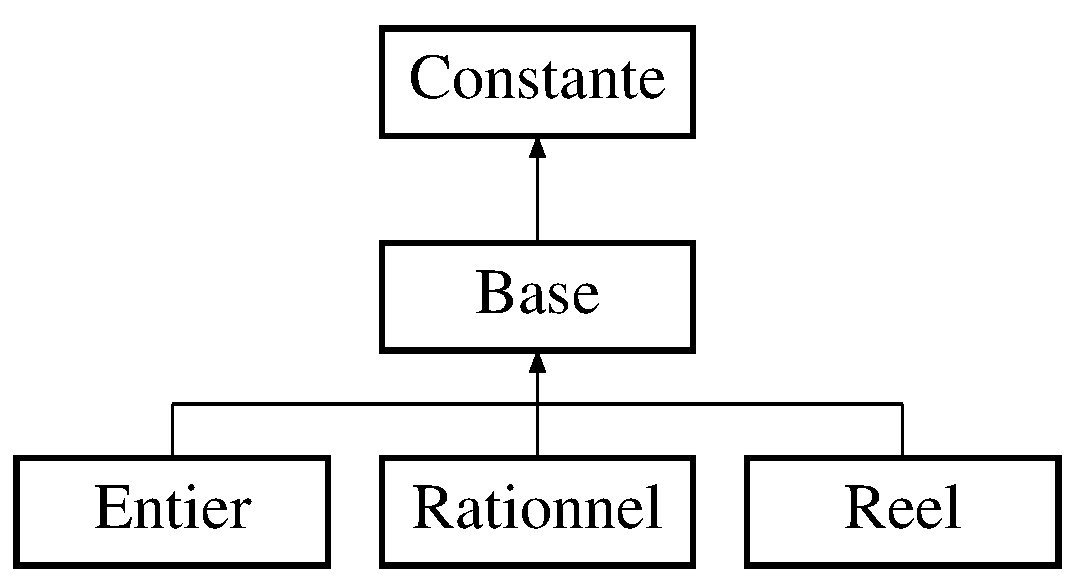
\includegraphics[height=3.000000cm]{class_base}
\end{center}
\end{figure}
\subsection*{Public Member Functions}
\begin{DoxyCompactItemize}
\item 
virtual void \hyperlink{class_base_abf809e43ca06c05dcbe3592648a72466}{Afficher} (std\-::ostream \&os=std\-::cout) const =0
\begin{DoxyCompactList}\small\item\em Fonction virtuelle pour l'affichage. \end{DoxyCompactList}\end{DoxyCompactItemize}


\subsection{Member Function Documentation}
\hypertarget{class_base_abf809e43ca06c05dcbe3592648a72466}{\index{Base@{Base}!Afficher@{Afficher}}
\index{Afficher@{Afficher}!Base@{Base}}
\subsubsection[{Afficher}]{\setlength{\rightskip}{0pt plus 5cm}virtual void Base\-::\-Afficher (
\begin{DoxyParamCaption}
\item[{std\-::ostream \&}]{os = {\ttfamily std\-:\-:cout}}
\end{DoxyParamCaption}
) const\hspace{0.3cm}{\ttfamily [pure virtual]}}}\label{class_base_abf809e43ca06c05dcbe3592648a72466}


Fonction virtuelle pour l'affichage. 


\begin{DoxyParams}{Parameters}
{\em os} & flux d'affichage \\
\hline
\end{DoxyParams}


Implements \hyperlink{class_constante_af3be055efee6c5be81ed6a610dbe2082}{Constante}.



Implemented in \hyperlink{class_entier_ab93c84ba0e96feeaf5cbf8bc4fc7c9c3}{Entier}, \hyperlink{class_rationnel_a52b4a6398d50e630ad76be8be0185f9f}{Rationnel}, and \hyperlink{class_reel_a52eb23de069729bc2f8b8b2c18e1be7d}{Reel}.



The documentation for this class was generated from the following file\-:\begin{DoxyCompactItemize}
\item 
constante.\-h\end{DoxyCompactItemize}

\hypertarget{class_complexe}{\section{Complexe Class Reference}
\label{class_complexe}\index{Complexe@{Complexe}}
}
Inheritance diagram for Complexe\-:\begin{figure}[H]
\begin{center}
\leavevmode
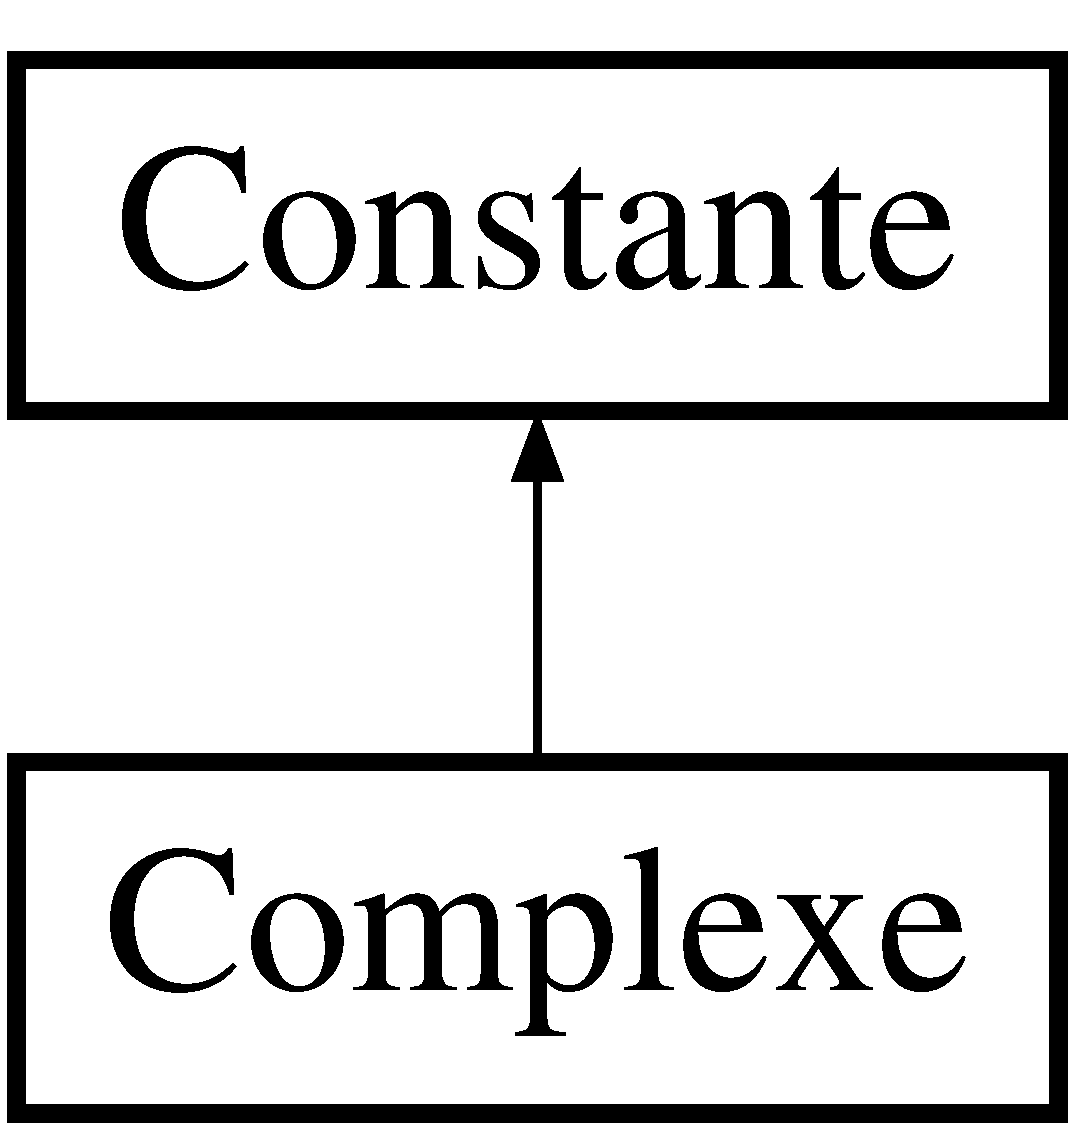
\includegraphics[height=2.000000cm]{class_complexe}
\end{center}
\end{figure}
\subsection*{Public Member Functions}
\begin{DoxyCompactItemize}
\item 
\hypertarget{class_complexe_afbc9334c87c0d03105c6b83cffa91ba6}{{\bfseries Complexe} (\hyperlink{class_base}{Base} $\ast$r, \hyperlink{class_base}{Base} $\ast$i)}\label{class_complexe_afbc9334c87c0d03105c6b83cffa91ba6}

\item 
void \hyperlink{class_complexe_ab81a9988e1a69cae64682e5030de5901}{Afficher} (std\-::ostream \&os=std\-::cout) const 
\begin{DoxyCompactList}\small\item\em Fonction virtuelle pour l'affichage. \end{DoxyCompactList}\item 
double \hyperlink{class_complexe_ab3a3d0582d701ba9fa7ce45d7e82eb81}{Get\-Val} () const 
\item 
double \hyperlink{class_complexe_acfe2a56e2024db9eca2039fccdb2d6f4}{Get\-Val\-Bis} () const 
\item 
\hypertarget{class_complexe_aee55b37e0370e38f3aeedbbf25977876}{const std\-::string {\bfseries Get\-Type} () const }\label{class_complexe_aee55b37e0370e38f3aeedbbf25977876}

\item 
\hypertarget{class_complexe_a32c9167b86fd9cfccb1295c2eecc516e}{Q\-String {\bfseries Get\-Q\-String} () const }\label{class_complexe_a32c9167b86fd9cfccb1295c2eecc516e}

\item 
\hypertarget{class_complexe_a5f39994e59be2809629c9d9deac7539c}{\hyperlink{class_base}{Base} $\ast$ {\bfseries Get\-Reel} () const }\label{class_complexe_a5f39994e59be2809629c9d9deac7539c}

\item 
\hypertarget{class_complexe_ae57b14f197af61edf80f5c0b46373a2f}{\hyperlink{class_base}{Base} $\ast$ {\bfseries Get\-Im} () const }\label{class_complexe_ae57b14f197af61edf80f5c0b46373a2f}

\item 
\hypertarget{class_complexe_a8f564d48149e48b0a0bbb230a6010782}{\hyperlink{class_complexe}{Complexe} \& {\bfseries operator+} (const \hyperlink{class_entier}{Entier} \&)}\label{class_complexe_a8f564d48149e48b0a0bbb230a6010782}

\item 
\hypertarget{class_complexe_a1a2eae6f18f1bd6889ea6d588db49b1f}{\hyperlink{class_complexe}{Complexe} \& {\bfseries operator+} (const \hyperlink{class_reel}{Reel} \&)}\label{class_complexe_a1a2eae6f18f1bd6889ea6d588db49b1f}

\item 
\hypertarget{class_complexe_a0a7497697ce897e1085263b06ea5b0cc}{\hyperlink{class_complexe}{Complexe} \& {\bfseries operator+} (const \hyperlink{class_rationnel}{Rationnel} \&)}\label{class_complexe_a0a7497697ce897e1085263b06ea5b0cc}

\item 
\hypertarget{class_complexe_ac868828ed2144d2ab4b4d3e924877a4d}{\hyperlink{class_complexe}{Complexe} \& {\bfseries operator+} (const \hyperlink{class_complexe}{Complexe} \&)}\label{class_complexe_ac868828ed2144d2ab4b4d3e924877a4d}

\item 
\hypertarget{class_complexe_a251362969154abd42403eea9d9a990dc}{\hyperlink{class_expression}{Expression} \& {\bfseries operator+} (\hyperlink{class_expression}{Expression} \&)}\label{class_complexe_a251362969154abd42403eea9d9a990dc}

\item 
\hypertarget{class_complexe_a2c1cb377233abdbc14bf090eaf0b1fc6}{\hyperlink{class_complexe}{Complexe} \& {\bfseries operator-\/} (const \hyperlink{class_entier}{Entier} \&)}\label{class_complexe_a2c1cb377233abdbc14bf090eaf0b1fc6}

\item 
\hypertarget{class_complexe_aabc15494407881b761d18f4d2669003f}{\hyperlink{class_complexe}{Complexe} \& {\bfseries operator-\/} (const \hyperlink{class_reel}{Reel} \&)}\label{class_complexe_aabc15494407881b761d18f4d2669003f}

\item 
\hypertarget{class_complexe_aecd390424d0b9a59b295fefa1fd651f0}{\hyperlink{class_complexe}{Complexe} \& {\bfseries operator-\/} (const \hyperlink{class_rationnel}{Rationnel} \&)}\label{class_complexe_aecd390424d0b9a59b295fefa1fd651f0}

\item 
\hypertarget{class_complexe_ad940a82652543864ec631747faee8a79}{\hyperlink{class_complexe}{Complexe} \& {\bfseries operator-\/} (const \hyperlink{class_complexe}{Complexe} \&)}\label{class_complexe_ad940a82652543864ec631747faee8a79}

\item 
\hypertarget{class_complexe_a43d1f494d904262cb8a0a3f9c853f722}{\hyperlink{class_expression}{Expression} \& {\bfseries operator-\/} (\hyperlink{class_expression}{Expression} \&)}\label{class_complexe_a43d1f494d904262cb8a0a3f9c853f722}

\item 
\hypertarget{class_complexe_a5355bff31de7a1186c499bcd1fda4471}{\hyperlink{class_complexe}{Complexe} \& {\bfseries operator$\ast$} (const \hyperlink{class_entier}{Entier} \&)}\label{class_complexe_a5355bff31de7a1186c499bcd1fda4471}

\item 
\hypertarget{class_complexe_a94c37dd06b3ab69738ee85606d659597}{\hyperlink{class_complexe}{Complexe} \& {\bfseries operator$\ast$} (const \hyperlink{class_reel}{Reel} \&)}\label{class_complexe_a94c37dd06b3ab69738ee85606d659597}

\item 
\hypertarget{class_complexe_ac4ea1c9d3dacef53efd12fe97d07163f}{\hyperlink{class_complexe}{Complexe} \& {\bfseries operator$\ast$} (const \hyperlink{class_rationnel}{Rationnel} \&)}\label{class_complexe_ac4ea1c9d3dacef53efd12fe97d07163f}

\item 
\hypertarget{class_complexe_a3814fe630d3b141212721dacc1d5bcda}{\hyperlink{class_complexe}{Complexe} \& {\bfseries operator$\ast$} (const \hyperlink{class_complexe}{Complexe} \&)}\label{class_complexe_a3814fe630d3b141212721dacc1d5bcda}

\item 
\hypertarget{class_complexe_a0e8ca6bde04a305add0ea3a047010d6e}{\hyperlink{class_expression}{Expression} \& {\bfseries operator$\ast$} (\hyperlink{class_expression}{Expression} \&)}\label{class_complexe_a0e8ca6bde04a305add0ea3a047010d6e}

\item 
\hypertarget{class_complexe_a32ed305645e63f7b2151c8dc7c7df76f}{\hyperlink{class_complexe}{Complexe} \& {\bfseries operator/} (const \hyperlink{class_entier}{Entier} \&)}\label{class_complexe_a32ed305645e63f7b2151c8dc7c7df76f}

\item 
\hypertarget{class_complexe_aed3d758e4a4e56660511d0fb41a82786}{\hyperlink{class_complexe}{Complexe} \& {\bfseries operator/} (const \hyperlink{class_reel}{Reel} \&)}\label{class_complexe_aed3d758e4a4e56660511d0fb41a82786}

\item 
\hypertarget{class_complexe_a52013dde54f2fd70750421ebf862aef4}{\hyperlink{class_complexe}{Complexe} \& {\bfseries operator/} (const \hyperlink{class_rationnel}{Rationnel} \&)}\label{class_complexe_a52013dde54f2fd70750421ebf862aef4}

\item 
\hypertarget{class_complexe_a23e5c1600cb8c0a63fbd6e8b67bd9dc1}{\hyperlink{class_complexe}{Complexe} \& {\bfseries operator/} (const \hyperlink{class_complexe}{Complexe} \&)}\label{class_complexe_a23e5c1600cb8c0a63fbd6e8b67bd9dc1}

\item 
\hypertarget{class_complexe_ab09b368175de16af6caa91b1f898882d}{\hyperlink{class_expression}{Expression} \& {\bfseries operator/} (\hyperlink{class_expression}{Expression} \&)}\label{class_complexe_ab09b368175de16af6caa91b1f898882d}

\item 
\hypertarget{class_complexe_afda6d543bb4195b86b367213659ffb91}{\hyperlink{class_complexe}{Complexe} \& {\bfseries cos\-Fonction} (std\-::string)}\label{class_complexe_afda6d543bb4195b86b367213659ffb91}

\item 
\hypertarget{class_complexe_a99fa7640f8e49a8cff859f74480b9ce6}{\hyperlink{class_complexe}{Complexe} \& {\bfseries sin\-Fonction} (std\-::string)}\label{class_complexe_a99fa7640f8e49a8cff859f74480b9ce6}

\item 
\hypertarget{class_complexe_aaaefd1999856bb13c6df425cc7c6f34c}{\hyperlink{class_complexe}{Complexe} \& {\bfseries tan\-Fonction} (std\-::string)}\label{class_complexe_aaaefd1999856bb13c6df425cc7c6f34c}

\item 
\hypertarget{class_complexe_a1bdd47084fa06f2275d553d85d76c1e0}{\hyperlink{class_complexe}{Complexe} \& {\bfseries cosh\-Fonction} (std\-::string)}\label{class_complexe_a1bdd47084fa06f2275d553d85d76c1e0}

\item 
\hypertarget{class_complexe_a7568b17feb57979a9e4e7124add5b748}{\hyperlink{class_complexe}{Complexe} \& {\bfseries sinh\-Fonction} (std\-::string)}\label{class_complexe_a7568b17feb57979a9e4e7124add5b748}

\item 
\hypertarget{class_complexe_a36fdf178593fc28651c4b19c5abfa03a}{\hyperlink{class_complexe}{Complexe} \& {\bfseries tanh\-Fonction} (std\-::string)}\label{class_complexe_a36fdf178593fc28651c4b19c5abfa03a}

\item 
\hypertarget{class_complexe_a88399a019d3a1acd7ecd2bbfa7b19674}{\hyperlink{class_complexe}{Complexe} \& {\bfseries pow\-Fonction} (const \hyperlink{class_entier}{Entier} \&)}\label{class_complexe_a88399a019d3a1acd7ecd2bbfa7b19674}

\item 
\hypertarget{class_complexe_a083ffc2f19c4a8b2ca45cb574337d39b}{\hyperlink{class_complexe}{Complexe} \& {\bfseries pow\-Fonction} (const \hyperlink{class_reel}{Reel} \&)}\label{class_complexe_a083ffc2f19c4a8b2ca45cb574337d39b}

\item 
\hypertarget{class_complexe_a45212d194eed3e1984a215aa319c76d6}{\hyperlink{class_complexe}{Complexe} \& {\bfseries pow\-Fonction} (const \hyperlink{class_rationnel}{Rationnel} \&)}\label{class_complexe_a45212d194eed3e1984a215aa319c76d6}

\item 
\hypertarget{class_complexe_aaa0a23fd4ef264b8929a378b4a529c57}{\hyperlink{class_complexe}{Complexe} \& {\bfseries pow\-Fonction} (\hyperlink{class_expression}{Expression} \&)}\label{class_complexe_aaa0a23fd4ef264b8929a378b4a529c57}

\item 
\hypertarget{class_complexe_a0aa584da80d7291bec0984db5c37f097}{\hyperlink{class_complexe}{Complexe} \& {\bfseries pow\-Fonction} (const \hyperlink{class_complexe}{Complexe} \&)}\label{class_complexe_a0aa584da80d7291bec0984db5c37f097}

\end{DoxyCompactItemize}


\subsection{Member Function Documentation}
\hypertarget{class_complexe_ab81a9988e1a69cae64682e5030de5901}{\index{Complexe@{Complexe}!Afficher@{Afficher}}
\index{Afficher@{Afficher}!Complexe@{Complexe}}
\subsubsection[{Afficher}]{\setlength{\rightskip}{0pt plus 5cm}void Complexe\-::\-Afficher (
\begin{DoxyParamCaption}
\item[{std\-::ostream \&}]{os = {\ttfamily std\-:\-:cout}}
\end{DoxyParamCaption}
) const\hspace{0.3cm}{\ttfamily [inline]}, {\ttfamily [virtual]}}}\label{class_complexe_ab81a9988e1a69cae64682e5030de5901}


Fonction virtuelle pour l'affichage. 


\begin{DoxyParams}{Parameters}
{\em os} & flux d'affichage \\
\hline
\end{DoxyParams}


Implements \hyperlink{class_constante_af3be055efee6c5be81ed6a610dbe2082}{Constante}.

\hypertarget{class_complexe_ab3a3d0582d701ba9fa7ce45d7e82eb81}{\index{Complexe@{Complexe}!Get\-Val@{Get\-Val}}
\index{Get\-Val@{Get\-Val}!Complexe@{Complexe}}
\subsubsection[{Get\-Val}]{\setlength{\rightskip}{0pt plus 5cm}double Complexe\-::\-Get\-Val (
\begin{DoxyParamCaption}
{}
\end{DoxyParamCaption}
) const\hspace{0.3cm}{\ttfamily [inline]}, {\ttfamily [virtual]}}}\label{class_complexe_ab3a3d0582d701ba9fa7ce45d7e82eb81}
\begin{DoxyReturn}{Returns}
Renvoie un double qui représente une valeur principale de la classe. 
\end{DoxyReturn}


Implements \hyperlink{class_constante_af88eb444ed659cc6bb2f9571326a9eb1}{Constante}.

\hypertarget{class_complexe_acfe2a56e2024db9eca2039fccdb2d6f4}{\index{Complexe@{Complexe}!Get\-Val\-Bis@{Get\-Val\-Bis}}
\index{Get\-Val\-Bis@{Get\-Val\-Bis}!Complexe@{Complexe}}
\subsubsection[{Get\-Val\-Bis}]{\setlength{\rightskip}{0pt plus 5cm}double Complexe\-::\-Get\-Val\-Bis (
\begin{DoxyParamCaption}
{}
\end{DoxyParamCaption}
) const\hspace{0.3cm}{\ttfamily [inline]}, {\ttfamily [virtual]}}}\label{class_complexe_acfe2a56e2024db9eca2039fccdb2d6f4}
\begin{DoxyReturn}{Returns}
Renvoie un double qui représente une valeur secondaire de la classe. 
\end{DoxyReturn}


Implements \hyperlink{class_constante_aa0602d62c04f28f7bda68723f5dbc48b}{Constante}.



The documentation for this class was generated from the following files\-:\begin{DoxyCompactItemize}
\item 
constante.\-h\item 
constante\-Op\-Div.\-cpp\item 
constante\-Op\-Moins.\-cpp\item 
constante\-Op\-Mult.\-cpp\item 
constante\-Op\-Plus.\-cpp\item 
constante\-Op\-Pow.\-cpp\item 
operateurs\-Unaires.\-cpp\end{DoxyCompactItemize}

\hypertarget{class_constante}{\section{Constante Class Reference}
\label{class_constante}\index{Constante@{Constante}}
}


Classe mère de toutes les valeurs empilées dans la pile de stockage.  




{\ttfamily \#include $<$constante.\-h$>$}

Inheritance diagram for Constante\-:\begin{figure}[H]
\begin{center}
\leavevmode
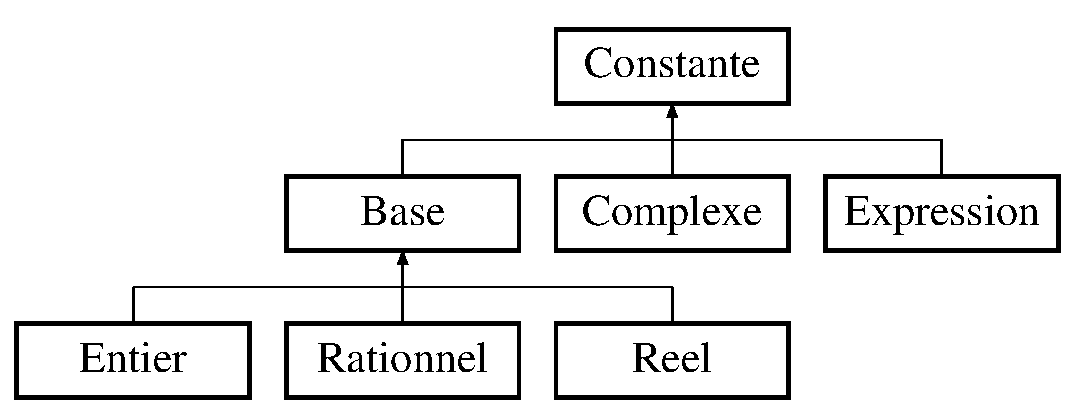
\includegraphics[height=3.000000cm]{class_constante}
\end{center}
\end{figure}
\subsection*{Public Member Functions}
\begin{DoxyCompactItemize}
\item 
virtual void \hyperlink{class_constante_af3be055efee6c5be81ed6a610dbe2082}{Afficher} (std\-::ostream \&os=std\-::cout) const =0
\begin{DoxyCompactList}\small\item\em Fonction virtuelle pour l'affichage. \end{DoxyCompactList}\item 
virtual double \hyperlink{class_constante_af88eb444ed659cc6bb2f9571326a9eb1}{Get\-Val} () const =0
\item 
virtual double \hyperlink{class_constante_aa0602d62c04f28f7bda68723f5dbc48b}{Get\-Val\-Bis} () const =0
\item 
\hypertarget{class_constante_a2f716a85b9b519b7bbf8ed8d997f66d3}{virtual const std\-::string {\bfseries Get\-Type} () const =0}\label{class_constante_a2f716a85b9b519b7bbf8ed8d997f66d3}

\item 
\hypertarget{class_constante_a7c3edb9082492c95eb319da3d42bb7a4}{virtual Q\-String {\bfseries Get\-Q\-String} () const =0}\label{class_constante_a7c3edb9082492c95eb319da3d42bb7a4}

\item 
\hypertarget{class_constante_a19f83499c795b8fc069eb18600d4150b}{virtual void {\bfseries Simplifier} ()}\label{class_constante_a19f83499c795b8fc069eb18600d4150b}

\item 
\hypertarget{class_constante_a2346d7608b9732c34f96d01bed7de6c1}{virtual \hyperlink{class_constante}{Constante} \& {\bfseries operator+} (\hyperlink{class_constante}{Constante} $\ast$)}\label{class_constante_a2346d7608b9732c34f96d01bed7de6c1}

\item 
\hypertarget{class_constante_adb952a391e582f997a96d848e461e281}{virtual \hyperlink{class_constante}{Constante} \& {\bfseries operator+} (const \hyperlink{class_reel}{Reel} \&)=0}\label{class_constante_adb952a391e582f997a96d848e461e281}

\item 
\hypertarget{class_constante_a2402e4cd1b0d9d9618f05fe5876f090f}{virtual \hyperlink{class_constante}{Constante} \& {\bfseries operator+} (const \hyperlink{class_entier}{Entier} \&)=0}\label{class_constante_a2402e4cd1b0d9d9618f05fe5876f090f}

\item 
\hypertarget{class_constante_ad778cc57ca2edc0bc09dc63455029451}{virtual \hyperlink{class_constante}{Constante} \& {\bfseries operator+} (const \hyperlink{class_rationnel}{Rationnel} \&)=0}\label{class_constante_ad778cc57ca2edc0bc09dc63455029451}

\item 
\hypertarget{class_constante_a753901cb5653de58594c74038536f56b}{virtual \hyperlink{class_constante}{Constante} \& {\bfseries operator+} (const \hyperlink{class_complexe}{Complexe} \&)=0}\label{class_constante_a753901cb5653de58594c74038536f56b}

\item 
\hypertarget{class_constante_a03fc01b8fdf5b8945ae8b72209bc1285}{virtual \hyperlink{class_constante}{Constante} \& {\bfseries operator+} (\hyperlink{class_expression}{Expression} \&)=0}\label{class_constante_a03fc01b8fdf5b8945ae8b72209bc1285}

\item 
\hypertarget{class_constante_a24a763c775e35399bff4441b2f41db12}{virtual \hyperlink{class_constante}{Constante} \& {\bfseries operator-\/} (\hyperlink{class_constante}{Constante} $\ast$)}\label{class_constante_a24a763c775e35399bff4441b2f41db12}

\item 
\hypertarget{class_constante_a6eb6194c90dce85b0e8d55cb39733f6e}{virtual \hyperlink{class_constante}{Constante} \& {\bfseries operator-\/} (const \hyperlink{class_reel}{Reel} \&)=0}\label{class_constante_a6eb6194c90dce85b0e8d55cb39733f6e}

\item 
\hypertarget{class_constante_a0227e180269d318299bf7981a639d196}{virtual \hyperlink{class_constante}{Constante} \& {\bfseries operator-\/} (const \hyperlink{class_entier}{Entier} \&)=0}\label{class_constante_a0227e180269d318299bf7981a639d196}

\item 
\hypertarget{class_constante_aa525b610edbed58856836181b8ea78f8}{virtual \hyperlink{class_constante}{Constante} \& {\bfseries operator-\/} (const \hyperlink{class_rationnel}{Rationnel} \&)=0}\label{class_constante_aa525b610edbed58856836181b8ea78f8}

\item 
\hypertarget{class_constante_aa8f176be374c96fbe1c24716eabf9b07}{virtual \hyperlink{class_constante}{Constante} \& {\bfseries operator-\/} (const \hyperlink{class_complexe}{Complexe} \&)=0}\label{class_constante_aa8f176be374c96fbe1c24716eabf9b07}

\item 
\hypertarget{class_constante_aca98518ee0933a3eabe01da0739e36be}{virtual \hyperlink{class_constante}{Constante} \& {\bfseries operator-\/} (\hyperlink{class_expression}{Expression} \&)=0}\label{class_constante_aca98518ee0933a3eabe01da0739e36be}

\item 
\hypertarget{class_constante_a4293c8632cc246b0e88285ae4afd2128}{virtual \hyperlink{class_constante}{Constante} \& {\bfseries operator$\ast$} (\hyperlink{class_constante}{Constante} $\ast$)}\label{class_constante_a4293c8632cc246b0e88285ae4afd2128}

\item 
\hypertarget{class_constante_a44b5993c7da0b9e89a40980f2bcb8f1e}{virtual \hyperlink{class_constante}{Constante} \& {\bfseries operator$\ast$} (const \hyperlink{class_reel}{Reel} \&)=0}\label{class_constante_a44b5993c7da0b9e89a40980f2bcb8f1e}

\item 
\hypertarget{class_constante_aeabf86524c5dca456de99068eff0faa0}{virtual \hyperlink{class_constante}{Constante} \& {\bfseries operator$\ast$} (const \hyperlink{class_entier}{Entier} \&)=0}\label{class_constante_aeabf86524c5dca456de99068eff0faa0}

\item 
\hypertarget{class_constante_a4b7d7328c364c30e53c5045eea6fe58c}{virtual \hyperlink{class_constante}{Constante} \& {\bfseries operator$\ast$} (const \hyperlink{class_rationnel}{Rationnel} \&)=0}\label{class_constante_a4b7d7328c364c30e53c5045eea6fe58c}

\item 
\hypertarget{class_constante_a65a3360420827c4c7953052ff87b2457}{virtual \hyperlink{class_constante}{Constante} \& {\bfseries operator$\ast$} (const \hyperlink{class_complexe}{Complexe} \&)=0}\label{class_constante_a65a3360420827c4c7953052ff87b2457}

\item 
\hypertarget{class_constante_a51016ec3398e1a5f2ba4cea752c5c7db}{virtual \hyperlink{class_constante}{Constante} \& {\bfseries operator$\ast$} (\hyperlink{class_expression}{Expression} \&)=0}\label{class_constante_a51016ec3398e1a5f2ba4cea752c5c7db}

\item 
\hypertarget{class_constante_a9be1827fd118f5a81cf10b509b64cfa7}{virtual \hyperlink{class_constante}{Constante} \& {\bfseries operator/} (\hyperlink{class_constante}{Constante} $\ast$)}\label{class_constante_a9be1827fd118f5a81cf10b509b64cfa7}

\item 
\hypertarget{class_constante_a0355225f82499fabe7e64a5a09866fdb}{virtual \hyperlink{class_constante}{Constante} \& {\bfseries operator/} (const \hyperlink{class_reel}{Reel} \&)=0}\label{class_constante_a0355225f82499fabe7e64a5a09866fdb}

\item 
\hypertarget{class_constante_ac90f8c29c86fa9ccb15a44c64b14ee87}{virtual \hyperlink{class_constante}{Constante} \& {\bfseries operator/} (const \hyperlink{class_entier}{Entier} \&)=0}\label{class_constante_ac90f8c29c86fa9ccb15a44c64b14ee87}

\item 
\hypertarget{class_constante_a8c0dfdc199f6a8feff5038abf75c2b98}{virtual \hyperlink{class_constante}{Constante} \& {\bfseries operator/} (const \hyperlink{class_rationnel}{Rationnel} \&)=0}\label{class_constante_a8c0dfdc199f6a8feff5038abf75c2b98}

\item 
\hypertarget{class_constante_a5944c154c12015c0af36ef5fdb2e851b}{virtual \hyperlink{class_constante}{Constante} \& {\bfseries operator/} (const \hyperlink{class_complexe}{Complexe} \&)=0}\label{class_constante_a5944c154c12015c0af36ef5fdb2e851b}

\item 
\hypertarget{class_constante_a2c2e07511d0e5883ef337351b2121606}{virtual \hyperlink{class_constante}{Constante} \& {\bfseries operator/} (\hyperlink{class_expression}{Expression} \&)=0}\label{class_constante_a2c2e07511d0e5883ef337351b2121606}

\item 
\hypertarget{class_constante_a9234f524cc1b97560236afe686c4767a}{virtual \hyperlink{class_constante}{Constante} \& {\bfseries operator\%} (\hyperlink{class_constante}{Constante} $\ast$)}\label{class_constante_a9234f524cc1b97560236afe686c4767a}

\item 
\hypertarget{class_constante_a62ac7c7b4f04706ef930728736ee45ae}{virtual \hyperlink{class_constante}{Constante} \& {\bfseries cos\-Fonction} (std\-::string)=0}\label{class_constante_a62ac7c7b4f04706ef930728736ee45ae}

\item 
\hypertarget{class_constante_adf047fc87a4bc192ca159ad1711effb2}{virtual \hyperlink{class_constante}{Constante} \& {\bfseries sin\-Fonction} (std\-::string)=0}\label{class_constante_adf047fc87a4bc192ca159ad1711effb2}

\item 
\hypertarget{class_constante_ac527584889c9865e0dc80e4c22f6fc73}{virtual \hyperlink{class_constante}{Constante} \& {\bfseries tan\-Fonction} (std\-::string)=0}\label{class_constante_ac527584889c9865e0dc80e4c22f6fc73}

\item 
\hypertarget{class_constante_ae0bf50b47928dc108de2f29231aefbeb}{virtual \hyperlink{class_constante}{Constante} \& {\bfseries cosh\-Fonction} (std\-::string)=0}\label{class_constante_ae0bf50b47928dc108de2f29231aefbeb}

\item 
\hypertarget{class_constante_adbdbe6e979fcdf68d2c38c8114d0dde6}{virtual \hyperlink{class_constante}{Constante} \& {\bfseries sinh\-Fonction} (std\-::string)=0}\label{class_constante_adbdbe6e979fcdf68d2c38c8114d0dde6}

\item 
\hypertarget{class_constante_a79f9e32d8dfe2980f9ad17733d5905fb}{virtual \hyperlink{class_constante}{Constante} \& {\bfseries tanh\-Fonction} (std\-::string)=0}\label{class_constante_a79f9e32d8dfe2980f9ad17733d5905fb}

\item 
\hypertarget{class_constante_a6218e67aef6b06f29d37b112206d56c6}{virtual \hyperlink{class_constante}{Constante} \& {\bfseries pow\-Fonction} (\hyperlink{class_constante}{Constante} $\ast$)}\label{class_constante_a6218e67aef6b06f29d37b112206d56c6}

\item 
\hypertarget{class_constante_a4de24bbfec26b381782d54f86699f5db}{virtual \hyperlink{class_constante}{Constante} \& {\bfseries pow\-Fonction} (const \hyperlink{class_entier}{Entier} \&)=0}\label{class_constante_a4de24bbfec26b381782d54f86699f5db}

\item 
\hypertarget{class_constante_aac4655c82f3adc298c242c1858a185de}{virtual \hyperlink{class_constante}{Constante} \& {\bfseries pow\-Fonction} (const \hyperlink{class_reel}{Reel} \&)=0}\label{class_constante_aac4655c82f3adc298c242c1858a185de}

\item 
\hypertarget{class_constante_acfa643e1f95d98b3eafb4275bbb533d5}{virtual \hyperlink{class_constante}{Constante} \& {\bfseries pow\-Fonction} (const \hyperlink{class_rationnel}{Rationnel} \&)=0}\label{class_constante_acfa643e1f95d98b3eafb4275bbb533d5}

\item 
\hypertarget{class_constante_aae63d1d974ef6fe0f516ce1cfcaff5eb}{virtual \hyperlink{class_constante}{Constante} \& {\bfseries pow\-Fonction} (const \hyperlink{class_complexe}{Complexe} \&)=0}\label{class_constante_aae63d1d974ef6fe0f516ce1cfcaff5eb}

\item 
\hypertarget{class_constante_ae7639614d627f4a87e477095e65b4896}{virtual \hyperlink{class_constante}{Constante} \& {\bfseries pow\-Fonction} (\hyperlink{class_expression}{Expression} \&)=0}\label{class_constante_ae7639614d627f4a87e477095e65b4896}

\item 
\hypertarget{class_constante_a52dd5fcfeb66534183e9419c222c6960}{virtual \hyperlink{class_constante}{Constante} \& {\bfseries fact\-Fonction} ()}\label{class_constante_a52dd5fcfeb66534183e9419c222c6960}

\item 
\hypertarget{class_constante_abf6fa0c8026ebcbf5c1a0d55b56f5d5b}{virtual \hyperlink{class_constante}{Constante} \& {\bfseries sign\-Fonction} ()}\label{class_constante_abf6fa0c8026ebcbf5c1a0d55b56f5d5b}

\item 
\hypertarget{class_constante_a89475969e57f022a38cc3fb6617e3e29}{virtual \hyperlink{class_constante}{Constante} \& {\bfseries sqr\-Fonction} ()}\label{class_constante_a89475969e57f022a38cc3fb6617e3e29}

\item 
\hypertarget{class_constante_a19851e590e8c40a4f3fddd3e78780a05}{virtual \hyperlink{class_constante}{Constante} \& {\bfseries cube\-Fonction} ()}\label{class_constante_a19851e590e8c40a4f3fddd3e78780a05}

\item 
\hypertarget{class_constante_a94668c82b50be66607e701d989d5f725}{virtual \hyperlink{class_constante}{Constante} \& {\bfseries sqrt\-Fonction} ()}\label{class_constante_a94668c82b50be66607e701d989d5f725}

\item 
\hypertarget{class_constante_aa6b78608f1cac4f73fd6fc329827fc51}{virtual \hyperlink{class_constante}{Constante} \& {\bfseries inv\-Fonction} ()}\label{class_constante_aa6b78608f1cac4f73fd6fc329827fc51}

\end{DoxyCompactItemize}


\subsection{Detailed Description}
Classe mère de toutes les valeurs empilées dans la pile de stockage. 

\subsection{Member Function Documentation}
\hypertarget{class_constante_af3be055efee6c5be81ed6a610dbe2082}{\index{Constante@{Constante}!Afficher@{Afficher}}
\index{Afficher@{Afficher}!Constante@{Constante}}
\subsubsection[{Afficher}]{\setlength{\rightskip}{0pt plus 5cm}virtual void Constante\-::\-Afficher (
\begin{DoxyParamCaption}
\item[{std\-::ostream \&}]{os = {\ttfamily std\-:\-:cout}}
\end{DoxyParamCaption}
) const\hspace{0.3cm}{\ttfamily [pure virtual]}}}\label{class_constante_af3be055efee6c5be81ed6a610dbe2082}


Fonction virtuelle pour l'affichage. 


\begin{DoxyParams}{Parameters}
{\em os} & flux d'affichage \\
\hline
\end{DoxyParams}


Implemented in \hyperlink{class_entier_ab93c84ba0e96feeaf5cbf8bc4fc7c9c3}{Entier}, \hyperlink{class_rationnel_a52b4a6398d50e630ad76be8be0185f9f}{Rationnel}, \hyperlink{class_reel_a52eb23de069729bc2f8b8b2c18e1be7d}{Reel}, \hyperlink{class_complexe_ab81a9988e1a69cae64682e5030de5901}{Complexe}, \hyperlink{class_base_abf809e43ca06c05dcbe3592648a72466}{Base}, and \hyperlink{class_expression_a82c745bad73c0adf286f893febaf7406}{Expression}.

\hypertarget{class_constante_af88eb444ed659cc6bb2f9571326a9eb1}{\index{Constante@{Constante}!Get\-Val@{Get\-Val}}
\index{Get\-Val@{Get\-Val}!Constante@{Constante}}
\subsubsection[{Get\-Val}]{\setlength{\rightskip}{0pt plus 5cm}virtual double Constante\-::\-Get\-Val (
\begin{DoxyParamCaption}
{}
\end{DoxyParamCaption}
) const\hspace{0.3cm}{\ttfamily [pure virtual]}}}\label{class_constante_af88eb444ed659cc6bb2f9571326a9eb1}
\begin{DoxyReturn}{Returns}
Renvoie un double qui représente une valeur principale de la classe. 
\end{DoxyReturn}


Implemented in \hyperlink{class_entier_a3e5f576f451df416bb58e7286ccbe951}{Entier}, \hyperlink{class_rationnel_a29987744cb2a7631ffa4db708630fe19}{Rationnel}, \hyperlink{class_reel_a5755a5ed2d9042ad59984967dbddc7f5}{Reel}, \hyperlink{class_complexe_ab3a3d0582d701ba9fa7ce45d7e82eb81}{Complexe}, and \hyperlink{class_expression_addc8118b94c445af0da80e8e661dfd6a}{Expression}.

\hypertarget{class_constante_aa0602d62c04f28f7bda68723f5dbc48b}{\index{Constante@{Constante}!Get\-Val\-Bis@{Get\-Val\-Bis}}
\index{Get\-Val\-Bis@{Get\-Val\-Bis}!Constante@{Constante}}
\subsubsection[{Get\-Val\-Bis}]{\setlength{\rightskip}{0pt plus 5cm}virtual double Constante\-::\-Get\-Val\-Bis (
\begin{DoxyParamCaption}
{}
\end{DoxyParamCaption}
) const\hspace{0.3cm}{\ttfamily [pure virtual]}}}\label{class_constante_aa0602d62c04f28f7bda68723f5dbc48b}
\begin{DoxyReturn}{Returns}
Renvoie un double qui représente une valeur secondaire de la classe. 
\end{DoxyReturn}


Implemented in \hyperlink{class_entier_a349675638599cd6e5f67161664e1d58a}{Entier}, \hyperlink{class_rationnel_a2403f411e88b3de9f83ad735342e68ec}{Rationnel}, \hyperlink{class_reel_ab66ca2cb446b1cbc0c3565ff054acc1b}{Reel}, \hyperlink{class_complexe_acfe2a56e2024db9eca2039fccdb2d6f4}{Complexe}, and \hyperlink{class_expression_ad602729011040226673d7c1ee94367d9}{Expression}.



The documentation for this class was generated from the following files\-:\begin{DoxyCompactItemize}
\item 
constante.\-h\item 
constante\-Op\-Div.\-cpp\item 
constante\-Op\-Mod.\-cpp\item 
constante\-Op\-Moins.\-cpp\item 
constante\-Op\-Mult.\-cpp\item 
constante\-Op\-Plus.\-cpp\item 
constante\-Op\-Pow.\-cpp\item 
operateurs\-Unaires.\-cpp\end{DoxyCompactItemize}

\hypertarget{class_entier}{\section{Entier Class Reference}
\label{class_entier}\index{Entier@{Entier}}
}


Classe permettant de représenter le type \hyperlink{class_entier}{Entier}.  




{\ttfamily \#include $<$constante.\-h$>$}

Inheritance diagram for Entier\-:\begin{figure}[H]
\begin{center}
\leavevmode
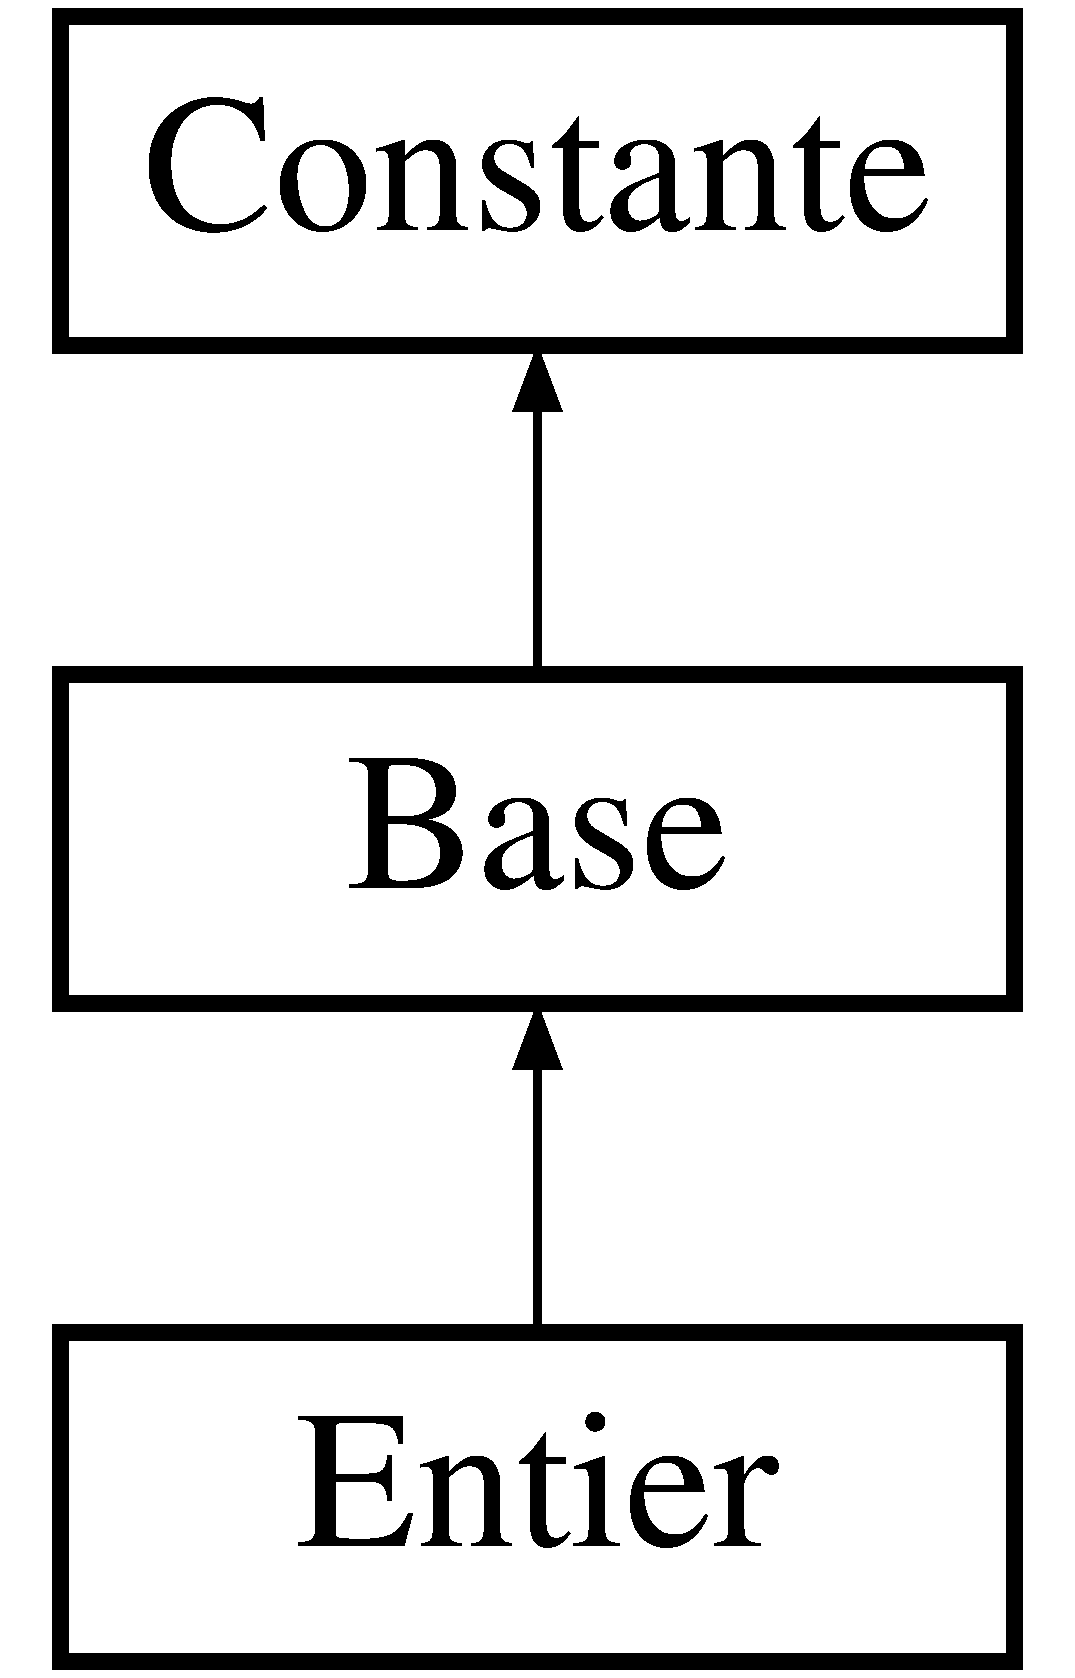
\includegraphics[height=3.000000cm]{class_entier}
\end{center}
\end{figure}
\subsection*{Public Member Functions}
\begin{DoxyCompactItemize}
\item 
\hypertarget{class_entier_a3c5a9dc84dc805fb47be686f35dca765}{{\bfseries Entier} (int n=0)}\label{class_entier_a3c5a9dc84dc805fb47be686f35dca765}

\item 
\hypertarget{class_entier_a6a50b62869bbefdc15286c05faeaa54f}{{\bfseries Entier} (Q\-String s)}\label{class_entier_a6a50b62869bbefdc15286c05faeaa54f}

\item 
void \hyperlink{class_entier_ab93c84ba0e96feeaf5cbf8bc4fc7c9c3}{Afficher} (std\-::ostream \&os=std\-::cout) const 
\begin{DoxyCompactList}\small\item\em Fonction virtuelle pour l'affichage, affichant une constante en console. \end{DoxyCompactList}\item 
double \hyperlink{class_entier_a3e5f576f451df416bb58e7286ccbe951}{Get\-Val} () const 
\begin{DoxyCompactList}\small\item\em Fonction permettant de récupérer la valeur principale des différentes constantes. \end{DoxyCompactList}\item 
double \hyperlink{class_entier_a349675638599cd6e5f67161664e1d58a}{Get\-Val\-Bis} () const 
\begin{DoxyCompactList}\small\item\em Fonction permettant de récupérer la valeur secondaire des différentes constantes. \end{DoxyCompactList}\item 
const std\-::string \hyperlink{class_entier_af8701306da8ca2e12869eaa3c65eb03b}{Get\-Type} () const 
\begin{DoxyCompactList}\small\item\em Fonction permettant de récupérer la valeur du type des différentes constantes. \end{DoxyCompactList}\item 
Q\-String \hyperlink{class_entier_a6e534c8d7e3861fd43055134f4379262}{Get\-Q\-String} () const 
\begin{DoxyCompactList}\small\item\em Fonction permettant de transformer une \hyperlink{class_constante}{Constante} en Q\-String. \end{DoxyCompactList}\item 
\hypertarget{class_entier_aea9f797a407f40195fe41b0c151b4ad9}{\hyperlink{class_entier}{Entier} \& {\bfseries operator+} (const \hyperlink{class_entier}{Entier} \&)}\label{class_entier_aea9f797a407f40195fe41b0c151b4ad9}

\item 
\hypertarget{class_entier_a6e29bfb969436e9c3bc10a728593532d}{\hyperlink{class_reel}{Reel} \& {\bfseries operator+} (const \hyperlink{class_reel}{Reel} \&)}\label{class_entier_a6e29bfb969436e9c3bc10a728593532d}

\item 
\hypertarget{class_entier_a9a8f4bb64e5eccc82cf445098ef7f4b6}{\hyperlink{class_rationnel}{Rationnel} \& {\bfseries operator+} (const \hyperlink{class_rationnel}{Rationnel} \&)}\label{class_entier_a9a8f4bb64e5eccc82cf445098ef7f4b6}

\item 
\hypertarget{class_entier_adc0b1960001fc3037a575c74435fd323}{\hyperlink{class_complexe}{Complexe} \& {\bfseries operator+} (const \hyperlink{class_complexe}{Complexe} \&)}\label{class_entier_adc0b1960001fc3037a575c74435fd323}

\item 
\hypertarget{class_entier_a74cc330ea474e84f522c554de4ec668c}{\hyperlink{class_expression}{Expression} \& {\bfseries operator+} (\hyperlink{class_expression}{Expression} \&)}\label{class_entier_a74cc330ea474e84f522c554de4ec668c}

\item 
\hypertarget{class_entier_ac4921c3144117cb96ce7af0ae7f9259a}{\hyperlink{class_entier}{Entier} \& {\bfseries operator-\/} (const \hyperlink{class_entier}{Entier} \&)}\label{class_entier_ac4921c3144117cb96ce7af0ae7f9259a}

\item 
\hypertarget{class_entier_a7537c188456ee327ab74f55c20c60bf4}{\hyperlink{class_reel}{Reel} \& {\bfseries operator-\/} (const \hyperlink{class_reel}{Reel} \&)}\label{class_entier_a7537c188456ee327ab74f55c20c60bf4}

\item 
\hypertarget{class_entier_a82bec61f84bc9a7b179515a200de28af}{\hyperlink{class_rationnel}{Rationnel} \& {\bfseries operator-\/} (const \hyperlink{class_rationnel}{Rationnel} \&)}\label{class_entier_a82bec61f84bc9a7b179515a200de28af}

\item 
\hypertarget{class_entier_a1c92191694534d5704ac95732179e82e}{\hyperlink{class_complexe}{Complexe} \& {\bfseries operator-\/} (const \hyperlink{class_complexe}{Complexe} \&)}\label{class_entier_a1c92191694534d5704ac95732179e82e}

\item 
\hypertarget{class_entier_aafc4192c799ef36c71a0b86d5105fc11}{\hyperlink{class_expression}{Expression} \& {\bfseries operator-\/} (\hyperlink{class_expression}{Expression} \&)}\label{class_entier_aafc4192c799ef36c71a0b86d5105fc11}

\item 
\hypertarget{class_entier_a409f671c6083fa7eea4e6942d90b1d00}{\hyperlink{class_entier}{Entier} \& {\bfseries operator$\ast$} (const \hyperlink{class_entier}{Entier} \&)}\label{class_entier_a409f671c6083fa7eea4e6942d90b1d00}

\item 
\hypertarget{class_entier_a59f9cc2fbd1ab426c83458a3911c10e9}{\hyperlink{class_reel}{Reel} \& {\bfseries operator$\ast$} (const \hyperlink{class_reel}{Reel} \&)}\label{class_entier_a59f9cc2fbd1ab426c83458a3911c10e9}

\item 
\hypertarget{class_entier_a5699e20cbcee3c10aa01a77b877f60c0}{\hyperlink{class_rationnel}{Rationnel} \& {\bfseries operator$\ast$} (const \hyperlink{class_rationnel}{Rationnel} \&)}\label{class_entier_a5699e20cbcee3c10aa01a77b877f60c0}

\item 
\hypertarget{class_entier_ab07e9f33e533a3f87a3e8dbda76dcaf7}{\hyperlink{class_complexe}{Complexe} \& {\bfseries operator$\ast$} (const \hyperlink{class_complexe}{Complexe} \&)}\label{class_entier_ab07e9f33e533a3f87a3e8dbda76dcaf7}

\item 
\hypertarget{class_entier_a701848b80d49caa017878fb51b9f9506}{\hyperlink{class_expression}{Expression} \& {\bfseries operator$\ast$} (\hyperlink{class_expression}{Expression} \&)}\label{class_entier_a701848b80d49caa017878fb51b9f9506}

\item 
\hypertarget{class_entier_a63b78341336ef248edf2d2c036e69603}{\hyperlink{class_rationnel}{Rationnel} \& {\bfseries operator/} (const \hyperlink{class_entier}{Entier} \&)}\label{class_entier_a63b78341336ef248edf2d2c036e69603}

\item 
\hypertarget{class_entier_a9d1400e40da6075ba0db639dfb731527}{\hyperlink{class_reel}{Reel} \& {\bfseries operator/} (const \hyperlink{class_reel}{Reel} \&)}\label{class_entier_a9d1400e40da6075ba0db639dfb731527}

\item 
\hypertarget{class_entier_ac0b8104d634e53f8b4d10bad9e86a7ab}{\hyperlink{class_rationnel}{Rationnel} \& {\bfseries operator/} (const \hyperlink{class_rationnel}{Rationnel} \&)}\label{class_entier_ac0b8104d634e53f8b4d10bad9e86a7ab}

\item 
\hypertarget{class_entier_af5308bcf2921cce9767578bb8b645308}{\hyperlink{class_complexe}{Complexe} \& {\bfseries operator/} (const \hyperlink{class_complexe}{Complexe} \&)}\label{class_entier_af5308bcf2921cce9767578bb8b645308}

\item 
\hypertarget{class_entier_a4ac1f3d23dbd05c895da17659ac32674}{\hyperlink{class_expression}{Expression} \& {\bfseries operator/} (\hyperlink{class_expression}{Expression} \&)}\label{class_entier_a4ac1f3d23dbd05c895da17659ac32674}

\item 
\hyperlink{class_reel}{Reel} \& \hyperlink{class_entier_af49382e55f1a6c4d35472937eb4e8493}{cos\-Fonction} (std\-::string)
\begin{DoxyCompactList}\small\item\em Fonction permettant le calcule des fonctions trigonométriques. \end{DoxyCompactList}\item 
\hypertarget{class_entier_a9a76bc95371915ab2597da36388784d0}{\hyperlink{class_reel}{Reel} \& {\bfseries sin\-Fonction} (std\-::string)}\label{class_entier_a9a76bc95371915ab2597da36388784d0}

\item 
\hypertarget{class_entier_add0d2eb1006510355e55a35c9dee62c0}{\hyperlink{class_reel}{Reel} \& {\bfseries tan\-Fonction} (std\-::string)}\label{class_entier_add0d2eb1006510355e55a35c9dee62c0}

\item 
\hypertarget{class_entier_a999ddcf8d256c93975928b755d363e25}{\hyperlink{class_reel}{Reel} \& {\bfseries cosh\-Fonction} (std\-::string)}\label{class_entier_a999ddcf8d256c93975928b755d363e25}

\item 
\hypertarget{class_entier_ad7a8b6a862cb92326e831f31fc2af82a}{\hyperlink{class_reel}{Reel} \& {\bfseries sinh\-Fonction} (std\-::string)}\label{class_entier_ad7a8b6a862cb92326e831f31fc2af82a}

\item 
\hypertarget{class_entier_a1103622ed3f305835891b01a61fd9684}{\hyperlink{class_reel}{Reel} \& {\bfseries tanh\-Fonction} (std\-::string)}\label{class_entier_a1103622ed3f305835891b01a61fd9684}

\item 
\hypertarget{class_entier_aeecadca4b91a9328a59c1a0a8b44d17a}{\hyperlink{class_entier}{Entier} \& {\bfseries pow\-Fonction} (const \hyperlink{class_entier}{Entier} \&)}\label{class_entier_aeecadca4b91a9328a59c1a0a8b44d17a}

\item 
\hypertarget{class_entier_a58569a9dc633790979323cf8dc71efda}{\hyperlink{class_reel}{Reel} \& {\bfseries pow\-Fonction} (const \hyperlink{class_reel}{Reel} \&)}\label{class_entier_a58569a9dc633790979323cf8dc71efda}

\item 
\hypertarget{class_entier_ad1e9e7855a148ab2b2452c2a40abee13}{\hyperlink{class_reel}{Reel} \& {\bfseries pow\-Fonction} (const \hyperlink{class_rationnel}{Rationnel} \&)}\label{class_entier_ad1e9e7855a148ab2b2452c2a40abee13}

\item 
\hypertarget{class_entier_a4016a5b04c4ddccbc0efd713a7a41fce}{\hyperlink{class_expression}{Expression} \& {\bfseries pow\-Fonction} (\hyperlink{class_expression}{Expression} \&)}\label{class_entier_a4016a5b04c4ddccbc0efd713a7a41fce}

\item 
\hypertarget{class_entier_a9a7c3bf47a0f0f53e0d1f1cfa5c75531}{\hyperlink{class_complexe}{Complexe} \& {\bfseries pow\-Fonction} (const \hyperlink{class_complexe}{Complexe} \&)}\label{class_entier_a9a7c3bf47a0f0f53e0d1f1cfa5c75531}

\end{DoxyCompactItemize}


\subsection{Detailed Description}
Classe permettant de représenter le type \hyperlink{class_entier}{Entier}. 

\subsection{Member Function Documentation}
\hypertarget{class_entier_ab93c84ba0e96feeaf5cbf8bc4fc7c9c3}{\index{Entier@{Entier}!Afficher@{Afficher}}
\index{Afficher@{Afficher}!Entier@{Entier}}
\subsubsection[{Afficher}]{\setlength{\rightskip}{0pt plus 5cm}void Entier\-::\-Afficher (
\begin{DoxyParamCaption}
\item[{std\-::ostream \&}]{os = {\ttfamily std\-:\-:cout}}
\end{DoxyParamCaption}
) const\hspace{0.3cm}{\ttfamily [inline]}, {\ttfamily [virtual]}}}\label{class_entier_ab93c84ba0e96feeaf5cbf8bc4fc7c9c3}


Fonction virtuelle pour l'affichage, affichant une constante en console. 


\begin{DoxyParams}{Parameters}
{\em os} & flux d'affichage \\
\hline
\end{DoxyParams}


Implements \hyperlink{class_base_abf809e43ca06c05dcbe3592648a72466}{Base}.

\hypertarget{class_entier_af49382e55f1a6c4d35472937eb4e8493}{\index{Entier@{Entier}!cos\-Fonction@{cos\-Fonction}}
\index{cos\-Fonction@{cos\-Fonction}!Entier@{Entier}}
\subsubsection[{cos\-Fonction}]{\setlength{\rightskip}{0pt plus 5cm}{\bf Reel} \& Entier\-::cos\-Fonction (
\begin{DoxyParamCaption}
\item[{std\-::string}]{}
\end{DoxyParamCaption}
)\hspace{0.3cm}{\ttfamily [virtual]}}}\label{class_entier_af49382e55f1a6c4d35472937eb4e8493}


Fonction permettant le calcule des fonctions trigonométriques. 

Ensemble de fonction calculant les opération trigonométrique, le Cosinus, le Sinus et la Tangente. Les fonctions hyperboliques sont également traitées. \begin{DoxyReturn}{Returns}
Référence sur \hyperlink{class_constante}{Constante}. 
\end{DoxyReturn}


Implements \hyperlink{class_constante_a62ac7c7b4f04706ef930728736ee45ae}{Constante}.

\hypertarget{class_entier_a6e534c8d7e3861fd43055134f4379262}{\index{Entier@{Entier}!Get\-Q\-String@{Get\-Q\-String}}
\index{Get\-Q\-String@{Get\-Q\-String}!Entier@{Entier}}
\subsubsection[{Get\-Q\-String}]{\setlength{\rightskip}{0pt plus 5cm}Q\-String Entier\-::\-Get\-Q\-String (
\begin{DoxyParamCaption}
{}
\end{DoxyParamCaption}
) const\hspace{0.3cm}{\ttfamily [inline]}, {\ttfamily [virtual]}}}\label{class_entier_a6e534c8d7e3861fd43055134f4379262}


Fonction permettant de transformer une \hyperlink{class_constante}{Constante} en Q\-String. 

\begin{DoxyReturn}{Returns}
Q\-String. 
\end{DoxyReturn}


Implements \hyperlink{class_constante_a7c3edb9082492c95eb319da3d42bb7a4}{Constante}.

\hypertarget{class_entier_af8701306da8ca2e12869eaa3c65eb03b}{\index{Entier@{Entier}!Get\-Type@{Get\-Type}}
\index{Get\-Type@{Get\-Type}!Entier@{Entier}}
\subsubsection[{Get\-Type}]{\setlength{\rightskip}{0pt plus 5cm}const std\-::string Entier\-::\-Get\-Type (
\begin{DoxyParamCaption}
{}
\end{DoxyParamCaption}
) const\hspace{0.3cm}{\ttfamily [inline]}, {\ttfamily [virtual]}}}\label{class_entier_af8701306da8ca2e12869eaa3c65eb03b}


Fonction permettant de récupérer la valeur du type des différentes constantes. 

\begin{DoxyReturn}{Returns}
String. 
\end{DoxyReturn}


Implements \hyperlink{class_constante_a2f716a85b9b519b7bbf8ed8d997f66d3}{Constante}.

\hypertarget{class_entier_a3e5f576f451df416bb58e7286ccbe951}{\index{Entier@{Entier}!Get\-Val@{Get\-Val}}
\index{Get\-Val@{Get\-Val}!Entier@{Entier}}
\subsubsection[{Get\-Val}]{\setlength{\rightskip}{0pt plus 5cm}double Entier\-::\-Get\-Val (
\begin{DoxyParamCaption}
{}
\end{DoxyParamCaption}
) const\hspace{0.3cm}{\ttfamily [inline]}, {\ttfamily [virtual]}}}\label{class_entier_a3e5f576f451df416bb58e7286ccbe951}


Fonction permettant de récupérer la valeur principale des différentes constantes. 

\begin{DoxyReturn}{Returns}
Double. 
\end{DoxyReturn}


Implements \hyperlink{class_constante_af88eb444ed659cc6bb2f9571326a9eb1}{Constante}.

\hypertarget{class_entier_a349675638599cd6e5f67161664e1d58a}{\index{Entier@{Entier}!Get\-Val\-Bis@{Get\-Val\-Bis}}
\index{Get\-Val\-Bis@{Get\-Val\-Bis}!Entier@{Entier}}
\subsubsection[{Get\-Val\-Bis}]{\setlength{\rightskip}{0pt plus 5cm}double Entier\-::\-Get\-Val\-Bis (
\begin{DoxyParamCaption}
{}
\end{DoxyParamCaption}
) const\hspace{0.3cm}{\ttfamily [inline]}, {\ttfamily [virtual]}}}\label{class_entier_a349675638599cd6e5f67161664e1d58a}


Fonction permettant de récupérer la valeur secondaire des différentes constantes. 

\begin{DoxyReturn}{Returns}
Double. 
\end{DoxyReturn}


Implements \hyperlink{class_constante_aa0602d62c04f28f7bda68723f5dbc48b}{Constante}.



The documentation for this class was generated from the following files\-:\begin{DoxyCompactItemize}
\item 
\hyperlink{constante_8h}{constante.\-h}\item 
constante\-Op\-Div.\-cpp\item 
constante\-Op\-Moins.\-cpp\item 
constante\-Op\-Mult.\-cpp\item 
constante\-Op\-Plus.\-cpp\item 
constante\-Op\-Pow.\-cpp\item 
operateurs\-Unaires.\-cpp\end{DoxyCompactItemize}

\hypertarget{class_exception_calculatrice}{\section{Exception\-Calculatrice Class Reference}
\label{class_exception_calculatrice}\index{Exception\-Calculatrice@{Exception\-Calculatrice}}
}


Classe permettant de gérer les exceptions de la calculatrice.  




{\ttfamily \#include $<$exception\-Calculatrice.\-h$>$}

\subsection*{Public Member Functions}
\begin{DoxyCompactItemize}
\item 
\hypertarget{class_exception_calculatrice_ac40d005f833f378e415cdad4080a065a}{{\bfseries Exception\-Calculatrice} (Q\-String s=\char`\"{}\char`\"{})}\label{class_exception_calculatrice_ac40d005f833f378e415cdad4080a065a}

\item 
Q\-String \hyperlink{class_exception_calculatrice_ae25e0a80a32fbb5b581b250e76c60081}{Get\-Infos} () const 
\begin{DoxyCompactList}\small\item\em Fonction permettant de renvoyer le détail de l'exception. \end{DoxyCompactList}\end{DoxyCompactItemize}


\subsection{Detailed Description}
Classe permettant de gérer les exceptions de la calculatrice. 

\subsection{Member Function Documentation}
\hypertarget{class_exception_calculatrice_ae25e0a80a32fbb5b581b250e76c60081}{\index{Exception\-Calculatrice@{Exception\-Calculatrice}!Get\-Infos@{Get\-Infos}}
\index{Get\-Infos@{Get\-Infos}!ExceptionCalculatrice@{Exception\-Calculatrice}}
\subsubsection[{Get\-Infos}]{\setlength{\rightskip}{0pt plus 5cm}Q\-String Exception\-Calculatrice\-::\-Get\-Infos (
\begin{DoxyParamCaption}
{}
\end{DoxyParamCaption}
) const\hspace{0.3cm}{\ttfamily [inline]}}}\label{class_exception_calculatrice_ae25e0a80a32fbb5b581b250e76c60081}


Fonction permettant de renvoyer le détail de l'exception. 

\begin{DoxyReturn}{Returns}
Q\-String. 
\end{DoxyReturn}


The documentation for this class was generated from the following file\-:\begin{DoxyCompactItemize}
\item 
\hyperlink{exception_calculatrice_8h}{exception\-Calculatrice.\-h}\end{DoxyCompactItemize}

\hypertarget{class_expression}{\section{Expression Class Reference}
\label{class_expression}\index{Expression@{Expression}}
}


Classe permettant de gérer le type expression pouvant être évaluer à tout moment.  




{\ttfamily \#include $<$constante.\-h$>$}

Inheritance diagram for Expression\-:\begin{figure}[H]
\begin{center}
\leavevmode
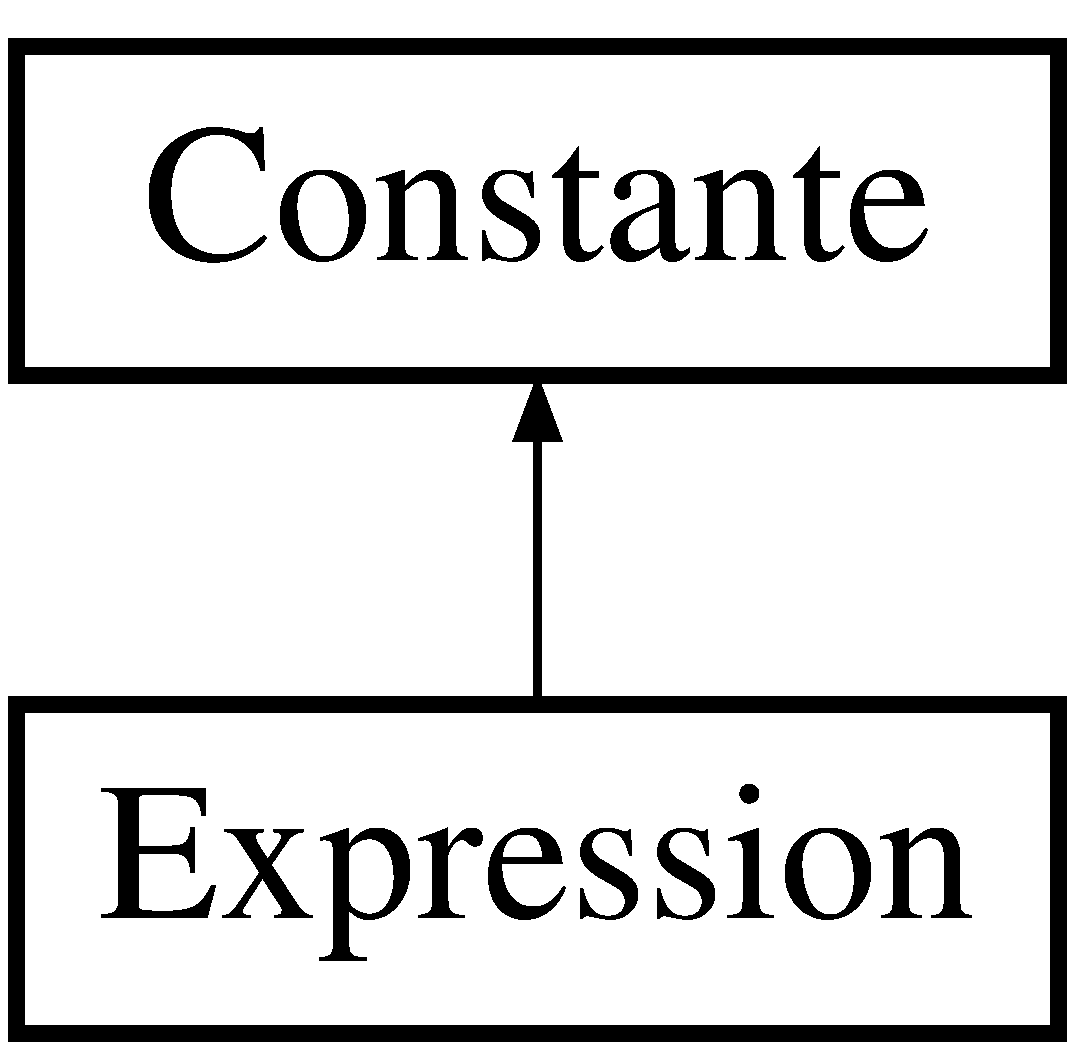
\includegraphics[height=2.000000cm]{class_expression}
\end{center}
\end{figure}
\subsection*{Public Member Functions}
\begin{DoxyCompactItemize}
\item 
\hypertarget{class_expression_ac25fb301ae3947c964a4da9a95883e72}{{\bfseries Expression} (Q\-String s)}\label{class_expression_ac25fb301ae3947c964a4da9a95883e72}

\item 
void \hyperlink{class_expression_a82c745bad73c0adf286f893febaf7406}{Afficher} (std\-::ostream \&os=std\-::cout) const 
\begin{DoxyCompactList}\small\item\em Fonction virtuelle pour l'affichage, affichant une constante en console. \end{DoxyCompactList}\item 
double \hyperlink{class_expression_addc8118b94c445af0da80e8e661dfd6a}{Get\-Val} () const 
\begin{DoxyCompactList}\small\item\em Fonction permettant de récupérer la valeur principale des différentes constantes. \end{DoxyCompactList}\item 
double \hyperlink{class_expression_ad602729011040226673d7c1ee94367d9}{Get\-Val\-Bis} () const 
\begin{DoxyCompactList}\small\item\em Fonction permettant de récupérer la valeur secondaire des différentes constantes. \end{DoxyCompactList}\item 
const std\-::string \hyperlink{class_expression_aa96b1065b6d35277b2c30c25966eccfb}{Get\-Type} () const 
\begin{DoxyCompactList}\small\item\em Fonction permettant de récupérer la valeur du type des différentes constantes. \end{DoxyCompactList}\item 
Q\-String \hyperlink{class_expression_ab64fbbad486a07035ada97ae21786db4}{Get\-Q\-String} () const 
\begin{DoxyCompactList}\small\item\em Fonction permettant de transformer une \hyperlink{class_constante}{Constante} en Q\-String. \end{DoxyCompactList}\item 
\hypertarget{class_expression_accbdcaab3d8ffc239d83618d49574733}{void \hyperlink{class_expression_accbdcaab3d8ffc239d83618d49574733}{Set\-Exp} (Q\-String s)}\label{class_expression_accbdcaab3d8ffc239d83618d49574733}

\begin{DoxyCompactList}\small\item\em Fonction permettant de d'affecter la valeur de l'expression. \end{DoxyCompactList}\item 
\hypertarget{class_expression_a9059e6564e7737b2b5f22bb101f0e983}{\hyperlink{class_expression}{Expression} \& {\bfseries operator+} (const \hyperlink{class_entier}{Entier} \&)}\label{class_expression_a9059e6564e7737b2b5f22bb101f0e983}

\item 
\hypertarget{class_expression_aea5f4c261ddbc4933a5e33a309e88aae}{\hyperlink{class_expression}{Expression} \& {\bfseries operator+} (const \hyperlink{class_reel}{Reel} \&)}\label{class_expression_aea5f4c261ddbc4933a5e33a309e88aae}

\item 
\hypertarget{class_expression_aab7cfa2f6b1c04012ce6b054b3c7d67e}{\hyperlink{class_expression}{Expression} \& {\bfseries operator+} (const \hyperlink{class_rationnel}{Rationnel} \&)}\label{class_expression_aab7cfa2f6b1c04012ce6b054b3c7d67e}

\item 
\hypertarget{class_expression_a2ad6d5eebc3f72a578af5d42b0708822}{\hyperlink{class_expression}{Expression} \& {\bfseries operator+} (const \hyperlink{class_complexe}{Complexe} \&)}\label{class_expression_a2ad6d5eebc3f72a578af5d42b0708822}

\item 
\hypertarget{class_expression_a0391f7f7e53f8d1428b924ea2e4c54e4}{\hyperlink{class_expression}{Expression} \& {\bfseries operator+} (\hyperlink{class_expression}{Expression} \&)}\label{class_expression_a0391f7f7e53f8d1428b924ea2e4c54e4}

\item 
\hypertarget{class_expression_a35a71e11411774ec1a29ec727295c5c2}{\hyperlink{class_expression}{Expression} \& {\bfseries operator-\/} (const \hyperlink{class_entier}{Entier} \&)}\label{class_expression_a35a71e11411774ec1a29ec727295c5c2}

\item 
\hypertarget{class_expression_a30114836dc371287d679c87cc516d749}{\hyperlink{class_expression}{Expression} \& {\bfseries operator-\/} (const \hyperlink{class_reel}{Reel} \&)}\label{class_expression_a30114836dc371287d679c87cc516d749}

\item 
\hypertarget{class_expression_a8ea0173138b138ae4758e09b062d2e19}{\hyperlink{class_expression}{Expression} \& {\bfseries operator-\/} (const \hyperlink{class_rationnel}{Rationnel} \&)}\label{class_expression_a8ea0173138b138ae4758e09b062d2e19}

\item 
\hypertarget{class_expression_aaa8249dde39b664ebe61e6d181d0831f}{\hyperlink{class_expression}{Expression} \& {\bfseries operator-\/} (const \hyperlink{class_complexe}{Complexe} \&)}\label{class_expression_aaa8249dde39b664ebe61e6d181d0831f}

\item 
\hypertarget{class_expression_ad52c4607568b74ce67473ddbfa4249b9}{\hyperlink{class_expression}{Expression} \& {\bfseries operator-\/} (\hyperlink{class_expression}{Expression} \&)}\label{class_expression_ad52c4607568b74ce67473ddbfa4249b9}

\item 
\hypertarget{class_expression_ae9b8bdd91b8669637b556c31de62fb34}{\hyperlink{class_expression}{Expression} \& {\bfseries operator$\ast$} (const \hyperlink{class_entier}{Entier} \&)}\label{class_expression_ae9b8bdd91b8669637b556c31de62fb34}

\item 
\hypertarget{class_expression_a1e0b5b04b6d1e431c7b1071f28853458}{\hyperlink{class_expression}{Expression} \& {\bfseries operator$\ast$} (const \hyperlink{class_reel}{Reel} \&)}\label{class_expression_a1e0b5b04b6d1e431c7b1071f28853458}

\item 
\hypertarget{class_expression_a5823d9314483c0bc1cb8c8ccde63f5f6}{\hyperlink{class_expression}{Expression} \& {\bfseries operator$\ast$} (const \hyperlink{class_rationnel}{Rationnel} \&)}\label{class_expression_a5823d9314483c0bc1cb8c8ccde63f5f6}

\item 
\hypertarget{class_expression_adc2d8cf609d1435fec8344d43991a3d4}{\hyperlink{class_expression}{Expression} \& {\bfseries operator$\ast$} (const \hyperlink{class_complexe}{Complexe} \&)}\label{class_expression_adc2d8cf609d1435fec8344d43991a3d4}

\item 
\hypertarget{class_expression_af80f07ddc178724afcd0f1be7ae8cc1f}{\hyperlink{class_expression}{Expression} \& {\bfseries operator$\ast$} (\hyperlink{class_expression}{Expression} \&)}\label{class_expression_af80f07ddc178724afcd0f1be7ae8cc1f}

\item 
\hypertarget{class_expression_afe16f94062884e326bf9c1c61e21e0ac}{\hyperlink{class_expression}{Expression} \& {\bfseries operator/} (const \hyperlink{class_entier}{Entier} \&)}\label{class_expression_afe16f94062884e326bf9c1c61e21e0ac}

\item 
\hypertarget{class_expression_abf12b51b3587e7dec24ab1d8a218a251}{\hyperlink{class_expression}{Expression} \& {\bfseries operator/} (const \hyperlink{class_reel}{Reel} \&)}\label{class_expression_abf12b51b3587e7dec24ab1d8a218a251}

\item 
\hypertarget{class_expression_aac26e92c371f49f8a581ebfd1223dd4a}{\hyperlink{class_expression}{Expression} \& {\bfseries operator/} (const \hyperlink{class_rationnel}{Rationnel} \&)}\label{class_expression_aac26e92c371f49f8a581ebfd1223dd4a}

\item 
\hypertarget{class_expression_ae75f2ec143a40d53ee1b7fa1c1f7c80f}{\hyperlink{class_expression}{Expression} \& {\bfseries operator/} (const \hyperlink{class_complexe}{Complexe} \&)}\label{class_expression_ae75f2ec143a40d53ee1b7fa1c1f7c80f}

\item 
\hypertarget{class_expression_afdf66c304b67b599336d832b2dde2f92}{\hyperlink{class_expression}{Expression} \& {\bfseries operator/} (\hyperlink{class_expression}{Expression} \&)}\label{class_expression_afdf66c304b67b599336d832b2dde2f92}

\item 
\hypertarget{class_expression_abd5043859ed768c2230a5296f5ca1020}{\hyperlink{class_expression}{Expression} \& {\bfseries cos\-Fonction} (std\-::string)}\label{class_expression_abd5043859ed768c2230a5296f5ca1020}

\item 
\hypertarget{class_expression_a344158f97bc06689c458000eea5743e1}{\hyperlink{class_expression}{Expression} \& {\bfseries sin\-Fonction} (std\-::string)}\label{class_expression_a344158f97bc06689c458000eea5743e1}

\item 
\hypertarget{class_expression_a1fa57ac3a29bdb723371de604cfb5bdc}{\hyperlink{class_expression}{Expression} \& {\bfseries tan\-Fonction} (std\-::string)}\label{class_expression_a1fa57ac3a29bdb723371de604cfb5bdc}

\item 
\hypertarget{class_expression_a23e005f6f25a9768302a1337c4f074f1}{\hyperlink{class_expression}{Expression} \& {\bfseries cosh\-Fonction} (std\-::string)}\label{class_expression_a23e005f6f25a9768302a1337c4f074f1}

\item 
\hypertarget{class_expression_a6eae473ce30bd7f1b03961be4a1c1103}{\hyperlink{class_expression}{Expression} \& {\bfseries sinh\-Fonction} (std\-::string)}\label{class_expression_a6eae473ce30bd7f1b03961be4a1c1103}

\item 
\hypertarget{class_expression_a92f8d74008d1cb0d44bd705463a7416a}{\hyperlink{class_expression}{Expression} \& {\bfseries tanh\-Fonction} (std\-::string)}\label{class_expression_a92f8d74008d1cb0d44bd705463a7416a}

\item 
\hypertarget{class_expression_affde75e11b8700af3abcd47007a508fa}{\hyperlink{class_expression}{Expression} \& {\bfseries pow\-Fonction} (const \hyperlink{class_entier}{Entier} \&)}\label{class_expression_affde75e11b8700af3abcd47007a508fa}

\item 
\hypertarget{class_expression_a2fb3923dfcc37b04343ceb1007d24d6b}{\hyperlink{class_expression}{Expression} \& {\bfseries pow\-Fonction} (const \hyperlink{class_reel}{Reel} \&)}\label{class_expression_a2fb3923dfcc37b04343ceb1007d24d6b}

\item 
\hypertarget{class_expression_a0e76639cff34bad17689d4a5107dc176}{\hyperlink{class_expression}{Expression} \& {\bfseries pow\-Fonction} (const \hyperlink{class_rationnel}{Rationnel} \&)}\label{class_expression_a0e76639cff34bad17689d4a5107dc176}

\item 
\hypertarget{class_expression_a48839cd4843fe09e95c2dc4dff18106e}{\hyperlink{class_expression}{Expression} \& {\bfseries pow\-Fonction} (const \hyperlink{class_complexe}{Complexe} \&)}\label{class_expression_a48839cd4843fe09e95c2dc4dff18106e}

\item 
\hypertarget{class_expression_aea48c6f6091bf8b2b99a1845419bc0dc}{\hyperlink{class_expression}{Expression} \& {\bfseries pow\-Fonction} (\hyperlink{class_expression}{Expression} \&)}\label{class_expression_aea48c6f6091bf8b2b99a1845419bc0dc}

\end{DoxyCompactItemize}


\subsection{Detailed Description}
Classe permettant de gérer le type expression pouvant être évaluer à tout moment. 

Le type expression est une Chaîne de caractères déclaré entre quote, pouvant reporter un calcule. Ce dernier ne peut-\/être réalisé qu'à travers la fonction eval. 

\subsection{Member Function Documentation}
\hypertarget{class_expression_a82c745bad73c0adf286f893febaf7406}{\index{Expression@{Expression}!Afficher@{Afficher}}
\index{Afficher@{Afficher}!Expression@{Expression}}
\subsubsection[{Afficher}]{\setlength{\rightskip}{0pt plus 5cm}void Expression\-::\-Afficher (
\begin{DoxyParamCaption}
\item[{std\-::ostream \&}]{os = {\ttfamily std\-:\-:cout}}
\end{DoxyParamCaption}
) const\hspace{0.3cm}{\ttfamily [inline]}, {\ttfamily [virtual]}}}\label{class_expression_a82c745bad73c0adf286f893febaf7406}


Fonction virtuelle pour l'affichage, affichant une constante en console. 


\begin{DoxyParams}{Parameters}
{\em os} & flux d'affichage \\
\hline
\end{DoxyParams}


Implements \hyperlink{class_constante_af3be055efee6c5be81ed6a610dbe2082}{Constante}.

\hypertarget{class_expression_ab64fbbad486a07035ada97ae21786db4}{\index{Expression@{Expression}!Get\-Q\-String@{Get\-Q\-String}}
\index{Get\-Q\-String@{Get\-Q\-String}!Expression@{Expression}}
\subsubsection[{Get\-Q\-String}]{\setlength{\rightskip}{0pt plus 5cm}Q\-String Expression\-::\-Get\-Q\-String (
\begin{DoxyParamCaption}
{}
\end{DoxyParamCaption}
) const\hspace{0.3cm}{\ttfamily [inline]}, {\ttfamily [virtual]}}}\label{class_expression_ab64fbbad486a07035ada97ae21786db4}


Fonction permettant de transformer une \hyperlink{class_constante}{Constante} en Q\-String. 

\begin{DoxyReturn}{Returns}
Q\-String. 
\end{DoxyReturn}


Implements \hyperlink{class_constante_a7c3edb9082492c95eb319da3d42bb7a4}{Constante}.

\hypertarget{class_expression_aa96b1065b6d35277b2c30c25966eccfb}{\index{Expression@{Expression}!Get\-Type@{Get\-Type}}
\index{Get\-Type@{Get\-Type}!Expression@{Expression}}
\subsubsection[{Get\-Type}]{\setlength{\rightskip}{0pt plus 5cm}const std\-::string Expression\-::\-Get\-Type (
\begin{DoxyParamCaption}
{}
\end{DoxyParamCaption}
) const\hspace{0.3cm}{\ttfamily [inline]}, {\ttfamily [virtual]}}}\label{class_expression_aa96b1065b6d35277b2c30c25966eccfb}


Fonction permettant de récupérer la valeur du type des différentes constantes. 

\begin{DoxyReturn}{Returns}
String. 
\end{DoxyReturn}


Implements \hyperlink{class_constante_a2f716a85b9b519b7bbf8ed8d997f66d3}{Constante}.

\hypertarget{class_expression_addc8118b94c445af0da80e8e661dfd6a}{\index{Expression@{Expression}!Get\-Val@{Get\-Val}}
\index{Get\-Val@{Get\-Val}!Expression@{Expression}}
\subsubsection[{Get\-Val}]{\setlength{\rightskip}{0pt plus 5cm}double Expression\-::\-Get\-Val (
\begin{DoxyParamCaption}
{}
\end{DoxyParamCaption}
) const\hspace{0.3cm}{\ttfamily [inline]}, {\ttfamily [virtual]}}}\label{class_expression_addc8118b94c445af0da80e8e661dfd6a}


Fonction permettant de récupérer la valeur principale des différentes constantes. 

\begin{DoxyReturn}{Returns}
Double. 
\end{DoxyReturn}


Implements \hyperlink{class_constante_af88eb444ed659cc6bb2f9571326a9eb1}{Constante}.

\hypertarget{class_expression_ad602729011040226673d7c1ee94367d9}{\index{Expression@{Expression}!Get\-Val\-Bis@{Get\-Val\-Bis}}
\index{Get\-Val\-Bis@{Get\-Val\-Bis}!Expression@{Expression}}
\subsubsection[{Get\-Val\-Bis}]{\setlength{\rightskip}{0pt plus 5cm}double Expression\-::\-Get\-Val\-Bis (
\begin{DoxyParamCaption}
{}
\end{DoxyParamCaption}
) const\hspace{0.3cm}{\ttfamily [inline]}, {\ttfamily [virtual]}}}\label{class_expression_ad602729011040226673d7c1ee94367d9}


Fonction permettant de récupérer la valeur secondaire des différentes constantes. 

\begin{DoxyReturn}{Returns}
Double. 
\end{DoxyReturn}


Implements \hyperlink{class_constante_aa0602d62c04f28f7bda68723f5dbc48b}{Constante}.



The documentation for this class was generated from the following files\-:\begin{DoxyCompactItemize}
\item 
\hyperlink{constante_8h}{constante.\-h}\item 
constante\-Op\-Div.\-cpp\item 
constante\-Op\-Moins.\-cpp\item 
constante\-Op\-Mult.\-cpp\item 
constante\-Op\-Plus.\-cpp\item 
constante\-Op\-Pow.\-cpp\item 
operateurs\-Unaires.\-cpp\end{DoxyCompactItemize}

\hypertarget{class_gardien}{\section{Gardien Class Reference}
\label{class_gardien}\index{Gardien@{Gardien}}
}


Classe permettant d'empiler et de dépiler les \hyperlink{class_memento_stock}{Memento\-Stock} \& \hyperlink{class_memento_aff}{Memento\-Aff}.  




{\ttfamily \#include $<$memento.\-h$>$}

\subsection*{Public Member Functions}
\begin{DoxyCompactItemize}
\item 
\hypertarget{class_gardien_a25ff2936955eb98a8eef1fbe4dc0b9d0}{void {\bfseries Ajouter\-Memento} (\hyperlink{class_memento_stock}{Memento\-Stock} $\ast$m)}\label{class_gardien_a25ff2936955eb98a8eef1fbe4dc0b9d0}

\item 
\hypertarget{class_gardien_a01fe8e7e99114ecc5979a9109001c24d}{\hyperlink{class_memento_stock}{Memento\-Stock} $\ast$ {\bfseries Annuler\-Stock} ()}\label{class_gardien_a01fe8e7e99114ecc5979a9109001c24d}

\item 
\hypertarget{class_gardien_a106f068a93a38b146201d6dc8d9b06e6}{\hyperlink{class_memento_stock}{Memento\-Stock} $\ast$ {\bfseries Retablir\-Stock} ()}\label{class_gardien_a106f068a93a38b146201d6dc8d9b06e6}

\item 
\hypertarget{class_gardien_ab24502a38d3078c3c24510e13a6486ee}{void {\bfseries Ajouter\-Memento} (\hyperlink{class_memento_aff}{Memento\-Aff} $\ast$m)}\label{class_gardien_ab24502a38d3078c3c24510e13a6486ee}

\item 
\hypertarget{class_gardien_ad607200bff6e2b690ab5b065c77cbd7b}{\hyperlink{class_memento_aff}{Memento\-Aff} $\ast$ {\bfseries Annuler\-Aff} ()}\label{class_gardien_ad607200bff6e2b690ab5b065c77cbd7b}

\item 
\hypertarget{class_gardien_af2bee95e5eee42060dd738ad73187b5c}{\hyperlink{class_memento_aff}{Memento\-Aff} $\ast$ {\bfseries Retablir\-Aff} ()}\label{class_gardien_af2bee95e5eee42060dd738ad73187b5c}

\end{DoxyCompactItemize}
\subsection*{Static Public Member Functions}
\begin{DoxyCompactItemize}
\item 
\hypertarget{class_gardien_a4b27ca18c44dabd54b0c917d0507d6ba}{static \hyperlink{class_gardien}{Gardien} $\ast$ {\bfseries Get\-Instance} ()}\label{class_gardien_a4b27ca18c44dabd54b0c917d0507d6ba}

\item 
\hypertarget{class_gardien_a0fb33b3613867d0ee2dee53b73faeec6}{static void {\bfseries Detruire\-Instance} ()}\label{class_gardien_a0fb33b3613867d0ee2dee53b73faeec6}

\end{DoxyCompactItemize}


\subsection{Detailed Description}
Classe permettant d'empiler et de dépiler les \hyperlink{class_memento_stock}{Memento\-Stock} \& \hyperlink{class_memento_aff}{Memento\-Aff}. 

Cette classe sert à sauvegarder les mementos des deux piles, elle peut rétablir ou annuler un état. 

The documentation for this class was generated from the following files\-:\begin{DoxyCompactItemize}
\item 
\hyperlink{memento_8h}{memento.\-h}\item 
memento.\-cpp\end{DoxyCompactItemize}

\hypertarget{class_ui_1_1_main_window}{\section{Ui\-:\-:Main\-Window Class Reference}
\label{class_ui_1_1_main_window}\index{Ui\-::\-Main\-Window@{Ui\-::\-Main\-Window}}
}
Inheritance diagram for Ui\-:\-:Main\-Window\-:\begin{figure}[H]
\begin{center}
\leavevmode
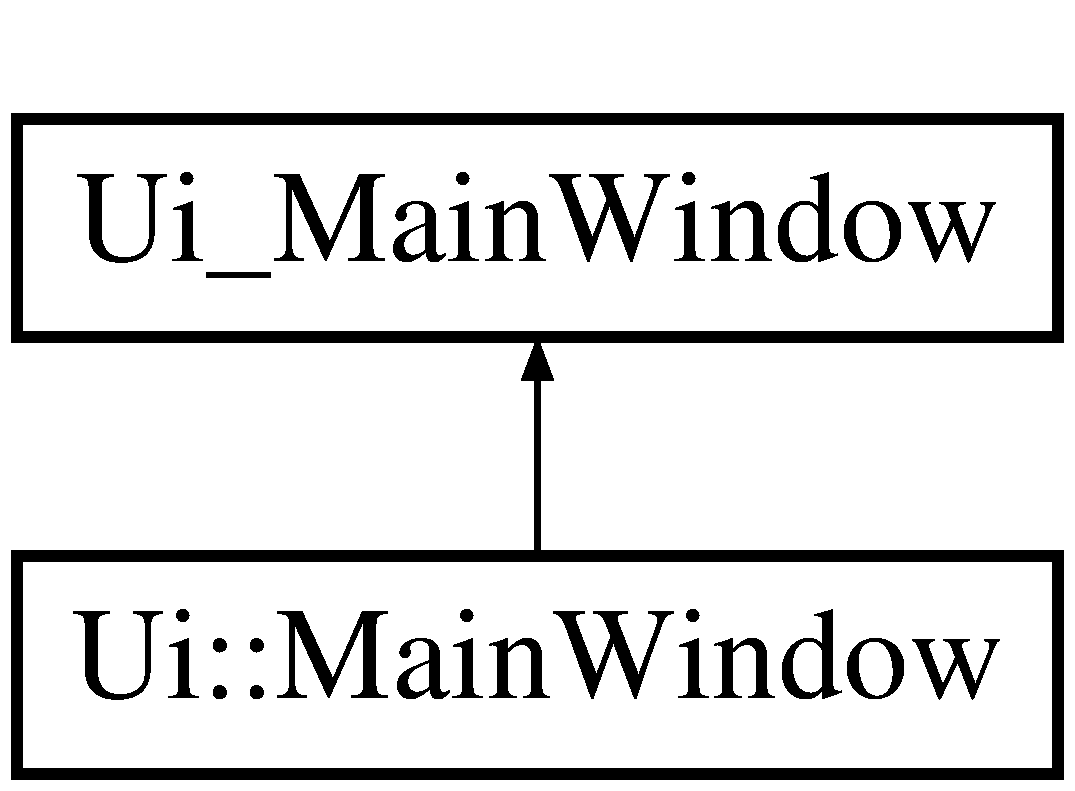
\includegraphics[height=2.000000cm]{class_ui_1_1_main_window}
\end{center}
\end{figure}
\subsection*{Additional Inherited Members}


The documentation for this class was generated from the following file\-:\begin{DoxyCompactItemize}
\item 
ui\-\_\-mainwindow.\-h\end{DoxyCompactItemize}

\hypertarget{class_main_window}{\section{Main\-Window Class Reference}
\label{class_main_window}\index{Main\-Window@{Main\-Window}}
}
\subsection*{Public Slots}
\begin{DoxyCompactItemize}
\item 
\hypertarget{class_main_window_a85c6273206499c1a041b6d532b2224d5}{void {\bfseries Num1\-Press} ()}\label{class_main_window_a85c6273206499c1a041b6d532b2224d5}

\item 
\hypertarget{class_main_window_a29719cefd3c330c215fd445d28f160c1}{void {\bfseries Num2\-Press} ()}\label{class_main_window_a29719cefd3c330c215fd445d28f160c1}

\item 
\hypertarget{class_main_window_a87992b9459776c9a888552d50c5f056f}{void {\bfseries Num3\-Press} ()}\label{class_main_window_a87992b9459776c9a888552d50c5f056f}

\item 
\hypertarget{class_main_window_a30a12a00bf2e07572f4246689c0f28fd}{void {\bfseries Num4\-Press} ()}\label{class_main_window_a30a12a00bf2e07572f4246689c0f28fd}

\item 
\hypertarget{class_main_window_a3c7fbf12f84ed2f3626110f916b0b2ae}{void {\bfseries Num5\-Press} ()}\label{class_main_window_a3c7fbf12f84ed2f3626110f916b0b2ae}

\item 
\hypertarget{class_main_window_adbce6964b135381217ecb1743d3e4aa9}{void {\bfseries Num6\-Press} ()}\label{class_main_window_adbce6964b135381217ecb1743d3e4aa9}

\item 
\hypertarget{class_main_window_ae6f603a01e255e33224db1b19b78759f}{void {\bfseries Num7\-Press} ()}\label{class_main_window_ae6f603a01e255e33224db1b19b78759f}

\item 
\hypertarget{class_main_window_a6e87ab64100597c39f816aa98b13b0ac}{void {\bfseries Num8\-Press} ()}\label{class_main_window_a6e87ab64100597c39f816aa98b13b0ac}

\item 
\hypertarget{class_main_window_a0a93067c07a5b7c7db871328cc0c902d}{void {\bfseries Num9\-Press} ()}\label{class_main_window_a0a93067c07a5b7c7db871328cc0c902d}

\item 
\hypertarget{class_main_window_a0440904b9a671b668843b425d3881edd}{void {\bfseries Num0\-Press} ()}\label{class_main_window_a0440904b9a671b668843b425d3881edd}

\item 
\hypertarget{class_main_window_a8b0963e9fa883ef0770ba2ad1076d49a}{void {\bfseries Del\-Press} ()}\label{class_main_window_a8b0963e9fa883ef0770ba2ad1076d49a}

\item 
\hypertarget{class_main_window_ae277e1c40950272d2485a8aab226d592}{void {\bfseries Coma\-Press} ()}\label{class_main_window_ae277e1c40950272d2485a8aab226d592}

\item 
\hypertarget{class_main_window_a320eadd68e54c4c6afa6fc4b94022742}{void {\bfseries Cmplx\-Press} ()}\label{class_main_window_a320eadd68e54c4c6afa6fc4b94022742}

\item 
\hypertarget{class_main_window_a55315d728897bf15c6fccd07744f275a}{void {\bfseries Expr\-Press} ()}\label{class_main_window_a55315d728897bf15c6fccd07744f275a}

\item 
\hypertarget{class_main_window_a524870a90ed045d8c644d15c378b1143}{void {\bfseries Div\-Press} ()}\label{class_main_window_a524870a90ed045d8c644d15c378b1143}

\item 
\hypertarget{class_main_window_a0f0b546be0aed132588e705164f8331c}{void {\bfseries Mod\-Press} ()}\label{class_main_window_a0f0b546be0aed132588e705164f8331c}

\item 
\hypertarget{class_main_window_ac584aa6ec3b22898ce17b96e6562c3b2}{void {\bfseries Plus\-Press} ()}\label{class_main_window_ac584aa6ec3b22898ce17b96e6562c3b2}

\item 
\hypertarget{class_main_window_a582bfb70dbb6ec053ecefa291308e432}{void {\bfseries Moins\-Press} ()}\label{class_main_window_a582bfb70dbb6ec053ecefa291308e432}

\item 
\hypertarget{class_main_window_a1b2412bdcdd9bfa2b5d199e0f0adc27f}{void {\bfseries Mult\-Press} ()}\label{class_main_window_a1b2412bdcdd9bfa2b5d199e0f0adc27f}

\item 
\hypertarget{class_main_window_ab9c019705c77a24ba816c5a0cc625120}{void {\bfseries Fact\-Press} ()}\label{class_main_window_ab9c019705c77a24ba816c5a0cc625120}

\item 
\hypertarget{class_main_window_a0ea62adb218277a6a0fcd8dac7f6a696}{void {\bfseries Sign\-Press} ()}\label{class_main_window_a0ea62adb218277a6a0fcd8dac7f6a696}

\item 
\hypertarget{class_main_window_ac20e692a02e6df29d716c8c8aafb69df}{void {\bfseries Sqr\-Press} ()}\label{class_main_window_ac20e692a02e6df29d716c8c8aafb69df}

\item 
\hypertarget{class_main_window_a4f2f3431c0d564f79985b3aedbbba25a}{void {\bfseries Cube\-Press} ()}\label{class_main_window_a4f2f3431c0d564f79985b3aedbbba25a}

\item 
\hypertarget{class_main_window_a4682d9dfeb34ca2591388cf6768be17d}{void {\bfseries Sqrt\-Press} ()}\label{class_main_window_a4682d9dfeb34ca2591388cf6768be17d}

\item 
\hypertarget{class_main_window_ad84b1c04bdb222493d4b19cff132dfb1}{void {\bfseries Inv\-Press} ()}\label{class_main_window_ad84b1c04bdb222493d4b19cff132dfb1}

\item 
\hypertarget{class_main_window_a63718029769796e30e307733bc5c90a6}{void {\bfseries Entrer\-Press} ()}\label{class_main_window_a63718029769796e30e307733bc5c90a6}

\item 
\hypertarget{class_main_window_aac0bbc34c283cbf7dc25cd10c24ff9ba}{void {\bfseries Menu\-Complexe} ()}\label{class_main_window_aac0bbc34c283cbf7dc25cd10c24ff9ba}

\item 
\hypertarget{class_main_window_aed617b8e29e044e378a4ad59b4d1b9eb}{void {\bfseries Menu\-Entier} ()}\label{class_main_window_aed617b8e29e044e378a4ad59b4d1b9eb}

\item 
\hypertarget{class_main_window_adced4a05256a0219fc7694ce82f19dac}{void {\bfseries Menu\-Reel} ()}\label{class_main_window_adced4a05256a0219fc7694ce82f19dac}

\item 
\hypertarget{class_main_window_ac6b74e4dac6f2c2b2052b0d0623ccaa4}{void {\bfseries Menu\-Rationnel} ()}\label{class_main_window_ac6b74e4dac6f2c2b2052b0d0623ccaa4}

\item 
\hypertarget{class_main_window_aba12ee4166b7b369efe36b2decc79054}{void {\bfseries Menu\-Clavier} ()}\label{class_main_window_aba12ee4166b7b369efe36b2decc79054}

\item 
\hypertarget{class_main_window_a1cdce1fa732ad43085a0803c2eb950cc}{void {\bfseries Menu\-Degres} ()}\label{class_main_window_a1cdce1fa732ad43085a0803c2eb950cc}

\item 
\hypertarget{class_main_window_a1a5c21544c6e3dbd5dfce7d1d0e09951}{void {\bfseries Menu\-Radians} ()}\label{class_main_window_a1a5c21544c6e3dbd5dfce7d1d0e09951}

\item 
\hypertarget{class_main_window_a686d78951551e85e142b8b431c5d2ac3}{void {\bfseries Annuler\-Press} ()}\label{class_main_window_a686d78951551e85e142b8b431c5d2ac3}

\item 
\hypertarget{class_main_window_a36a0407a32d14ae1c0b385e3b71620ce}{void {\bfseries Retablir\-Press} ()}\label{class_main_window_a36a0407a32d14ae1c0b385e3b71620ce}

\item 
\hypertarget{class_main_window_abd9bd07b87b11515b778e55ae60e0637}{void {\bfseries Swap\-Press} ()}\label{class_main_window_abd9bd07b87b11515b778e55ae60e0637}

\item 
\hypertarget{class_main_window_a4d9f625070950f2d1cf97d36c63ca8f2}{void {\bfseries Clear\-Press} ()}\label{class_main_window_a4d9f625070950f2d1cf97d36c63ca8f2}

\item 
\hypertarget{class_main_window_af27fca54c0d219a14b59ea64bbe5b235}{void {\bfseries Dup\-Press} ()}\label{class_main_window_af27fca54c0d219a14b59ea64bbe5b235}

\item 
\hypertarget{class_main_window_ad02c1a38753f72e73e67403e466a8318}{void {\bfseries Drop\-Press} ()}\label{class_main_window_ad02c1a38753f72e73e67403e466a8318}

\item 
\hypertarget{class_main_window_a5776a67da8999b2303d9a03bfcbc68c7}{void {\bfseries Sum\-Press} ()}\label{class_main_window_a5776a67da8999b2303d9a03bfcbc68c7}

\item 
\hypertarget{class_main_window_a1e2b4f4827437fa028813ba800258ea5}{void {\bfseries Mean\-Press} ()}\label{class_main_window_a1e2b4f4827437fa028813ba800258ea5}

\item 
\hypertarget{class_main_window_a5d3baaa225ee860a2cb2b28f0ff34e48}{void {\bfseries Eval\-Press} ()}\label{class_main_window_a5d3baaa225ee860a2cb2b28f0ff34e48}

\item 
\hypertarget{class_main_window_ab740fba06e85bec4d9aeea3a6d6699bc}{void {\bfseries Cos\-Press} ()}\label{class_main_window_ab740fba06e85bec4d9aeea3a6d6699bc}

\item 
\hypertarget{class_main_window_a148681088d29ec647bbdf29a79a437ae}{void {\bfseries Sin\-Press} ()}\label{class_main_window_a148681088d29ec647bbdf29a79a437ae}

\item 
\hypertarget{class_main_window_abeb6a2d25072c734455f6674a168e9be}{void {\bfseries Tan\-Press} ()}\label{class_main_window_abeb6a2d25072c734455f6674a168e9be}

\item 
\hypertarget{class_main_window_a9b657c9aa7a088a1601907474f190f9e}{void {\bfseries Cosh\-Press} ()}\label{class_main_window_a9b657c9aa7a088a1601907474f190f9e}

\item 
\hypertarget{class_main_window_aa0d0be9f69773c1609fbfeac9e3eb677}{void {\bfseries Sinh\-Press} ()}\label{class_main_window_aa0d0be9f69773c1609fbfeac9e3eb677}

\item 
\hypertarget{class_main_window_a143f121b2e2322a4e2c330ef8a6317dc}{void {\bfseries Tanh\-Press} ()}\label{class_main_window_a143f121b2e2322a4e2c330ef8a6317dc}

\item 
\hypertarget{class_main_window_aab79909a97d1753ee596cc7c3ba55cbd}{void {\bfseries Pow\-Press} ()}\label{class_main_window_aab79909a97d1753ee596cc7c3ba55cbd}

\item 
\hypertarget{class_main_window_aabe721284a99f3cd8cb251bc2c532a14}{void {\bfseries x\-Press} ()}\label{class_main_window_aabe721284a99f3cd8cb251bc2c532a14}

\item 
\hypertarget{class_main_window_a2007b7dbd387d5d3d1d97ec0f1459617}{void {\bfseries x\-Egal\-Press} ()}\label{class_main_window_a2007b7dbd387d5d3d1d97ec0f1459617}

\end{DoxyCompactItemize}
\subsection*{Public Member Functions}
\begin{DoxyCompactItemize}
\item 
\hypertarget{class_main_window_a8b244be8b7b7db1b08de2a2acb9409db}{{\bfseries Main\-Window} (Q\-Widget $\ast$parent=0)}\label{class_main_window_a8b244be8b7b7db1b08de2a2acb9409db}

\item 
\hypertarget{class_main_window_ac78de1f17d1e936e0b5efa2b7d0e5804}{void {\bfseries Affichage\-Ecran} ()}\label{class_main_window_ac78de1f17d1e936e0b5efa2b7d0e5804}

\item 
\hypertarget{class_main_window_a19564c9faee3e04539c431230b0beb03}{void {\bfseries Init\-Param} ()}\label{class_main_window_a19564c9faee3e04539c431230b0beb03}

\item 
\hypertarget{class_main_window_af644382f0604f07829f789f2c807e06f}{void {\bfseries M\-A\-J\-Param} ()}\label{class_main_window_af644382f0604f07829f789f2c807e06f}

\item 
\hypertarget{class_main_window_a6cd67d43f112d2035d240b4f3f219b75}{void {\bfseries Application\-Menu} ()}\label{class_main_window_a6cd67d43f112d2035d240b4f3f219b75}

\item 
\hypertarget{class_main_window_ae7de56fcd961e099f6df85baab3b8022}{void {\bfseries Traitement\-Erreur} (Q\-String)}\label{class_main_window_ae7de56fcd961e099f6df85baab3b8022}

\end{DoxyCompactItemize}


The documentation for this class was generated from the following files\-:\begin{DoxyCompactItemize}
\item 
mainwindow.\-h\item 
affichage\-Autre.\-cpp\item 
affichage\-Num.\-cpp\item 
affichage\-Op.\-cpp\item 
mainwindow.\-cpp\item 
menu.\-cpp\item 
pile\-Op.\-cpp\end{DoxyCompactItemize}

\hypertarget{class_memento_aff}{\section{Memento\-Aff Class Reference}
\label{class_memento_aff}\index{Memento\-Aff@{Memento\-Aff}}
}


Classe permettant d'annuler et de rétablir un état de \hyperlink{class_pile_affichage}{Pile\-Affichage}.  




{\ttfamily \#include $<$memento.\-h$>$}

\subsection*{Public Member Functions}
\begin{DoxyCompactItemize}
\item 
\hypertarget{class_memento_aff_a0286b7961cf51f82ca2241b7aa8a9d3b}{{\bfseries Memento\-Aff} (std\-::deque$<$ Q\-String $>$ state)}\label{class_memento_aff_a0286b7961cf51f82ca2241b7aa8a9d3b}

\item 
\hypertarget{class_memento_aff_ab2e4c86ddea4e8da29e7b3410c860c97}{std\-::deque$<$ Q\-String $>$ {\bfseries Get\-Etat\-Sauve} () const }\label{class_memento_aff_ab2e4c86ddea4e8da29e7b3410c860c97}

\item 
\hypertarget{class_memento_aff_ab71f491485e0515fb09740c7ace4acfc}{void {\bfseries test} ()}\label{class_memento_aff_ab71f491485e0515fb09740c7ace4acfc}

\end{DoxyCompactItemize}


\subsection{Detailed Description}
Classe permettant d'annuler et de rétablir un état de \hyperlink{class_pile_affichage}{Pile\-Affichage}. 

Cette classe sauvegarde à chaque changement le contenu de \hyperlink{class_pile_affichage}{Pile\-Affichage}. 

The documentation for this class was generated from the following file\-:\begin{DoxyCompactItemize}
\item 
\hyperlink{memento_8h}{memento.\-h}\end{DoxyCompactItemize}

\hypertarget{class_memento_stock}{\section{Memento\-Stock Class Reference}
\label{class_memento_stock}\index{Memento\-Stock@{Memento\-Stock}}
}
\subsection*{Public Member Functions}
\begin{DoxyCompactItemize}
\item 
\hypertarget{class_memento_stock_a31a9bd8576254b31edc21c885d0f0376}{{\bfseries Memento\-Stock} (std\-::deque$<$ \hyperlink{class_constante}{Constante} $\ast$ $>$ state)}\label{class_memento_stock_a31a9bd8576254b31edc21c885d0f0376}

\item 
\hypertarget{class_memento_stock_a14cee296b4fdf6fc421835d6df568100}{std\-::deque$<$ \hyperlink{class_constante}{Constante} $\ast$ $>$ {\bfseries Get\-Etat\-Sauve} () const }\label{class_memento_stock_a14cee296b4fdf6fc421835d6df568100}

\item 
\hypertarget{class_memento_stock_a8ef683ceb96cac42e432ba5845efb88b}{void {\bfseries test} ()}\label{class_memento_stock_a8ef683ceb96cac42e432ba5845efb88b}

\end{DoxyCompactItemize}


The documentation for this class was generated from the following file\-:\begin{DoxyCompactItemize}
\item 
memento.\-h\end{DoxyCompactItemize}

\hypertarget{class_pile_affichage}{\section{Pile\-Affichage Class Reference}
\label{class_pile_affichage}\index{Pile\-Affichage@{Pile\-Affichage}}
}


Classe permettant d'empiler et de dépiler des Q\-String.  




{\ttfamily \#include $<$pile.\-h$>$}

\subsection*{Public Member Functions}
\begin{DoxyCompactItemize}
\item 
\hypertarget{class_pile_affichage_a11bce902517d97e237f99bb36b31bda4}{void {\bfseries Empiler} (Q\-String)}\label{class_pile_affichage_a11bce902517d97e237f99bb36b31bda4}

\item 
\hypertarget{class_pile_affichage_aad2fa732744c8c03ff3f5fa2df874c24}{Q\-String \& {\bfseries Depiler} ()}\label{class_pile_affichage_aad2fa732744c8c03ff3f5fa2df874c24}

\item 
\hypertarget{class_pile_affichage_a5daee2843e955b5f3317ba56e8e99050}{std\-::deque$<$ Q\-String $>$ {\bfseries Get\-Ptr} () const }\label{class_pile_affichage_a5daee2843e955b5f3317ba56e8e99050}

\item 
\hypertarget{class_pile_affichage_a113c2fe93662381bfb58d789123da818}{void {\bfseries Affichage\-Pile} ()}\label{class_pile_affichage_a113c2fe93662381bfb58d789123da818}

\item 
\hypertarget{class_pile_affichage_a04a490c8ab59101a171f1c5cb35a510f}{const Q\-String \& {\bfseries Get\-Val} (int i) const }\label{class_pile_affichage_a04a490c8ab59101a171f1c5cb35a510f}

\item 
\hypertarget{class_pile_affichage_a099c0579bdd31bea548a6fb06e859197}{\hyperlink{class_memento_aff}{Memento\-Aff} $\ast$ {\bfseries Creer\-Memento} ()}\label{class_pile_affichage_a099c0579bdd31bea548a6fb06e859197}

\item 
\hypertarget{class_pile_affichage_aa1eaa41dcfa6317f54f36e3f145dbc4b}{void {\bfseries Charger\-Memento} (\hyperlink{class_memento_aff}{Memento\-Aff} $\ast$mem)}\label{class_pile_affichage_aa1eaa41dcfa6317f54f36e3f145dbc4b}

\item 
\hypertarget{class_pile_affichage_a5768dff9a1bf067cd7ae10567c0dd6a8}{void {\bfseries Swap} (unsigned int, unsigned int)}\label{class_pile_affichage_a5768dff9a1bf067cd7ae10567c0dd6a8}

\item 
\hypertarget{class_pile_affichage_a6676383310776eb66f40ff03095193a3}{void {\bfseries Clear} ()}\label{class_pile_affichage_a6676383310776eb66f40ff03095193a3}

\item 
\hypertarget{class_pile_affichage_a1fbdf1c3578bf2d3d958595f820ae831}{Q\-String {\bfseries Dup} ()}\label{class_pile_affichage_a1fbdf1c3578bf2d3d958595f820ae831}

\item 
\hypertarget{class_pile_affichage_adccff01313daf3c1c7666154549ae4ae}{void {\bfseries Drop} ()}\label{class_pile_affichage_adccff01313daf3c1c7666154549ae4ae}

\item 
\hypertarget{class_pile_affichage_a0cb7b0b675468c8670c6260c3c75d203}{void {\bfseries Save} (std\-::ostream \&os)}\label{class_pile_affichage_a0cb7b0b675468c8670c6260c3c75d203}

\end{DoxyCompactItemize}
\subsection*{Static Public Member Functions}
\begin{DoxyCompactItemize}
\item 
\hypertarget{class_pile_affichage_ae25f21273bf5d03ad1de209b622992a3}{static \hyperlink{class_pile_affichage}{Pile\-Affichage} $\ast$ {\bfseries Get\-Instance} ()}\label{class_pile_affichage_ae25f21273bf5d03ad1de209b622992a3}

\item 
\hypertarget{class_pile_affichage_a1bf96ebc64e812b39f26f821b3a65f4f}{static void {\bfseries Detruire\-Instance} ()}\label{class_pile_affichage_a1bf96ebc64e812b39f26f821b3a65f4f}

\end{DoxyCompactItemize}


\subsection{Detailed Description}
Classe permettant d'empiler et de dépiler des Q\-String. 

Cette classe est l'exacte copie de la \hyperlink{class_pile_stockage}{Pile\-Stockage} mais avec des valeur Q\-String, elle permet une gestion simplifiée de l'affichage. 

The documentation for this class was generated from the following files\-:\begin{DoxyCompactItemize}
\item 
\hyperlink{pile_8h}{pile.\-h}\item 
pile.\-cpp\item 
pile\-Op.\-cpp\end{DoxyCompactItemize}

\hypertarget{class_pile_stockage}{\section{Pile\-Stockage Class Reference}
\label{class_pile_stockage}\index{Pile\-Stockage@{Pile\-Stockage}}
}


Classe permettant d'empiler et de dépiler des pointeurs sur \hyperlink{class_constante}{Constante}.  




{\ttfamily \#include $<$pile.\-h$>$}

\subsection*{Public Member Functions}
\begin{DoxyCompactItemize}
\item 
\hypertarget{class_pile_stockage_abab257876447da78f207a37157f6d3c8}{void {\bfseries Empiler} (\hyperlink{class_constante}{Constante} $\ast$)}\label{class_pile_stockage_abab257876447da78f207a37157f6d3c8}

\item 
\hypertarget{class_pile_stockage_a042c00dd20322ab9c88fcc403ee3af1f}{\hyperlink{class_constante}{Constante} \& {\bfseries Depiler} ()}\label{class_pile_stockage_a042c00dd20322ab9c88fcc403ee3af1f}

\item 
\hypertarget{class_pile_stockage_aa95f27fc7ae06630b58db52faf6316f8}{std\-::deque$<$ \hyperlink{class_constante}{Constante} $\ast$ $>$ {\bfseries Get\-Ptr} () const }\label{class_pile_stockage_aa95f27fc7ae06630b58db52faf6316f8}

\item 
\hypertarget{class_pile_stockage_a27319570899f25a4f0e1f7408ced9127}{void {\bfseries Affichage\-Pile} ()}\label{class_pile_stockage_a27319570899f25a4f0e1f7408ced9127}

\item 
\hypertarget{class_pile_stockage_af558173619e4a4859f740808616a741b}{\hyperlink{class_memento_stock}{Memento\-Stock} $\ast$ {\bfseries Creer\-Memento} ()}\label{class_pile_stockage_af558173619e4a4859f740808616a741b}

\item 
\hypertarget{class_pile_stockage_ab545906e2168095847357f3cbd6c9481}{void {\bfseries Charger\-Memento} (\hyperlink{class_memento_stock}{Memento\-Stock} $\ast$mem)}\label{class_pile_stockage_ab545906e2168095847357f3cbd6c9481}

\item 
\hypertarget{class_pile_stockage_a8e3387a172e0544ecb8e3415da82ef8a}{void {\bfseries Swap} (unsigned int, unsigned int)}\label{class_pile_stockage_a8e3387a172e0544ecb8e3415da82ef8a}

\item 
\hypertarget{class_pile_stockage_a87982d39f9ff25627c7c2ffdb6105048}{void {\bfseries Clear} ()}\label{class_pile_stockage_a87982d39f9ff25627c7c2ffdb6105048}

\item 
\hypertarget{class_pile_stockage_a651e93d46cf89c8145fd51a664a40dda}{\hyperlink{class_constante}{Constante} $\ast$ {\bfseries Dup} ()}\label{class_pile_stockage_a651e93d46cf89c8145fd51a664a40dda}

\item 
\hypertarget{class_pile_stockage_a26f65a5b14708d44d52167f526cebd67}{void {\bfseries Drop} ()}\label{class_pile_stockage_a26f65a5b14708d44d52167f526cebd67}

\item 
\hypertarget{class_pile_stockage_afa26a3bdd4b29a3559a0710b8ab29eba}{\hyperlink{class_constante}{Constante} $\ast$ {\bfseries Sum} (unsigned int)}\label{class_pile_stockage_afa26a3bdd4b29a3559a0710b8ab29eba}

\item 
\hypertarget{class_pile_stockage_a062111e36b1a30b22ccaa8e5e27d0f61}{\hyperlink{class_constante}{Constante} $\ast$ {\bfseries Mean} (unsigned int)}\label{class_pile_stockage_a062111e36b1a30b22ccaa8e5e27d0f61}

\end{DoxyCompactItemize}
\subsection*{Static Public Member Functions}
\begin{DoxyCompactItemize}
\item 
\hypertarget{class_pile_stockage_a92dca143b503c3e55e4a69ad388db464}{static \hyperlink{class_pile_stockage}{Pile\-Stockage} $\ast$ {\bfseries Get\-Instance} ()}\label{class_pile_stockage_a92dca143b503c3e55e4a69ad388db464}

\item 
\hypertarget{class_pile_stockage_a937a1f84b9ab82192b74d6735f691d90}{static void {\bfseries Detruire\-Instance} ()}\label{class_pile_stockage_a937a1f84b9ab82192b74d6735f691d90}

\end{DoxyCompactItemize}


\subsection{Detailed Description}
Classe permettant d'empiler et de dépiler des pointeurs sur \hyperlink{class_constante}{Constante}. 

The documentation for this class was generated from the following files\-:\begin{DoxyCompactItemize}
\item 
\hyperlink{pile_8h}{pile.\-h}\item 
pile.\-cpp\item 
pile\-Op.\-cpp\end{DoxyCompactItemize}

\hypertarget{class_rationnel}{\section{Rationnel Class Reference}
\label{class_rationnel}\index{Rationnel@{Rationnel}}
}


Classe permettant de représenter le type \hyperlink{class_rationnel}{Rationnel}.  




{\ttfamily \#include $<$constante.\-h$>$}

Inheritance diagram for Rationnel\-:\begin{figure}[H]
\begin{center}
\leavevmode
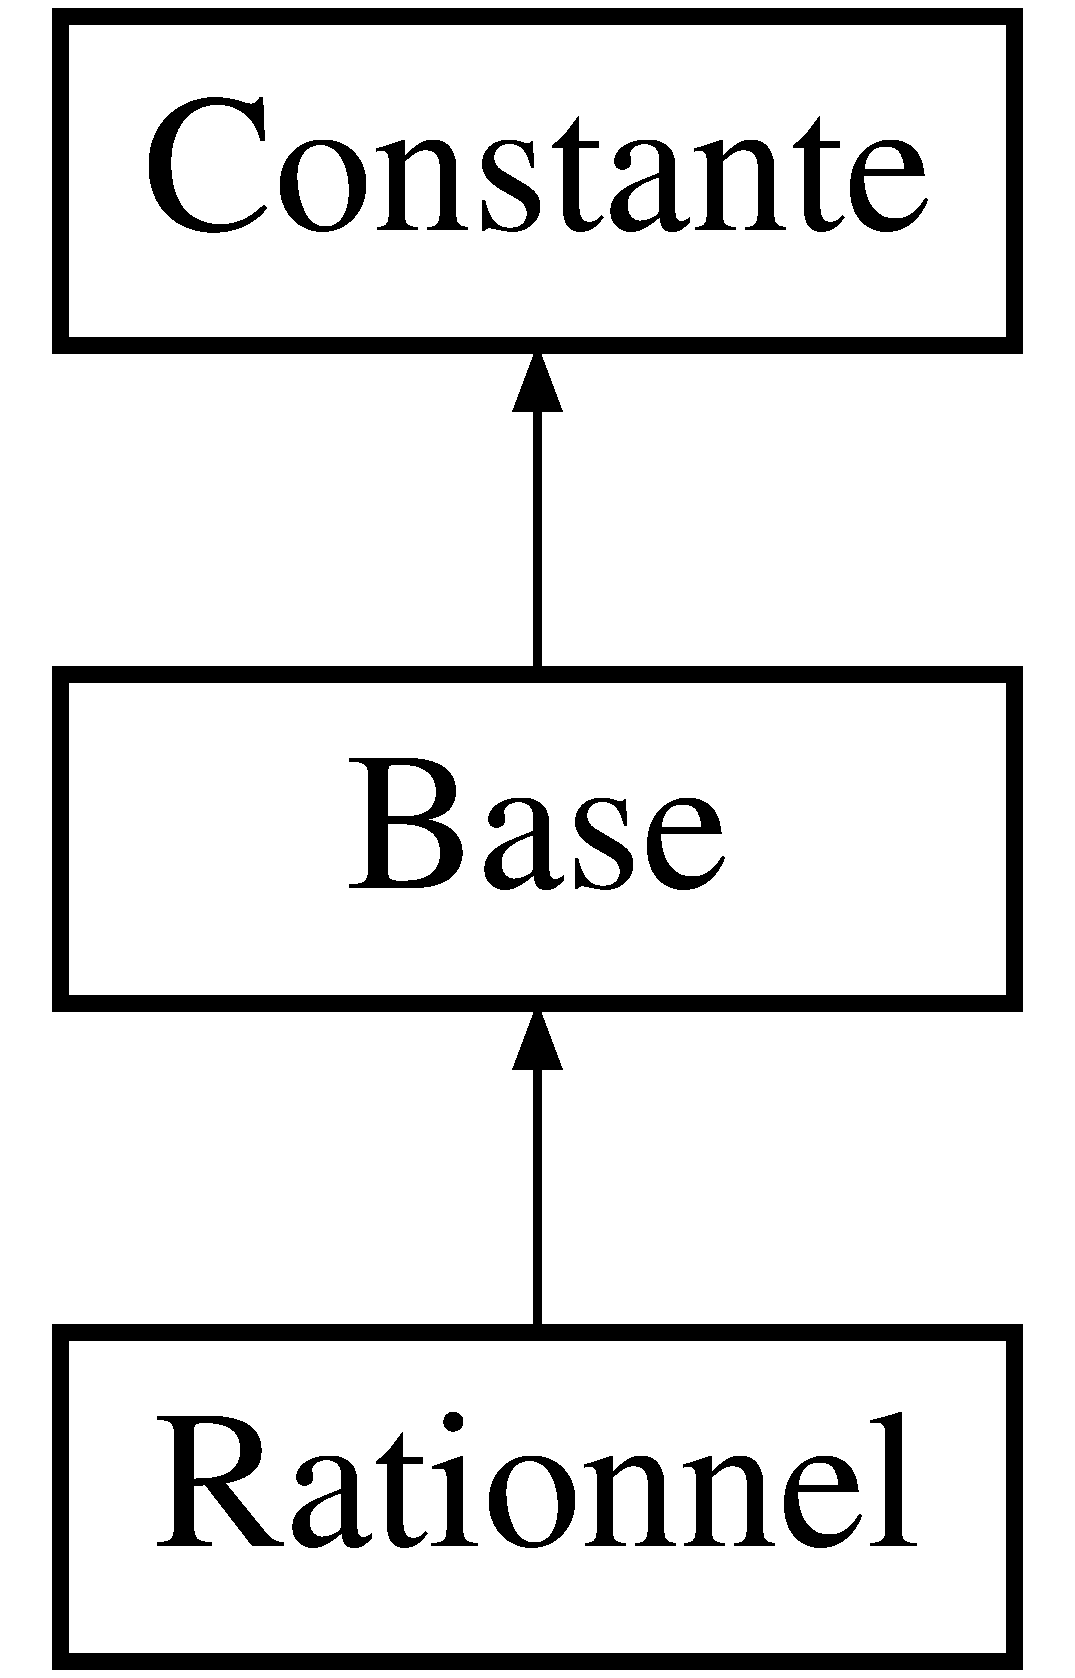
\includegraphics[height=3.000000cm]{class_rationnel}
\end{center}
\end{figure}
\subsection*{Public Member Functions}
\begin{DoxyCompactItemize}
\item 
\hypertarget{class_rationnel_afac9e543020a4611f5c217a01f3c0a7e}{{\bfseries Rationnel} (int num, int den)}\label{class_rationnel_afac9e543020a4611f5c217a01f3c0a7e}

\item 
void \hyperlink{class_rationnel_a52b4a6398d50e630ad76be8be0185f9f}{Afficher} (std\-::ostream \&os=std\-::cout) const 
\begin{DoxyCompactList}\small\item\em Fonction virtuelle pour l'affichage, affichant une constante en console. \end{DoxyCompactList}\item 
double \hyperlink{class_rationnel_a29987744cb2a7631ffa4db708630fe19}{Get\-Val} () const 
\begin{DoxyCompactList}\small\item\em Fonction permettant de récupérer la valeur principale des différentes constantes. \end{DoxyCompactList}\item 
double \hyperlink{class_rationnel_a2403f411e88b3de9f83ad735342e68ec}{Get\-Val\-Bis} () const 
\begin{DoxyCompactList}\small\item\em Fonction permettant de récupérer la valeur secondaire des différentes constantes. \end{DoxyCompactList}\item 
const std\-::string \hyperlink{class_rationnel_a8c04071cda8dbe6f2b13db3e48d1bedb}{Get\-Type} () const 
\begin{DoxyCompactList}\small\item\em Fonction permettant de récupérer la valeur du type des différentes constantes. \end{DoxyCompactList}\item 
Q\-String \hyperlink{class_rationnel_af3d40b73dc2dd7ca6e978fe5ddb0c945}{Get\-Q\-String} () const 
\begin{DoxyCompactList}\small\item\em Fonction permettant de transformer une \hyperlink{class_constante}{Constante} en Q\-String. \end{DoxyCompactList}\item 
\hypertarget{class_rationnel_a07ba81e61e4186ada00f3da12bb24ffc}{double {\bfseries Get\-Num} () const }\label{class_rationnel_a07ba81e61e4186ada00f3da12bb24ffc}

\item 
\hypertarget{class_rationnel_ab2791ae061c2c27af018830c1564fb4c}{double {\bfseries Get\-Den} () const }\label{class_rationnel_ab2791ae061c2c27af018830c1564fb4c}

\item 
\hypertarget{class_rationnel_ab86742d127646fff7096e04c0882e00d}{void \hyperlink{class_rationnel_ab86742d127646fff7096e04c0882e00d}{Simplifier} ()}\label{class_rationnel_ab86742d127646fff7096e04c0882e00d}

\begin{DoxyCompactList}\small\item\em Fonction permattant de simplifier un \hyperlink{class_rationnel}{Rationnel}. \end{DoxyCompactList}\item 
\hypertarget{class_rationnel_a7f8c5581a3127a63c4e1d607f67c2c41}{\hyperlink{class_rationnel}{Rationnel} \& {\bfseries operator+} (const \hyperlink{class_rationnel}{Rationnel} \&)}\label{class_rationnel_a7f8c5581a3127a63c4e1d607f67c2c41}

\item 
\hypertarget{class_rationnel_aa3f503d0e02a7a4d9a1a76cfe433cfd6}{\hyperlink{class_rationnel}{Rationnel} \& {\bfseries operator+} (const \hyperlink{class_entier}{Entier} \&)}\label{class_rationnel_aa3f503d0e02a7a4d9a1a76cfe433cfd6}

\item 
\hypertarget{class_rationnel_a7eac35d0cbc6fd62b9bf4be3902c6977}{\hyperlink{class_reel}{Reel} \& {\bfseries operator+} (const \hyperlink{class_reel}{Reel} \&)}\label{class_rationnel_a7eac35d0cbc6fd62b9bf4be3902c6977}

\item 
\hypertarget{class_rationnel_a9d096b5bf179d79ac292ec19c24fbee9}{\hyperlink{class_complexe}{Complexe} \& {\bfseries operator+} (const \hyperlink{class_complexe}{Complexe} \&)}\label{class_rationnel_a9d096b5bf179d79ac292ec19c24fbee9}

\item 
\hypertarget{class_rationnel_afbf1d341cf42298a119827214cbee2d4}{\hyperlink{class_expression}{Expression} \& {\bfseries operator+} (\hyperlink{class_expression}{Expression} \&)}\label{class_rationnel_afbf1d341cf42298a119827214cbee2d4}

\item 
\hypertarget{class_rationnel_a1c6516b1afb01a1f1bd641b7c83f28eb}{\hyperlink{class_rationnel}{Rationnel} \& {\bfseries operator-\/} (const \hyperlink{class_rationnel}{Rationnel} \&)}\label{class_rationnel_a1c6516b1afb01a1f1bd641b7c83f28eb}

\item 
\hypertarget{class_rationnel_ad8ad2da7ed96952d8fb996438e661827}{\hyperlink{class_rationnel}{Rationnel} \& {\bfseries operator-\/} (const \hyperlink{class_entier}{Entier} \&)}\label{class_rationnel_ad8ad2da7ed96952d8fb996438e661827}

\item 
\hypertarget{class_rationnel_a943009792ab6b657fd49dd48cf0e2413}{\hyperlink{class_reel}{Reel} \& {\bfseries operator-\/} (const \hyperlink{class_reel}{Reel} \&)}\label{class_rationnel_a943009792ab6b657fd49dd48cf0e2413}

\item 
\hypertarget{class_rationnel_a31bcd8c1a9690762fbb8ee930cece69e}{\hyperlink{class_complexe}{Complexe} \& {\bfseries operator-\/} (const \hyperlink{class_complexe}{Complexe} \&)}\label{class_rationnel_a31bcd8c1a9690762fbb8ee930cece69e}

\item 
\hypertarget{class_rationnel_aad80af00267ee279e1349da64af612ca}{\hyperlink{class_expression}{Expression} \& {\bfseries operator-\/} (\hyperlink{class_expression}{Expression} \&)}\label{class_rationnel_aad80af00267ee279e1349da64af612ca}

\item 
\hypertarget{class_rationnel_a26299f55c354596fbf3b8854554f9e75}{\hyperlink{class_rationnel}{Rationnel} \& {\bfseries operator$\ast$} (const \hyperlink{class_rationnel}{Rationnel} \&)}\label{class_rationnel_a26299f55c354596fbf3b8854554f9e75}

\item 
\hypertarget{class_rationnel_a66a3201151f7fc254a9f45862a5df4ee}{\hyperlink{class_rationnel}{Rationnel} \& {\bfseries operator$\ast$} (const \hyperlink{class_entier}{Entier} \&)}\label{class_rationnel_a66a3201151f7fc254a9f45862a5df4ee}

\item 
\hypertarget{class_rationnel_a998b3707cf889986064dae95872c69da}{\hyperlink{class_reel}{Reel} \& {\bfseries operator$\ast$} (const \hyperlink{class_reel}{Reel} \&)}\label{class_rationnel_a998b3707cf889986064dae95872c69da}

\item 
\hypertarget{class_rationnel_a1dc3eef32f8bf3095dcb9d8eef060ba8}{\hyperlink{class_complexe}{Complexe} \& {\bfseries operator$\ast$} (const \hyperlink{class_complexe}{Complexe} \&)}\label{class_rationnel_a1dc3eef32f8bf3095dcb9d8eef060ba8}

\item 
\hypertarget{class_rationnel_a680aad1a91be6334c85f67e2856219e6}{\hyperlink{class_expression}{Expression} \& {\bfseries operator$\ast$} (\hyperlink{class_expression}{Expression} \&)}\label{class_rationnel_a680aad1a91be6334c85f67e2856219e6}

\item 
\hypertarget{class_rationnel_a46096b527c86302dd2ee60efb8e4487c}{\hyperlink{class_rationnel}{Rationnel} \& {\bfseries operator/} (const \hyperlink{class_rationnel}{Rationnel} \&)}\label{class_rationnel_a46096b527c86302dd2ee60efb8e4487c}

\item 
\hypertarget{class_rationnel_aa92c16294435def61b2d785390797aae}{\hyperlink{class_rationnel}{Rationnel} \& {\bfseries operator/} (const \hyperlink{class_entier}{Entier} \&)}\label{class_rationnel_aa92c16294435def61b2d785390797aae}

\item 
\hypertarget{class_rationnel_a6c76b819c144a6585c21975e3eac9081}{\hyperlink{class_reel}{Reel} \& {\bfseries operator/} (const \hyperlink{class_reel}{Reel} \&)}\label{class_rationnel_a6c76b819c144a6585c21975e3eac9081}

\item 
\hypertarget{class_rationnel_a30ba8e1bb4559b379a9f50a5ebae90df}{\hyperlink{class_complexe}{Complexe} \& {\bfseries operator/} (const \hyperlink{class_complexe}{Complexe} \&)}\label{class_rationnel_a30ba8e1bb4559b379a9f50a5ebae90df}

\item 
\hypertarget{class_rationnel_a2b6c1a1c27d9fdc38637c28952ba61da}{\hyperlink{class_expression}{Expression} \& {\bfseries operator/} (\hyperlink{class_expression}{Expression} \&)}\label{class_rationnel_a2b6c1a1c27d9fdc38637c28952ba61da}

\item 
\hyperlink{class_reel}{Reel} \& \hyperlink{class_rationnel_a0bfb204ddbbfa0b81db8d3b5fe46bdfa}{cos\-Fonction} (std\-::string)
\begin{DoxyCompactList}\small\item\em Fonction permettant le calcule des fonctions trigonométriques. \end{DoxyCompactList}\item 
\hypertarget{class_rationnel_aebacb17c977f3313382ace02c2d8b90c}{\hyperlink{class_reel}{Reel} \& {\bfseries sin\-Fonction} (std\-::string)}\label{class_rationnel_aebacb17c977f3313382ace02c2d8b90c}

\item 
\hypertarget{class_rationnel_ad9cec0750c868180c40fb95f6d21a2da}{\hyperlink{class_reel}{Reel} \& {\bfseries tan\-Fonction} (std\-::string)}\label{class_rationnel_ad9cec0750c868180c40fb95f6d21a2da}

\item 
\hypertarget{class_rationnel_a6c57e93663ba26c2e134bc14bb43eb6c}{\hyperlink{class_reel}{Reel} \& {\bfseries cosh\-Fonction} (std\-::string)}\label{class_rationnel_a6c57e93663ba26c2e134bc14bb43eb6c}

\item 
\hypertarget{class_rationnel_ad1f0f97e8d1230fef3ee13007f2adad6}{\hyperlink{class_reel}{Reel} \& {\bfseries sinh\-Fonction} (std\-::string)}\label{class_rationnel_ad1f0f97e8d1230fef3ee13007f2adad6}

\item 
\hypertarget{class_rationnel_a71eeca7176e66eacc3feb01d9c8f3253}{\hyperlink{class_reel}{Reel} \& {\bfseries tanh\-Fonction} (std\-::string)}\label{class_rationnel_a71eeca7176e66eacc3feb01d9c8f3253}

\item 
\hypertarget{class_rationnel_a8a758cae4fed92ab8158152db4137340}{\hyperlink{class_rationnel}{Rationnel} \& {\bfseries pow\-Fonction} (const \hyperlink{class_entier}{Entier} \&)}\label{class_rationnel_a8a758cae4fed92ab8158152db4137340}

\item 
\hypertarget{class_rationnel_a8fc569b3d6aa463c76344956ffe8a609}{\hyperlink{class_reel}{Reel} \& {\bfseries pow\-Fonction} (const \hyperlink{class_reel}{Reel} \&)}\label{class_rationnel_a8fc569b3d6aa463c76344956ffe8a609}

\item 
\hypertarget{class_rationnel_abdcae693cd1aa76bf900ef89ac78c79c}{\hyperlink{class_reel}{Reel} \& {\bfseries pow\-Fonction} (const \hyperlink{class_rationnel}{Rationnel} \&)}\label{class_rationnel_abdcae693cd1aa76bf900ef89ac78c79c}

\item 
\hypertarget{class_rationnel_a47e42423967322a598cffa0e2dff4b6c}{\hyperlink{class_expression}{Expression} \& {\bfseries pow\-Fonction} (\hyperlink{class_expression}{Expression} \&)}\label{class_rationnel_a47e42423967322a598cffa0e2dff4b6c}

\item 
\hypertarget{class_rationnel_ad97076dea173603caed06561f332188d}{\hyperlink{class_complexe}{Complexe} \& {\bfseries pow\-Fonction} (const \hyperlink{class_complexe}{Complexe} \&)}\label{class_rationnel_ad97076dea173603caed06561f332188d}

\end{DoxyCompactItemize}


\subsection{Detailed Description}
Classe permettant de représenter le type \hyperlink{class_rationnel}{Rationnel}. 

\subsection{Member Function Documentation}
\hypertarget{class_rationnel_a52b4a6398d50e630ad76be8be0185f9f}{\index{Rationnel@{Rationnel}!Afficher@{Afficher}}
\index{Afficher@{Afficher}!Rationnel@{Rationnel}}
\subsubsection[{Afficher}]{\setlength{\rightskip}{0pt plus 5cm}void Rationnel\-::\-Afficher (
\begin{DoxyParamCaption}
\item[{std\-::ostream \&}]{os = {\ttfamily std\-:\-:cout}}
\end{DoxyParamCaption}
) const\hspace{0.3cm}{\ttfamily [inline]}, {\ttfamily [virtual]}}}\label{class_rationnel_a52b4a6398d50e630ad76be8be0185f9f}


Fonction virtuelle pour l'affichage, affichant une constante en console. 


\begin{DoxyParams}{Parameters}
{\em os} & flux d'affichage \\
\hline
\end{DoxyParams}


Implements \hyperlink{class_base_abf809e43ca06c05dcbe3592648a72466}{Base}.

\hypertarget{class_rationnel_a0bfb204ddbbfa0b81db8d3b5fe46bdfa}{\index{Rationnel@{Rationnel}!cos\-Fonction@{cos\-Fonction}}
\index{cos\-Fonction@{cos\-Fonction}!Rationnel@{Rationnel}}
\subsubsection[{cos\-Fonction}]{\setlength{\rightskip}{0pt plus 5cm}{\bf Reel} \& Rationnel\-::cos\-Fonction (
\begin{DoxyParamCaption}
\item[{std\-::string}]{}
\end{DoxyParamCaption}
)\hspace{0.3cm}{\ttfamily [virtual]}}}\label{class_rationnel_a0bfb204ddbbfa0b81db8d3b5fe46bdfa}


Fonction permettant le calcule des fonctions trigonométriques. 

Ensemble de fonction calculant les opération trigonométrique, le Cosinus, le Sinus et la Tangente. Les fonctions hyperboliques sont également traitées. \begin{DoxyReturn}{Returns}
Référence sur \hyperlink{class_constante}{Constante}. 
\end{DoxyReturn}


Implements \hyperlink{class_constante_a62ac7c7b4f04706ef930728736ee45ae}{Constante}.

\hypertarget{class_rationnel_af3d40b73dc2dd7ca6e978fe5ddb0c945}{\index{Rationnel@{Rationnel}!Get\-Q\-String@{Get\-Q\-String}}
\index{Get\-Q\-String@{Get\-Q\-String}!Rationnel@{Rationnel}}
\subsubsection[{Get\-Q\-String}]{\setlength{\rightskip}{0pt plus 5cm}Q\-String Rationnel\-::\-Get\-Q\-String (
\begin{DoxyParamCaption}
{}
\end{DoxyParamCaption}
) const\hspace{0.3cm}{\ttfamily [inline]}, {\ttfamily [virtual]}}}\label{class_rationnel_af3d40b73dc2dd7ca6e978fe5ddb0c945}


Fonction permettant de transformer une \hyperlink{class_constante}{Constante} en Q\-String. 

\begin{DoxyReturn}{Returns}
Q\-String. 
\end{DoxyReturn}


Implements \hyperlink{class_constante_a7c3edb9082492c95eb319da3d42bb7a4}{Constante}.

\hypertarget{class_rationnel_a8c04071cda8dbe6f2b13db3e48d1bedb}{\index{Rationnel@{Rationnel}!Get\-Type@{Get\-Type}}
\index{Get\-Type@{Get\-Type}!Rationnel@{Rationnel}}
\subsubsection[{Get\-Type}]{\setlength{\rightskip}{0pt plus 5cm}const std\-::string Rationnel\-::\-Get\-Type (
\begin{DoxyParamCaption}
{}
\end{DoxyParamCaption}
) const\hspace{0.3cm}{\ttfamily [inline]}, {\ttfamily [virtual]}}}\label{class_rationnel_a8c04071cda8dbe6f2b13db3e48d1bedb}


Fonction permettant de récupérer la valeur du type des différentes constantes. 

\begin{DoxyReturn}{Returns}
String. 
\end{DoxyReturn}


Implements \hyperlink{class_constante_a2f716a85b9b519b7bbf8ed8d997f66d3}{Constante}.

\hypertarget{class_rationnel_a29987744cb2a7631ffa4db708630fe19}{\index{Rationnel@{Rationnel}!Get\-Val@{Get\-Val}}
\index{Get\-Val@{Get\-Val}!Rationnel@{Rationnel}}
\subsubsection[{Get\-Val}]{\setlength{\rightskip}{0pt plus 5cm}double Rationnel\-::\-Get\-Val (
\begin{DoxyParamCaption}
{}
\end{DoxyParamCaption}
) const\hspace{0.3cm}{\ttfamily [inline]}, {\ttfamily [virtual]}}}\label{class_rationnel_a29987744cb2a7631ffa4db708630fe19}


Fonction permettant de récupérer la valeur principale des différentes constantes. 

\begin{DoxyReturn}{Returns}
Double. 
\end{DoxyReturn}


Implements \hyperlink{class_constante_af88eb444ed659cc6bb2f9571326a9eb1}{Constante}.

\hypertarget{class_rationnel_a2403f411e88b3de9f83ad735342e68ec}{\index{Rationnel@{Rationnel}!Get\-Val\-Bis@{Get\-Val\-Bis}}
\index{Get\-Val\-Bis@{Get\-Val\-Bis}!Rationnel@{Rationnel}}
\subsubsection[{Get\-Val\-Bis}]{\setlength{\rightskip}{0pt plus 5cm}double Rationnel\-::\-Get\-Val\-Bis (
\begin{DoxyParamCaption}
{}
\end{DoxyParamCaption}
) const\hspace{0.3cm}{\ttfamily [inline]}, {\ttfamily [virtual]}}}\label{class_rationnel_a2403f411e88b3de9f83ad735342e68ec}


Fonction permettant de récupérer la valeur secondaire des différentes constantes. 

\begin{DoxyReturn}{Returns}
Double. 
\end{DoxyReturn}


Implements \hyperlink{class_constante_aa0602d62c04f28f7bda68723f5dbc48b}{Constante}.



The documentation for this class was generated from the following files\-:\begin{DoxyCompactItemize}
\item 
\hyperlink{constante_8h}{constante.\-h}\item 
constante\-Op\-Div.\-cpp\item 
constante\-Op\-Moins.\-cpp\item 
constante\-Op\-Mult.\-cpp\item 
constante\-Op\-Plus.\-cpp\item 
constante\-Op\-Pow.\-cpp\item 
fonctions\-Annexe.\-cpp\item 
operateurs\-Unaires.\-cpp\end{DoxyCompactItemize}

\hypertarget{class_reel}{\section{Reel Class Reference}
\label{class_reel}\index{Reel@{Reel}}
}


Classe permettant de représenter le type Réel.  




{\ttfamily \#include $<$constante.\-h$>$}

Inheritance diagram for Reel\-:\begin{figure}[H]
\begin{center}
\leavevmode
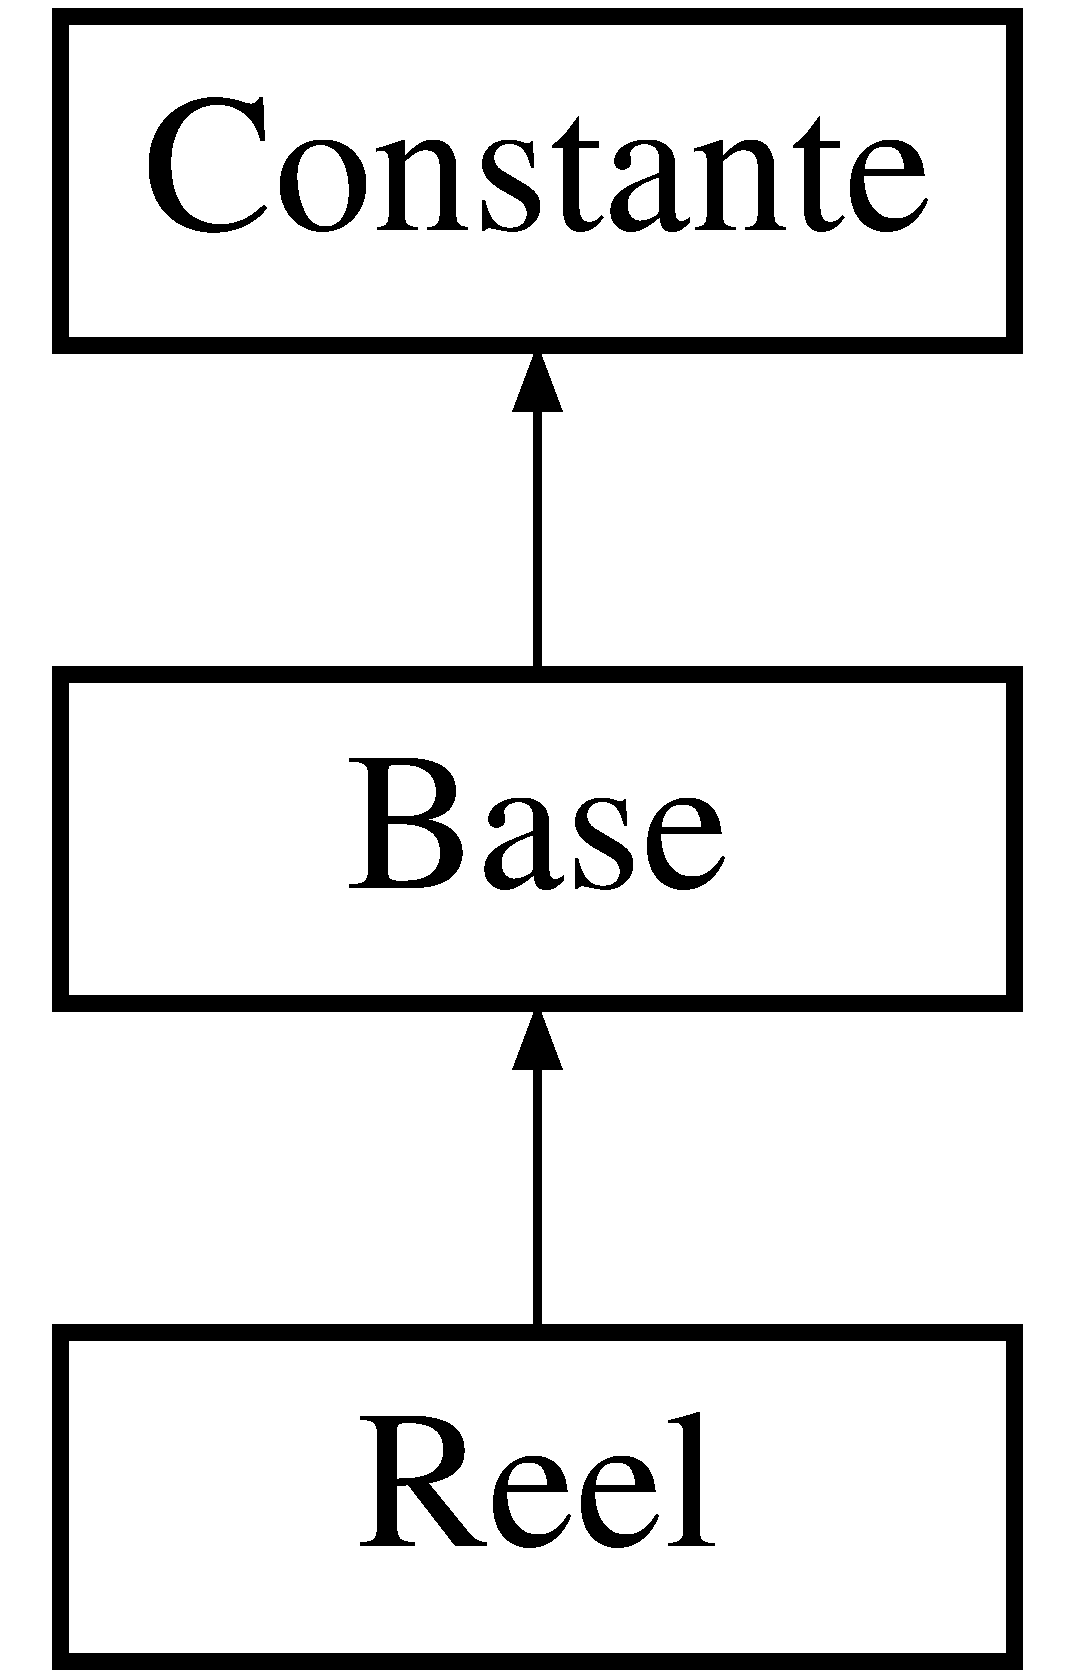
\includegraphics[height=3.000000cm]{class_reel}
\end{center}
\end{figure}
\subsection*{Public Member Functions}
\begin{DoxyCompactItemize}
\item 
\hypertarget{class_reel_ad69ee401f9a73f16abacf65c849fbb7e}{{\bfseries Reel} (double r=0)}\label{class_reel_ad69ee401f9a73f16abacf65c849fbb7e}

\item 
\hypertarget{class_reel_ae3f4716794dd7c64e94ec56accc75dd9}{{\bfseries Reel} (Q\-String s)}\label{class_reel_ae3f4716794dd7c64e94ec56accc75dd9}

\item 
void \hyperlink{class_reel_a52eb23de069729bc2f8b8b2c18e1be7d}{Afficher} (std\-::ostream \&os=std\-::cout) const 
\begin{DoxyCompactList}\small\item\em Fonction virtuelle pour l'affichage, affichant une constante en console. \end{DoxyCompactList}\item 
double \hyperlink{class_reel_a5755a5ed2d9042ad59984967dbddc7f5}{Get\-Val} () const 
\begin{DoxyCompactList}\small\item\em Fonction permettant de récupérer la valeur principale des différentes constantes. \end{DoxyCompactList}\item 
double \hyperlink{class_reel_ab66ca2cb446b1cbc0c3565ff054acc1b}{Get\-Val\-Bis} () const 
\begin{DoxyCompactList}\small\item\em Fonction permettant de récupérer la valeur secondaire des différentes constantes. \end{DoxyCompactList}\item 
const std\-::string \hyperlink{class_reel_ae36b25f3a050292cd6324c0f15dbfb2d}{Get\-Type} () const 
\begin{DoxyCompactList}\small\item\em Fonction permettant de récupérer la valeur du type des différentes constantes. \end{DoxyCompactList}\item 
Q\-String \hyperlink{class_reel_a594333e01d25ecce1335cd25d7cd872e}{Get\-Q\-String} () const 
\begin{DoxyCompactList}\small\item\em Fonction permettant de transformer une \hyperlink{class_constante}{Constante} en Q\-String. \end{DoxyCompactList}\item 
\hypertarget{class_reel_a6a81e5a8d9d1d00e8ec75f4c1e6ca08b}{\hyperlink{class_reel}{Reel} \& {\bfseries operator+} (const \hyperlink{class_reel}{Reel} \&)}\label{class_reel_a6a81e5a8d9d1d00e8ec75f4c1e6ca08b}

\item 
\hypertarget{class_reel_afe46150ca2ed4f283cf7945d78c91365}{\hyperlink{class_reel}{Reel} \& {\bfseries operator+} (const \hyperlink{class_entier}{Entier} \&)}\label{class_reel_afe46150ca2ed4f283cf7945d78c91365}

\item 
\hypertarget{class_reel_a0b4d6f7d33108da029a89fd96a3ca765}{\hyperlink{class_reel}{Reel} \& {\bfseries operator+} (const \hyperlink{class_rationnel}{Rationnel} \&)}\label{class_reel_a0b4d6f7d33108da029a89fd96a3ca765}

\item 
\hypertarget{class_reel_aa7afec89ff0a08582b8609bc77944638}{\hyperlink{class_complexe}{Complexe} \& {\bfseries operator+} (const \hyperlink{class_complexe}{Complexe} \&)}\label{class_reel_aa7afec89ff0a08582b8609bc77944638}

\item 
\hypertarget{class_reel_a3b2d67cac6823259e6d400496f724a59}{\hyperlink{class_expression}{Expression} \& {\bfseries operator+} (\hyperlink{class_expression}{Expression} \&)}\label{class_reel_a3b2d67cac6823259e6d400496f724a59}

\item 
\hypertarget{class_reel_a327dd7c010b30668711287635456181b}{\hyperlink{class_reel}{Reel} \& {\bfseries operator-\/} (const \hyperlink{class_reel}{Reel} \&)}\label{class_reel_a327dd7c010b30668711287635456181b}

\item 
\hypertarget{class_reel_aba49365446030c447113b96d5501d3ed}{\hyperlink{class_reel}{Reel} \& {\bfseries operator-\/} (const \hyperlink{class_entier}{Entier} \&)}\label{class_reel_aba49365446030c447113b96d5501d3ed}

\item 
\hypertarget{class_reel_a565fe37993f7c1c2e5e9ee17e381423d}{\hyperlink{class_reel}{Reel} \& {\bfseries operator-\/} (const \hyperlink{class_rationnel}{Rationnel} \&)}\label{class_reel_a565fe37993f7c1c2e5e9ee17e381423d}

\item 
\hypertarget{class_reel_acdbd1017d5724587741b6796fffad232}{\hyperlink{class_complexe}{Complexe} \& {\bfseries operator-\/} (const \hyperlink{class_complexe}{Complexe} \&)}\label{class_reel_acdbd1017d5724587741b6796fffad232}

\item 
\hypertarget{class_reel_ac4759b066cd89772f5d029891cbddbe7}{\hyperlink{class_expression}{Expression} \& {\bfseries operator-\/} (\hyperlink{class_expression}{Expression} \&)}\label{class_reel_ac4759b066cd89772f5d029891cbddbe7}

\item 
\hypertarget{class_reel_a8f608b10f7e5a9451b1b14b48b8da6c8}{\hyperlink{class_reel}{Reel} \& {\bfseries operator$\ast$} (const \hyperlink{class_reel}{Reel} \&)}\label{class_reel_a8f608b10f7e5a9451b1b14b48b8da6c8}

\item 
\hypertarget{class_reel_a8fcb157bc0d0b7dc57f517cb8d2c50fc}{\hyperlink{class_reel}{Reel} \& {\bfseries operator$\ast$} (const \hyperlink{class_entier}{Entier} \&)}\label{class_reel_a8fcb157bc0d0b7dc57f517cb8d2c50fc}

\item 
\hypertarget{class_reel_aa4e0490eb1266ffa7019f977301a6b25}{\hyperlink{class_reel}{Reel} \& {\bfseries operator$\ast$} (const \hyperlink{class_rationnel}{Rationnel} \&)}\label{class_reel_aa4e0490eb1266ffa7019f977301a6b25}

\item 
\hypertarget{class_reel_ad4265fc39951fe0c29aa6ff53964a60e}{\hyperlink{class_complexe}{Complexe} \& {\bfseries operator$\ast$} (const \hyperlink{class_complexe}{Complexe} \&)}\label{class_reel_ad4265fc39951fe0c29aa6ff53964a60e}

\item 
\hypertarget{class_reel_aac3a12799d8a7d93549eb7dc42beb95d}{\hyperlink{class_expression}{Expression} \& {\bfseries operator$\ast$} (\hyperlink{class_expression}{Expression} \&)}\label{class_reel_aac3a12799d8a7d93549eb7dc42beb95d}

\item 
\hypertarget{class_reel_aeea93660d1c40af04672c7732000e6ff}{\hyperlink{class_reel}{Reel} \& {\bfseries operator/} (const \hyperlink{class_reel}{Reel} \&)}\label{class_reel_aeea93660d1c40af04672c7732000e6ff}

\item 
\hypertarget{class_reel_a25e4ad664b6cf2fe6481f8279e05ab68}{\hyperlink{class_reel}{Reel} \& {\bfseries operator/} (const \hyperlink{class_entier}{Entier} \&)}\label{class_reel_a25e4ad664b6cf2fe6481f8279e05ab68}

\item 
\hypertarget{class_reel_a55fb3390fc076aceccadfba19e5c9ba4}{\hyperlink{class_reel}{Reel} \& {\bfseries operator/} (const \hyperlink{class_rationnel}{Rationnel} \&)}\label{class_reel_a55fb3390fc076aceccadfba19e5c9ba4}

\item 
\hypertarget{class_reel_a130633c75117950f56f319bc15245203}{\hyperlink{class_complexe}{Complexe} \& {\bfseries operator/} (const \hyperlink{class_complexe}{Complexe} \&)}\label{class_reel_a130633c75117950f56f319bc15245203}

\item 
\hypertarget{class_reel_a31869a7f7ededbb5a7f7f28003772a27}{\hyperlink{class_expression}{Expression} \& {\bfseries operator/} (\hyperlink{class_expression}{Expression} \&)}\label{class_reel_a31869a7f7ededbb5a7f7f28003772a27}

\item 
\hypertarget{class_reel_a616d1bee36a89b7b260dfcf20def9b31}{\hyperlink{class_reel}{Reel} \& {\bfseries cos\-Fonction} (std\-::string)}\label{class_reel_a616d1bee36a89b7b260dfcf20def9b31}

\item 
\hypertarget{class_reel_a161e78d47946bf8c378fe3557e48216e}{\hyperlink{class_reel}{Reel} \& {\bfseries sin\-Fonction} (std\-::string)}\label{class_reel_a161e78d47946bf8c378fe3557e48216e}

\item 
\hypertarget{class_reel_aa3255623962ac83582e8f03ec13a46a5}{\hyperlink{class_reel}{Reel} \& {\bfseries tan\-Fonction} (std\-::string)}\label{class_reel_aa3255623962ac83582e8f03ec13a46a5}

\item 
\hypertarget{class_reel_abe5066f774acbc7da0079140fbd9241d}{\hyperlink{class_reel}{Reel} \& {\bfseries cosh\-Fonction} (std\-::string)}\label{class_reel_abe5066f774acbc7da0079140fbd9241d}

\item 
\hypertarget{class_reel_a477be70385a7b3c9fbd7262da79caed0}{\hyperlink{class_reel}{Reel} \& {\bfseries sinh\-Fonction} (std\-::string)}\label{class_reel_a477be70385a7b3c9fbd7262da79caed0}

\item 
\hypertarget{class_reel_a05e059ba72c006f0591018be209e9288}{\hyperlink{class_reel}{Reel} \& {\bfseries tanh\-Fonction} (std\-::string)}\label{class_reel_a05e059ba72c006f0591018be209e9288}

\item 
\hypertarget{class_reel_a46c360be20bcb968e8b885322caf84b9}{\hyperlink{class_reel}{Reel} \& {\bfseries pow\-Fonction} (const \hyperlink{class_entier}{Entier} \&)}\label{class_reel_a46c360be20bcb968e8b885322caf84b9}

\item 
\hypertarget{class_reel_adf1996a2b7dd40325244f9b431eaf814}{\hyperlink{class_reel}{Reel} \& {\bfseries pow\-Fonction} (const \hyperlink{class_reel}{Reel} \&)}\label{class_reel_adf1996a2b7dd40325244f9b431eaf814}

\item 
\hypertarget{class_reel_aac5ad375e6922490462f10e367302117}{\hyperlink{class_reel}{Reel} \& {\bfseries pow\-Fonction} (const \hyperlink{class_rationnel}{Rationnel} \&)}\label{class_reel_aac5ad375e6922490462f10e367302117}

\item 
\hypertarget{class_reel_a446db9edc845242557b6b06ad55e386d}{\hyperlink{class_expression}{Expression} \& {\bfseries pow\-Fonction} (\hyperlink{class_expression}{Expression} \&)}\label{class_reel_a446db9edc845242557b6b06ad55e386d}

\item 
\hypertarget{class_reel_a86cf7d11bb08bf03236bfa90355a921a}{\hyperlink{class_complexe}{Complexe} \& {\bfseries pow\-Fonction} (const \hyperlink{class_complexe}{Complexe} \&)}\label{class_reel_a86cf7d11bb08bf03236bfa90355a921a}

\end{DoxyCompactItemize}


\subsection{Detailed Description}
Classe permettant de représenter le type Réel. 

\subsection{Member Function Documentation}
\hypertarget{class_reel_a52eb23de069729bc2f8b8b2c18e1be7d}{\index{Reel@{Reel}!Afficher@{Afficher}}
\index{Afficher@{Afficher}!Reel@{Reel}}
\subsubsection[{Afficher}]{\setlength{\rightskip}{0pt plus 5cm}void Reel\-::\-Afficher (
\begin{DoxyParamCaption}
\item[{std\-::ostream \&}]{os = {\ttfamily std\-:\-:cout}}
\end{DoxyParamCaption}
) const\hspace{0.3cm}{\ttfamily [inline]}, {\ttfamily [virtual]}}}\label{class_reel_a52eb23de069729bc2f8b8b2c18e1be7d}


Fonction virtuelle pour l'affichage, affichant une constante en console. 


\begin{DoxyParams}{Parameters}
{\em os} & flux d'affichage \\
\hline
\end{DoxyParams}


Implements \hyperlink{class_base_abf809e43ca06c05dcbe3592648a72466}{Base}.

\hypertarget{class_reel_a594333e01d25ecce1335cd25d7cd872e}{\index{Reel@{Reel}!Get\-Q\-String@{Get\-Q\-String}}
\index{Get\-Q\-String@{Get\-Q\-String}!Reel@{Reel}}
\subsubsection[{Get\-Q\-String}]{\setlength{\rightskip}{0pt plus 5cm}Q\-String Reel\-::\-Get\-Q\-String (
\begin{DoxyParamCaption}
{}
\end{DoxyParamCaption}
) const\hspace{0.3cm}{\ttfamily [inline]}, {\ttfamily [virtual]}}}\label{class_reel_a594333e01d25ecce1335cd25d7cd872e}


Fonction permettant de transformer une \hyperlink{class_constante}{Constante} en Q\-String. 

\begin{DoxyReturn}{Returns}
Q\-String. 
\end{DoxyReturn}


Implements \hyperlink{class_constante_a7c3edb9082492c95eb319da3d42bb7a4}{Constante}.

\hypertarget{class_reel_ae36b25f3a050292cd6324c0f15dbfb2d}{\index{Reel@{Reel}!Get\-Type@{Get\-Type}}
\index{Get\-Type@{Get\-Type}!Reel@{Reel}}
\subsubsection[{Get\-Type}]{\setlength{\rightskip}{0pt plus 5cm}const std\-::string Reel\-::\-Get\-Type (
\begin{DoxyParamCaption}
{}
\end{DoxyParamCaption}
) const\hspace{0.3cm}{\ttfamily [inline]}, {\ttfamily [virtual]}}}\label{class_reel_ae36b25f3a050292cd6324c0f15dbfb2d}


Fonction permettant de récupérer la valeur du type des différentes constantes. 

\begin{DoxyReturn}{Returns}
String. 
\end{DoxyReturn}


Implements \hyperlink{class_constante_a2f716a85b9b519b7bbf8ed8d997f66d3}{Constante}.

\hypertarget{class_reel_a5755a5ed2d9042ad59984967dbddc7f5}{\index{Reel@{Reel}!Get\-Val@{Get\-Val}}
\index{Get\-Val@{Get\-Val}!Reel@{Reel}}
\subsubsection[{Get\-Val}]{\setlength{\rightskip}{0pt plus 5cm}double Reel\-::\-Get\-Val (
\begin{DoxyParamCaption}
{}
\end{DoxyParamCaption}
) const\hspace{0.3cm}{\ttfamily [inline]}, {\ttfamily [virtual]}}}\label{class_reel_a5755a5ed2d9042ad59984967dbddc7f5}


Fonction permettant de récupérer la valeur principale des différentes constantes. 

\begin{DoxyReturn}{Returns}
Double. 
\end{DoxyReturn}


Implements \hyperlink{class_constante_af88eb444ed659cc6bb2f9571326a9eb1}{Constante}.

\hypertarget{class_reel_ab66ca2cb446b1cbc0c3565ff054acc1b}{\index{Reel@{Reel}!Get\-Val\-Bis@{Get\-Val\-Bis}}
\index{Get\-Val\-Bis@{Get\-Val\-Bis}!Reel@{Reel}}
\subsubsection[{Get\-Val\-Bis}]{\setlength{\rightskip}{0pt plus 5cm}double Reel\-::\-Get\-Val\-Bis (
\begin{DoxyParamCaption}
{}
\end{DoxyParamCaption}
) const\hspace{0.3cm}{\ttfamily [inline]}, {\ttfamily [virtual]}}}\label{class_reel_ab66ca2cb446b1cbc0c3565ff054acc1b}


Fonction permettant de récupérer la valeur secondaire des différentes constantes. 

\begin{DoxyReturn}{Returns}
Double. 
\end{DoxyReturn}


Implements \hyperlink{class_constante_aa0602d62c04f28f7bda68723f5dbc48b}{Constante}.



The documentation for this class was generated from the following files\-:\begin{DoxyCompactItemize}
\item 
\hyperlink{constante_8h}{constante.\-h}\item 
constante\-Op\-Div.\-cpp\item 
constante\-Op\-Moins.\-cpp\item 
constante\-Op\-Mult.\-cpp\item 
constante\-Op\-Plus.\-cpp\item 
constante\-Op\-Pow.\-cpp\item 
operateurs\-Unaires.\-cpp\end{DoxyCompactItemize}

\hypertarget{class_ui___main_window}{\section{Ui\-\_\-\-Main\-Window Class Reference}
\label{class_ui___main_window}\index{Ui\-\_\-\-Main\-Window@{Ui\-\_\-\-Main\-Window}}
}
Inheritance diagram for Ui\-\_\-\-Main\-Window\-:\begin{figure}[H]
\begin{center}
\leavevmode
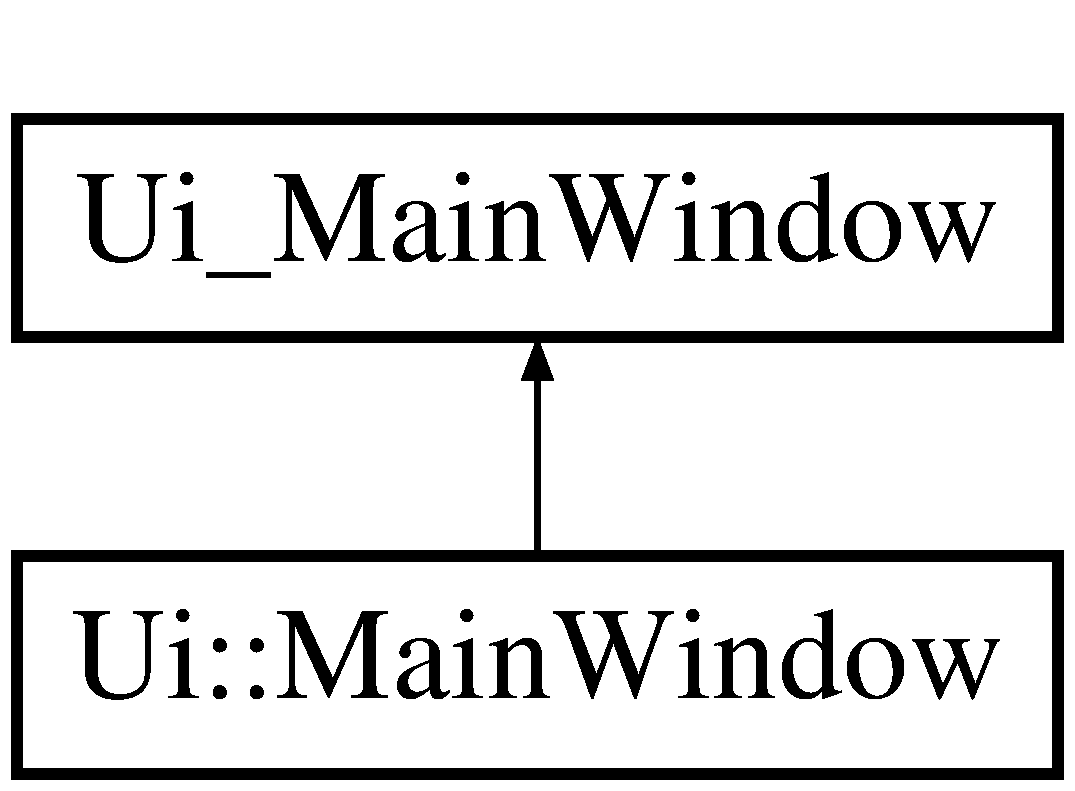
\includegraphics[height=2.000000cm]{class_ui___main_window}
\end{center}
\end{figure}
\subsection*{Public Member Functions}
\begin{DoxyCompactItemize}
\item 
\hypertarget{class_ui___main_window_acf4a0872c4c77d8f43a2ec66ed849b58}{void {\bfseries setup\-Ui} (Q\-Main\-Window $\ast$\hyperlink{class_main_window}{Main\-Window})}\label{class_ui___main_window_acf4a0872c4c77d8f43a2ec66ed849b58}

\item 
\hypertarget{class_ui___main_window_a097dd160c3534a204904cb374412c618}{void {\bfseries retranslate\-Ui} (Q\-Main\-Window $\ast$\hyperlink{class_main_window}{Main\-Window})}\label{class_ui___main_window_a097dd160c3534a204904cb374412c618}

\end{DoxyCompactItemize}
\subsection*{Public Attributes}
\begin{DoxyCompactItemize}
\item 
\hypertarget{class_ui___main_window_a188c243f36a2dbc10e4e2a0ad94273b1}{Q\-Action $\ast$ {\bfseries action\-Quit}}\label{class_ui___main_window_a188c243f36a2dbc10e4e2a0ad94273b1}

\item 
\hypertarget{class_ui___main_window_abdf2b43167c2cd0d3405f90b8c30e934}{Q\-Action $\ast$ {\bfseries action\-About}}\label{class_ui___main_window_abdf2b43167c2cd0d3405f90b8c30e934}

\item 
\hypertarget{class_ui___main_window_a601a1ba9e9445f0ca1b26dfa67a78703}{Q\-Action $\ast$ {\bfseries action\-Retablir}}\label{class_ui___main_window_a601a1ba9e9445f0ca1b26dfa67a78703}

\item 
\hypertarget{class_ui___main_window_a664bb393ac59ffa411d7e9b3afff406f}{Q\-Action $\ast$ {\bfseries action\-Annuler}}\label{class_ui___main_window_a664bb393ac59ffa411d7e9b3afff406f}

\item 
\hypertarget{class_ui___main_window_a63f9fe57d2cb76fe2d4180a5ea63c554}{Q\-Action $\ast$ {\bfseries action\-Mode\-\_\-\-Complexe}}\label{class_ui___main_window_a63f9fe57d2cb76fe2d4180a5ea63c554}

\item 
\hypertarget{class_ui___main_window_ac69ed0b5ddad47458152a0ccea579e99}{Q\-Action $\ast$ {\bfseries action\-Clavier}}\label{class_ui___main_window_ac69ed0b5ddad47458152a0ccea579e99}

\item 
\hypertarget{class_ui___main_window_ab043cd3ce5b589be82c36a391a448ed8}{Q\-Action $\ast$ {\bfseries action\-Entier}}\label{class_ui___main_window_ab043cd3ce5b589be82c36a391a448ed8}

\item 
\hypertarget{class_ui___main_window_ad0dc959d5365caf61a470875ac938c2b}{Q\-Action $\ast$ {\bfseries action\-Reel}}\label{class_ui___main_window_ad0dc959d5365caf61a470875ac938c2b}

\item 
\hypertarget{class_ui___main_window_a1a6107ceba6147d13f11b75b5128dc7d}{Q\-Action $\ast$ {\bfseries action\-Rationnel}}\label{class_ui___main_window_a1a6107ceba6147d13f11b75b5128dc7d}

\item 
\hypertarget{class_ui___main_window_ab72db212996c87f8c93c52e66ab260b6}{Q\-Action $\ast$ {\bfseries action\-Degres}}\label{class_ui___main_window_ab72db212996c87f8c93c52e66ab260b6}

\item 
\hypertarget{class_ui___main_window_ad79f4a35f50b1e68f19181e9198bc016}{Q\-Action $\ast$ {\bfseries action\-Radians}}\label{class_ui___main_window_ad79f4a35f50b1e68f19181e9198bc016}

\item 
\hypertarget{class_ui___main_window_aa857263056fc43ce72b834e818354efd}{Q\-Action $\ast$ {\bfseries action2}}\label{class_ui___main_window_aa857263056fc43ce72b834e818354efd}

\item 
\hypertarget{class_ui___main_window_a92d77f31e41cf2fbc51b63cd55f658ee}{Q\-Action $\ast$ {\bfseries action1}}\label{class_ui___main_window_a92d77f31e41cf2fbc51b63cd55f658ee}

\item 
\hypertarget{class_ui___main_window_a30075506c2116c3ed4ff25e07ae75f81}{Q\-Widget $\ast$ {\bfseries central\-Widget}}\label{class_ui___main_window_a30075506c2116c3ed4ff25e07ae75f81}

\item 
\hypertarget{class_ui___main_window_a9271976c4376de565bfe96c296f4db1e}{Q\-Widget $\ast$ {\bfseries horizontal\-Layout\-Widget}}\label{class_ui___main_window_a9271976c4376de565bfe96c296f4db1e}

\item 
\hypertarget{class_ui___main_window_acd6fdc9ebacc4b25b834162380d75ce8}{Q\-H\-Box\-Layout $\ast$ {\bfseries horizontal\-Layout}}\label{class_ui___main_window_acd6fdc9ebacc4b25b834162380d75ce8}

\item 
\hypertarget{class_ui___main_window_ae236fa9b0d651ccf713e7a81e35497fe}{Q\-V\-Box\-Layout $\ast$ {\bfseries clavier\-Layout}}\label{class_ui___main_window_ae236fa9b0d651ccf713e7a81e35497fe}

\item 
\hypertarget{class_ui___main_window_a6b2a0c5f7e8ff2a87134908dd770d2d2}{Q\-Grid\-Layout $\ast$ {\bfseries grid\-Layout\-\_\-2}}\label{class_ui___main_window_a6b2a0c5f7e8ff2a87134908dd770d2d2}

\item 
\hypertarget{class_ui___main_window_ad722b8ecf971b4db2026e8ff6431762f}{Q\-Push\-Button $\ast$ {\bfseries un}}\label{class_ui___main_window_ad722b8ecf971b4db2026e8ff6431762f}

\item 
\hypertarget{class_ui___main_window_a55c4428f1aa4f70d81c0682428d56937}{Q\-Push\-Button $\ast$ {\bfseries trois}}\label{class_ui___main_window_a55c4428f1aa4f70d81c0682428d56937}

\item 
\hypertarget{class_ui___main_window_a144c019ae08032b82b2ab95fcb608444}{Q\-Push\-Button $\ast$ {\bfseries deux}}\label{class_ui___main_window_a144c019ae08032b82b2ab95fcb608444}

\item 
\hypertarget{class_ui___main_window_a9748c418a105b8c49076fe9bc8577d28}{Q\-Push\-Button $\ast$ {\bfseries quatre}}\label{class_ui___main_window_a9748c418a105b8c49076fe9bc8577d28}

\item 
\hypertarget{class_ui___main_window_a26b51feb3661651d222c1e0360610a98}{Q\-Push\-Button $\ast$ {\bfseries sept}}\label{class_ui___main_window_a26b51feb3661651d222c1e0360610a98}

\item 
\hypertarget{class_ui___main_window_a8cdd950853ab23cb9563920a4f8e85c5}{Q\-Push\-Button $\ast$ {\bfseries cinq}}\label{class_ui___main_window_a8cdd950853ab23cb9563920a4f8e85c5}

\item 
\hypertarget{class_ui___main_window_a6d9c471a35a1d7a58d057f841c57cb93}{Q\-Push\-Button $\ast$ {\bfseries huit}}\label{class_ui___main_window_a6d9c471a35a1d7a58d057f841c57cb93}

\item 
\hypertarget{class_ui___main_window_a051d07272ec800040b2a9b0bc6031047}{Q\-Push\-Button $\ast$ {\bfseries neuf}}\label{class_ui___main_window_a051d07272ec800040b2a9b0bc6031047}

\item 
\hypertarget{class_ui___main_window_a14af2869e1247a2ab4ca797b3930e30f}{Q\-Push\-Button $\ast$ {\bfseries six}}\label{class_ui___main_window_a14af2869e1247a2ab4ca797b3930e30f}

\item 
\hypertarget{class_ui___main_window_acce7707852833af1c8c231eddd732e30}{Q\-Push\-Button $\ast$ {\bfseries cmplx}}\label{class_ui___main_window_acce7707852833af1c8c231eddd732e30}

\item 
\hypertarget{class_ui___main_window_af8100100d8104ac094e3b7a2999b5152}{Q\-Push\-Button $\ast$ {\bfseries expr}}\label{class_ui___main_window_af8100100d8104ac094e3b7a2999b5152}

\item 
\hypertarget{class_ui___main_window_ad33006fc17936efa48bc71381c25a82b}{Q\-Push\-Button $\ast$ {\bfseries coma}}\label{class_ui___main_window_ad33006fc17936efa48bc71381c25a82b}

\item 
\hypertarget{class_ui___main_window_a147d7b0bc267d1797b13690f66875694}{Q\-Push\-Button $\ast$ {\bfseries del}}\label{class_ui___main_window_a147d7b0bc267d1797b13690f66875694}

\item 
\hypertarget{class_ui___main_window_a4a501f5ffc49af12d0c2ed22438daeef}{Q\-Push\-Button $\ast$ {\bfseries zero}}\label{class_ui___main_window_a4a501f5ffc49af12d0c2ed22438daeef}

\item 
\hypertarget{class_ui___main_window_a4ddf7c4ab13f19e86300500b321b003c}{Q\-Push\-Button $\ast$ {\bfseries entrer}}\label{class_ui___main_window_a4ddf7c4ab13f19e86300500b321b003c}

\item 
\hypertarget{class_ui___main_window_aeb5ba85c74a147d349e190d4c5379423}{Q\-Push\-Button $\ast$ {\bfseries x\-Egal}}\label{class_ui___main_window_aeb5ba85c74a147d349e190d4c5379423}

\item 
\hypertarget{class_ui___main_window_af4bbe1414fac62cfb02b107382150f3d}{Q\-Push\-Button $\ast$ {\bfseries x}}\label{class_ui___main_window_af4bbe1414fac62cfb02b107382150f3d}

\item 
\hypertarget{class_ui___main_window_a53b2892737afd6147b05470d90c1c25d}{Q\-Spacer\-Item $\ast$ {\bfseries espace1}}\label{class_ui___main_window_a53b2892737afd6147b05470d90c1c25d}

\item 
\hypertarget{class_ui___main_window_a0800cb2041227f892d21aeb968fd93db}{Q\-Label $\ast$ {\bfseries op\-Binaires}}\label{class_ui___main_window_a0800cb2041227f892d21aeb968fd93db}

\item 
\hypertarget{class_ui___main_window_a525ed3c5fe0784ac502ee222fba4e205}{Q\-Grid\-Layout $\ast$ {\bfseries grid\-Layout}}\label{class_ui___main_window_a525ed3c5fe0784ac502ee222fba4e205}

\item 
\hypertarget{class_ui___main_window_ab529ca58e125e2f64435f541216421a3}{Q\-Push\-Button $\ast$ {\bfseries div}}\label{class_ui___main_window_ab529ca58e125e2f64435f541216421a3}

\item 
\hypertarget{class_ui___main_window_a186af8eccf20a88509bab0284e8b43ba}{Q\-Push\-Button $\ast$ {\bfseries plus}}\label{class_ui___main_window_a186af8eccf20a88509bab0284e8b43ba}

\item 
\hypertarget{class_ui___main_window_a1e5405d49cd9c0dff806441988765dc5}{Q\-Push\-Button $\ast$ {\bfseries moins}}\label{class_ui___main_window_a1e5405d49cd9c0dff806441988765dc5}

\item 
\hypertarget{class_ui___main_window_a816519bcd5dbd62552ec153ebb1c0d86}{Q\-Push\-Button $\ast$ {\bfseries multi}}\label{class_ui___main_window_a816519bcd5dbd62552ec153ebb1c0d86}

\item 
\hypertarget{class_ui___main_window_a865b77e9ebfbfcae23894310183052c2}{Q\-Push\-Button $\ast$ {\bfseries pow}}\label{class_ui___main_window_a865b77e9ebfbfcae23894310183052c2}

\item 
\hypertarget{class_ui___main_window_a160e0e73eef61779e82549a085ac7c2b}{Q\-Push\-Button $\ast$ {\bfseries mod}}\label{class_ui___main_window_a160e0e73eef61779e82549a085ac7c2b}

\item 
\hypertarget{class_ui___main_window_ac72755bbdeb9867dfa66c194c7a556d2}{Q\-Spacer\-Item $\ast$ {\bfseries espace2}}\label{class_ui___main_window_ac72755bbdeb9867dfa66c194c7a556d2}

\item 
\hypertarget{class_ui___main_window_aeb97af58c0eef49eef9307d08ed59346}{Q\-Label $\ast$ {\bfseries op\-Unaires}}\label{class_ui___main_window_aeb97af58c0eef49eef9307d08ed59346}

\item 
\hypertarget{class_ui___main_window_af42ea7d4c2e893181caad21e28166932}{Q\-Grid\-Layout $\ast$ {\bfseries grid\-Layout\-\_\-3}}\label{class_ui___main_window_af42ea7d4c2e893181caad21e28166932}

\item 
\hypertarget{class_ui___main_window_aa0dce255726f689c6c0934a3d244b527}{Q\-Push\-Button $\ast$ {\bfseries cosh}}\label{class_ui___main_window_aa0dce255726f689c6c0934a3d244b527}

\item 
\hypertarget{class_ui___main_window_a30da6abc5c5022307d700912a9f0e05c}{Q\-Push\-Button $\ast$ {\bfseries sqrt}}\label{class_ui___main_window_a30da6abc5c5022307d700912a9f0e05c}

\item 
\hypertarget{class_ui___main_window_abbbbfd1b1d4213c977d130f1075fd5c3}{Q\-Push\-Button $\ast$ {\bfseries sin}}\label{class_ui___main_window_abbbbfd1b1d4213c977d130f1075fd5c3}

\item 
\hypertarget{class_ui___main_window_afbe7546443ae7cb8ecd6b44daaa118cd}{Q\-Push\-Button $\ast$ {\bfseries sqr}}\label{class_ui___main_window_afbe7546443ae7cb8ecd6b44daaa118cd}

\item 
\hypertarget{class_ui___main_window_aabb62a971c22cd9da15be1454401cac5}{Q\-Push\-Button $\ast$ {\bfseries tanh}}\label{class_ui___main_window_aabb62a971c22cd9da15be1454401cac5}

\item 
\hypertarget{class_ui___main_window_afd3c06256497bbb5b47c964c7effe236}{Q\-Push\-Button $\ast$ {\bfseries log}}\label{class_ui___main_window_afd3c06256497bbb5b47c964c7effe236}

\item 
\hypertarget{class_ui___main_window_af7e7fbd7b5b9271ed1886de0e5ac6557}{Q\-Push\-Button $\ast$ {\bfseries sinh}}\label{class_ui___main_window_af7e7fbd7b5b9271ed1886de0e5ac6557}

\item 
\hypertarget{class_ui___main_window_a1b22341166bce0619d82b4f332795984}{Q\-Push\-Button $\ast$ {\bfseries inv}}\label{class_ui___main_window_a1b22341166bce0619d82b4f332795984}

\item 
\hypertarget{class_ui___main_window_a1bc6bc9c9775737a720869fafba88562}{Q\-Push\-Button $\ast$ {\bfseries ln}}\label{class_ui___main_window_a1bc6bc9c9775737a720869fafba88562}

\item 
\hypertarget{class_ui___main_window_ace2fc9efb31fe2d32ef7c1ee3c3f00b9}{Q\-Push\-Button $\ast$ {\bfseries tan}}\label{class_ui___main_window_ace2fc9efb31fe2d32ef7c1ee3c3f00b9}

\item 
\hypertarget{class_ui___main_window_aa3c6f207926229866f26184d1200ac7f}{Q\-Push\-Button $\ast$ {\bfseries cos}}\label{class_ui___main_window_aa3c6f207926229866f26184d1200ac7f}

\item 
\hypertarget{class_ui___main_window_adaa8072bddbae3ddefe06e9e3a133790}{Q\-Push\-Button $\ast$ {\bfseries cube}}\label{class_ui___main_window_adaa8072bddbae3ddefe06e9e3a133790}

\item 
\hypertarget{class_ui___main_window_ab9e5d07669e9d976a6f36079cc2c05b7}{Q\-Push\-Button $\ast$ {\bfseries fact}}\label{class_ui___main_window_ab9e5d07669e9d976a6f36079cc2c05b7}

\item 
\hypertarget{class_ui___main_window_a310a072a24f117b239d80ca5e16d091e}{Q\-Push\-Button $\ast$ {\bfseries sign}}\label{class_ui___main_window_a310a072a24f117b239d80ca5e16d091e}

\item 
\hypertarget{class_ui___main_window_a4a5c262f25072172b908e0addd2b4a68}{Q\-Push\-Button $\ast$ {\bfseries eval}}\label{class_ui___main_window_a4a5c262f25072172b908e0addd2b4a68}

\item 
\hypertarget{class_ui___main_window_a36ab42c08ae5c0af03f35bad111b849e}{Q\-Spacer\-Item $\ast$ {\bfseries espace3}}\label{class_ui___main_window_a36ab42c08ae5c0af03f35bad111b849e}

\item 
\hypertarget{class_ui___main_window_a877f1866923f76b6cee8fc6fd1b47149}{Q\-Label $\ast$ {\bfseries op\-Pile}}\label{class_ui___main_window_a877f1866923f76b6cee8fc6fd1b47149}

\item 
\hypertarget{class_ui___main_window_a8ee86315639f324b17708efc7dbe8b19}{Q\-Grid\-Layout $\ast$ {\bfseries grid\-Layout\-\_\-4}}\label{class_ui___main_window_a8ee86315639f324b17708efc7dbe8b19}

\item 
\hypertarget{class_ui___main_window_a06447b27a6b617797f1935c0da8b4fca}{Q\-Push\-Button $\ast$ {\bfseries dup}}\label{class_ui___main_window_a06447b27a6b617797f1935c0da8b4fca}

\item 
\hypertarget{class_ui___main_window_af99377dc93c5c55a8fcb556539ee0b14}{Q\-Push\-Button $\ast$ {\bfseries sum}}\label{class_ui___main_window_af99377dc93c5c55a8fcb556539ee0b14}

\item 
\hypertarget{class_ui___main_window_a69c4ef9eebd49f9bf048e056f8b3ee84}{Q\-Push\-Button $\ast$ {\bfseries swap}}\label{class_ui___main_window_a69c4ef9eebd49f9bf048e056f8b3ee84}

\item 
\hypertarget{class_ui___main_window_a5fb7e7ae0ff9593f591858fb648053a3}{Q\-Push\-Button $\ast$ {\bfseries mean}}\label{class_ui___main_window_a5fb7e7ae0ff9593f591858fb648053a3}

\item 
\hypertarget{class_ui___main_window_a77911a9fd66fb7b7ccb5d6194e960d33}{Q\-Push\-Button $\ast$ {\bfseries clear}}\label{class_ui___main_window_a77911a9fd66fb7b7ccb5d6194e960d33}

\item 
\hypertarget{class_ui___main_window_a93cc1019ad407d063ab0c95714bbdbd2}{Q\-Push\-Button $\ast$ {\bfseries drop}}\label{class_ui___main_window_a93cc1019ad407d063ab0c95714bbdbd2}

\item 
\hypertarget{class_ui___main_window_a7871ea8c4b6c595d7ccd53960b344719}{Q\-Spacer\-Item $\ast$ {\bfseries horizontal\-Spacer}}\label{class_ui___main_window_a7871ea8c4b6c595d7ccd53960b344719}

\item 
\hypertarget{class_ui___main_window_a72e8a5a26cf0578c234118acc6ca28ab}{Q\-V\-Box\-Layout $\ast$ {\bfseries ecrans}}\label{class_ui___main_window_a72e8a5a26cf0578c234118acc6ca28ab}

\item 
\hypertarget{class_ui___main_window_a576c4f161d89da516666f039f260cdca}{Q\-Line\-Edit $\ast$ {\bfseries champ\-Ecr}}\label{class_ui___main_window_a576c4f161d89da516666f039f260cdca}

\item 
\hypertarget{class_ui___main_window_a8384329c3663ff274e926a12024aab52}{Q\-Spacer\-Item $\ast$ {\bfseries vertical\-Spacer}}\label{class_ui___main_window_a8384329c3663ff274e926a12024aab52}

\item 
\hypertarget{class_ui___main_window_a5d861666785153778e31351e64e2f68d}{Q\-Text\-Edit $\ast$ {\bfseries champ\-Aff}}\label{class_ui___main_window_a5d861666785153778e31351e64e2f68d}

\item 
\hypertarget{class_ui___main_window_adc1f5fdd97fb3729999c56902d0fa591}{Q\-Spacer\-Item $\ast$ {\bfseries vertical\-Spacer\-\_\-2}}\label{class_ui___main_window_adc1f5fdd97fb3729999c56902d0fa591}

\item 
\hypertarget{class_ui___main_window_a03ce63974cc69b067c91bbf285cceca8}{Q\-H\-Box\-Layout $\ast$ {\bfseries horizontal\-Layout\-\_\-3}}\label{class_ui___main_window_a03ce63974cc69b067c91bbf285cceca8}

\item 
\hypertarget{class_ui___main_window_a2e2516d755e4dd53fc905dabddf2738a}{Q\-Label $\ast$ {\bfseries label\-\_\-2}}\label{class_ui___main_window_a2e2516d755e4dd53fc905dabddf2738a}

\item 
\hypertarget{class_ui___main_window_a5ed8c322ed5b78af28d9810275a6b93c}{Q\-Line\-Edit $\ast$ {\bfseries champ\-Nb\-Aff}}\label{class_ui___main_window_a5ed8c322ed5b78af28d9810275a6b93c}

\item 
\hypertarget{class_ui___main_window_a21419cdc67fc93bad238bfccb1bdec9f}{Q\-Line\-Edit $\ast$ {\bfseries champ\-Err}}\label{class_ui___main_window_a21419cdc67fc93bad238bfccb1bdec9f}

\item 
\hypertarget{class_ui___main_window_a2be1c24ec9adfca18e1dcc951931457f}{Q\-Menu\-Bar $\ast$ {\bfseries menu\-Bar}}\label{class_ui___main_window_a2be1c24ec9adfca18e1dcc951931457f}

\item 
\hypertarget{class_ui___main_window_a6d7bbbef44e207ee15e5a623171033a2}{Q\-Menu $\ast$ {\bfseries menu\-Menu}}\label{class_ui___main_window_a6d7bbbef44e207ee15e5a623171033a2}

\item 
\hypertarget{class_ui___main_window_a620838edd0b215733f1ab0f0ec8af026}{Q\-Menu $\ast$ {\bfseries menu\-Param}}\label{class_ui___main_window_a620838edd0b215733f1ab0f0ec8af026}

\item 
\hypertarget{class_ui___main_window_a24c329f45c723c83d4fddebf105b3fc6}{Q\-Menu $\ast$ {\bfseries menu\-Type\-\_\-de\-\_\-\-Constante}}\label{class_ui___main_window_a24c329f45c723c83d4fddebf105b3fc6}

\item 
\hypertarget{class_ui___main_window_a345a4ec92e6309977909efe6600b45c1}{Q\-Menu $\ast$ {\bfseries menu\-Angle}}\label{class_ui___main_window_a345a4ec92e6309977909efe6600b45c1}

\item 
\hypertarget{class_ui___main_window_a90b7838eb41442b6dab6593fe61bbb58}{Q\-Menu $\ast$ {\bfseries menu\-Affichage}}\label{class_ui___main_window_a90b7838eb41442b6dab6593fe61bbb58}

\item 
\hypertarget{class_ui___main_window_a5172877001c8c7b4e0f6de50421867d1}{Q\-Tool\-Bar $\ast$ {\bfseries main\-Tool\-Bar}}\label{class_ui___main_window_a5172877001c8c7b4e0f6de50421867d1}

\item 
\hypertarget{class_ui___main_window_a50fa481337604bcc8bf68de18ab16ecd}{Q\-Status\-Bar $\ast$ {\bfseries status\-Bar}}\label{class_ui___main_window_a50fa481337604bcc8bf68de18ab16ecd}

\end{DoxyCompactItemize}


The documentation for this class was generated from the following file\-:\begin{DoxyCompactItemize}
\item 
ui\-\_\-mainwindow.\-h\end{DoxyCompactItemize}

\chapter{File Documentation}
\hypertarget{constante_8h}{\section{constante.\-h File Reference}
\label{constante_8h}\index{constante.\-h@{constante.\-h}}
}


Déclaration de la classe \hyperlink{class_constante}{Constante} et de ses classes filles.  


{\ttfamily \#include $<$iostream$>$}\\*
{\ttfamily \#include $<$string$>$}\\*
{\ttfamily \#include $<$Q\-String$>$}\\*
{\ttfamily \#include $<$deque$>$}\\*
{\ttfamily \#include \char`\"{}exception\-Calculatrice.\-h\char`\"{}}\\*
\subsection*{Classes}
\begin{DoxyCompactItemize}
\item 
class \hyperlink{class_constante}{Constante}
\begin{DoxyCompactList}\small\item\em Classe mère de toutes les valeurs empilées dans la pile de stockage. \end{DoxyCompactList}\item 
class \hyperlink{class_expression}{Expression}
\begin{DoxyCompactList}\small\item\em Classe permettant de gérer le type expression pouvant être évaluer à tout moment. \end{DoxyCompactList}\item 
class \hyperlink{class_base}{Base}
\begin{DoxyCompactList}\small\item\em Classe englobant les types \hyperlink{class_rationnel}{Rationnel}, Réel et \hyperlink{class_entier}{Entier}. Elle compose la classe \hyperlink{class_complexe}{Complexe}. \end{DoxyCompactList}\item 
class \hyperlink{class_complexe}{Complexe}
\begin{DoxyCompactList}\small\item\em Classe permettant de représenter le type \hyperlink{class_complexe}{Complexe}. Chacune de ses parties (Réelle \& Imaginaire) est une \hyperlink{class_base}{Base}. \end{DoxyCompactList}\item 
class \hyperlink{class_reel}{Reel}
\begin{DoxyCompactList}\small\item\em Classe permettant de représenter le type Réel. \end{DoxyCompactList}\item 
class \hyperlink{class_rationnel}{Rationnel}
\begin{DoxyCompactList}\small\item\em Classe permettant de représenter le type \hyperlink{class_rationnel}{Rationnel}. \end{DoxyCompactList}\item 
class \hyperlink{class_entier}{Entier}
\begin{DoxyCompactList}\small\item\em Classe permettant de représenter le type \hyperlink{class_entier}{Entier}. \end{DoxyCompactList}\end{DoxyCompactItemize}


\subsection{Detailed Description}
Déclaration de la classe \hyperlink{class_constante}{Constante} et de ses classes filles. \begin{DoxyAuthor}{Author}
Agathe Oddon et Jean-\/\-Michel Tozzini 
\end{DoxyAuthor}
\begin{DoxyDate}{Date}
10/06/2012 
\end{DoxyDate}
\begin{DoxyVersion}{Version}
1 
\end{DoxyVersion}

\hypertarget{exception_calculatrice_8h}{\section{exception\-Calculatrice.\-h File Reference}
\label{exception_calculatrice_8h}\index{exception\-Calculatrice.\-h@{exception\-Calculatrice.\-h}}
}


Déclaration de la classe \hyperlink{class_exception_calculatrice}{Exception\-Calculatrice} pour la gestion des erreurs.  


{\ttfamily \#include $<$Q\-String$>$}\\*
\subsection*{Classes}
\begin{DoxyCompactItemize}
\item 
class \hyperlink{class_exception_calculatrice}{Exception\-Calculatrice}
\begin{DoxyCompactList}\small\item\em Classe permettant de gérer les exceptions de la calculatrice. \end{DoxyCompactList}\end{DoxyCompactItemize}


\subsection{Detailed Description}
Déclaration de la classe \hyperlink{class_exception_calculatrice}{Exception\-Calculatrice} pour la gestion des erreurs. 
\hypertarget{fonctions_annexe_8h}{\section{fonctions\-Annexe.\-h File Reference}
\label{fonctions_annexe_8h}\index{fonctions\-Annexe.\-h@{fonctions\-Annexe.\-h}}
}


Fonctions annexes de la calculatrice.  


{\ttfamily \#include \char`\"{}mainwindow.\-h\char`\"{}}\\*
\subsection*{Functions}
\begin{DoxyCompactItemize}
\item 
\hypertarget{fonctions_annexe_8h_a07963291b6fb7c408ade66928d778312}{\hyperlink{class_reel}{Reel} $\ast$ \hyperlink{fonctions_annexe_8h_a07963291b6fb7c408ade66928d778312}{To\-Reel} (Q\-String \&s)}\label{fonctions_annexe_8h_a07963291b6fb7c408ade66928d778312}

\begin{DoxyCompactList}\small\item\em Fonction permettant de transformer une chaine de caractères en Réel. \end{DoxyCompactList}\item 
\hypertarget{fonctions_annexe_8h_af0d05a6fc5e62857788fbb75338c263d}{\hyperlink{class_rationnel}{Rationnel} $\ast$ \hyperlink{fonctions_annexe_8h_af0d05a6fc5e62857788fbb75338c263d}{To\-Rationnel} (Q\-String \&s)}\label{fonctions_annexe_8h_af0d05a6fc5e62857788fbb75338c263d}

\begin{DoxyCompactList}\small\item\em Fonction permettant de transformer une chaine de caractères en \hyperlink{class_rationnel}{Rationnel}. \end{DoxyCompactList}\item 
\hypertarget{fonctions_annexe_8h_afa311af6a885cc03175db5469ed9af77}{\hyperlink{class_complexe}{Complexe} $\ast$ \hyperlink{fonctions_annexe_8h_afa311af6a885cc03175db5469ed9af77}{To\-Complexe} (Q\-String \&s)}\label{fonctions_annexe_8h_afa311af6a885cc03175db5469ed9af77}

\begin{DoxyCompactList}\small\item\em Fonction permettant de transformer une chaine de caractères en \hyperlink{class_complexe}{Complexe}. \end{DoxyCompactList}\item 
int \hyperlink{fonctions_annexe_8h_a3f795b7c84579c18c10d07a9202de3d5}{P\-G\-C\-D} (int, int)
\begin{DoxyCompactList}\small\item\em Fonction permettant de calculer le P\-G\-C\-D de deux int. \end{DoxyCompactList}\item 
int \hyperlink{fonctions_annexe_8h_a2fd8fce0aad78a0f5a80a682ed4a63eb}{Factorielle} (int)
\begin{DoxyCompactList}\small\item\em Fonction permettant de calculer la factorielle d'un int. \end{DoxyCompactList}\end{DoxyCompactItemize}


\subsection{Detailed Description}
Fonctions annexes de la calculatrice. 

\subsection{Function Documentation}
\hypertarget{fonctions_annexe_8h_a2fd8fce0aad78a0f5a80a682ed4a63eb}{\index{fonctions\-Annexe.\-h@{fonctions\-Annexe.\-h}!Factorielle@{Factorielle}}
\index{Factorielle@{Factorielle}!fonctionsAnnexe.h@{fonctions\-Annexe.\-h}}
\subsubsection[{Factorielle}]{\setlength{\rightskip}{0pt plus 5cm}int Factorielle (
\begin{DoxyParamCaption}
\item[{int}]{}
\end{DoxyParamCaption}
)}}\label{fonctions_annexe_8h_a2fd8fce0aad78a0f5a80a682ed4a63eb}


Fonction permettant de calculer la factorielle d'un int. 

Cette fonction permet l'utilisation de la fonction factoriel de la Calculatrice. \begin{DoxyReturn}{Returns}
int. 
\end{DoxyReturn}
\hypertarget{fonctions_annexe_8h_a3f795b7c84579c18c10d07a9202de3d5}{\index{fonctions\-Annexe.\-h@{fonctions\-Annexe.\-h}!P\-G\-C\-D@{P\-G\-C\-D}}
\index{P\-G\-C\-D@{P\-G\-C\-D}!fonctionsAnnexe.h@{fonctions\-Annexe.\-h}}
\subsubsection[{P\-G\-C\-D}]{\setlength{\rightskip}{0pt plus 5cm}int P\-G\-C\-D (
\begin{DoxyParamCaption}
\item[{int}]{, }
\item[{int}]{}
\end{DoxyParamCaption}
)}}\label{fonctions_annexe_8h_a3f795b7c84579c18c10d07a9202de3d5}


Fonction permettant de calculer le P\-G\-C\-D de deux int. 

Cette fonction permet l'utilisation de la fonction simplifier de la classe \hyperlink{class_rationnel}{Rationnel}. \begin{DoxyReturn}{Returns}
int. 
\end{DoxyReturn}

\hypertarget{mainwindow_8h}{\section{mainwindow.\-h File Reference}
\label{mainwindow_8h}\index{mainwindow.\-h@{mainwindow.\-h}}
}


Déclaration de la class \hyperlink{class_main_window}{Main\-Window} permettant la création de la fenêtre.  


{\ttfamily \#include $<$Q\-Main\-Window$>$}\\*
{\ttfamily \#include $<$iostream$>$}\\*
{\ttfamily \#include $<$cstdio$>$}\\*
{\ttfamily \#include $<$fstream$>$}\\*
{\ttfamily \#include $<$string$>$}\\*
{\ttfamily \#include \char`\"{}pile.\-h\char`\"{}}\\*
{\ttfamily \#include \char`\"{}constante.\-h\char`\"{}}\\*
{\ttfamily \#include \char`\"{}fonctions\-Annexe.\-h\char`\"{}}\\*
{\ttfamily \#include \char`\"{}exception\-Calculatrice.\-h\char`\"{}}\\*
{\ttfamily \#include \char`\"{}memento.\-h\char`\"{}}\\*
\subsection*{Classes}
\begin{DoxyCompactItemize}
\item 
class \hyperlink{class_main_window}{Main\-Window}
\end{DoxyCompactItemize}


\subsection{Detailed Description}
Déclaration de la class \hyperlink{class_main_window}{Main\-Window} permettant la création de la fenêtre. 
\hypertarget{memento_8h}{\section{memento.\-h File Reference}
\label{memento_8h}\index{memento.\-h@{memento.\-h}}
}


Déclaration des classes \hyperlink{class_memento_stock}{Memento\-Stock}, \hyperlink{class_memento_aff}{Memento\-Aff}, \hyperlink{class_gardien}{Gardien}.  


{\ttfamily \#include $<$deque$>$}\\*
{\ttfamily \#include $<$iostream$>$}\\*
{\ttfamily \#include \char`\"{}constante.\-h\char`\"{}}\\*
\subsection*{Classes}
\begin{DoxyCompactItemize}
\item 
class \hyperlink{class_memento_stock}{Memento\-Stock}
\begin{DoxyCompactList}\small\item\em Classe permettant d'annuler et de rétablir un état de \hyperlink{class_pile_stockage}{Pile\-Stockage}. \end{DoxyCompactList}\item 
class \hyperlink{class_memento_aff}{Memento\-Aff}
\begin{DoxyCompactList}\small\item\em Classe permettant d'annuler et de rétablir un état de \hyperlink{class_pile_affichage}{Pile\-Affichage}. \end{DoxyCompactList}\item 
class \hyperlink{class_gardien}{Gardien}
\begin{DoxyCompactList}\small\item\em Classe permettant d'empiler et de dépiler les \hyperlink{class_memento_stock}{Memento\-Stock} \& \hyperlink{class_memento_aff}{Memento\-Aff}. \end{DoxyCompactList}\end{DoxyCompactItemize}


\subsection{Detailed Description}
Déclaration des classes \hyperlink{class_memento_stock}{Memento\-Stock}, \hyperlink{class_memento_aff}{Memento\-Aff}, \hyperlink{class_gardien}{Gardien}. 
\hypertarget{pile_8h}{\section{pile.\-h File Reference}
\label{pile_8h}\index{pile.\-h@{pile.\-h}}
}


Déclaration des classes \hyperlink{class_pile_stockage}{Pile\-Stockage} et \hyperlink{class_pile_affichage}{Pile\-Affichage}.  


{\ttfamily \#include \char`\"{}constante.\-h\char`\"{}}\\*
{\ttfamily \#include \char`\"{}memento.\-h\char`\"{}}\\*
\subsection*{Classes}
\begin{DoxyCompactItemize}
\item 
class \hyperlink{class_pile_stockage}{Pile\-Stockage}
\begin{DoxyCompactList}\small\item\em Classe permettant d'empiler et de dépiler des pointeurs sur \hyperlink{class_constante}{Constante}. \end{DoxyCompactList}\item 
class \hyperlink{class_pile_affichage}{Pile\-Affichage}
\begin{DoxyCompactList}\small\item\em Classe permettant d'empiler et de dépiler des Q\-String. \end{DoxyCompactList}\end{DoxyCompactItemize}


\subsection{Detailed Description}
Déclaration des classes \hyperlink{class_pile_stockage}{Pile\-Stockage} et \hyperlink{class_pile_affichage}{Pile\-Affichage}. 
\printindex
\end{document}
